% !TeX program = lualatex
% !TeX options = -interaction=nonstopmode -halt-on-error "\def\booklang{ro}\def\booklangsecondary{en}% !TeX program = lualatex
% !TeX options = -interaction=nonstopmode -halt-on-error "\def\booklang{ro}\def\booklangsecondary{en}% !TeX program = lualatex
% !TeX options = -interaction=nonstopmode -halt-on-error "\def\booklang{ro}\def\booklangsecondary{en}% !TeX program = lualatex
% !TeX options = -interaction=nonstopmode -halt-on-error "\def\booklang{ro}\def\booklangsecondary{en}\input{main-dual}"
% ============================================================
%  main-dual.tex — Dual-language edition of
%                  "The Horse, the Dung, and the Car"
%
%  Renders two languages stacked per text block: the PRIMARY language
%  (\booklang) on top, the SECONDARY language (\booklangsecondary) below
%  it in \small\itshape. Body story pages are dual (\dualtr); the cover
%  and the parent-guide prose remain single-language (\tr, primary).
%
%  Languages are configurable. Defaults below: Romanian primary, English
%  secondary. Override from the command line, e.g.:
%    lualatex "\def\booklang{en}\def\booklangsecondary{ro}\input{main-dual}"
%
%  Positions differ from main.tex: stacked blocks are taller, so several
%  bottom-anchored text blocks are moved up to keep both languages on the
%  page. main.tex is unchanged.
% ============================================================
\documentclass[17pt]{extarticle}

% --- Language configuration (override before \input to change) ---
\ifdefined\booklang\else\def\booklang{ro}\fi
\ifdefined\booklangsecondary\else\def\booklangsecondary{en}\fi

\def\bookfont{Antykwa Torunska}
%\def\bookfont{OpenDyslexic}
%\def\bookfontpath{fonts/opendyslexic/}
\usepackage[pagenumbers]{picturebook}
\usepackage{multicol}
\usepackage{hyperref}

% Secondary-language styling (optional overrides):
%   \renewcommand{\dualsecstyle}{\small\itshape}
%   \renewcommand{\dualsep}{\par\smallskip}

\begin{document}

% ============================================================
%  COVER (p.1) — modern city   [single language: primary]
% ============================================================
\pagenumbersoff
\singlepage{images/cover.jpeg}{1}{1}{12.8}{%
		\begin{center}
			{\Huge\bfseries \tr{title}}\\[0.5cm]
			{\large \tr{subtitle}}
		\end{center}
}
\block{1}{18}{12.8}{%
	\begin{center}
		{\small \tr{series}}
	\end{center}
}

% ============================================================
%  2x single pp.2–3 — horse tram era
% ============================================================
\pagenumberson
\singlepage{images/modern-city.jpeg}{3.5}{1}{10}{%
	\begin{halo}[color=white, opacity=0.3]
		\dualtr{p01_modern_city}
	\end{halo}
}


\singlepage{images/horse-tram.jpeg}{1}{1}{12.8}{%
	\begin{halo}[color=white, opacity=0.3]
		\dualtr{p02_horse_tram}
	\end{halo}
}

% ============================================================
%  p.4 — growing cities, growing horse population
% ============================================================
\singlepage{images/riders-carriages.jpeg}{1.5}{1}{8}{%
	\begin{halo}[color=white, opacity=0.5]
		\dualtr{p03_growing_cities}
	\end{halo}
}
% moved up (18 -> 15.5) to fit the stacked second language
\block{1}{15.5}{8}{%
	\begin{halo}[color=white, opacity=0.5]
		\dualtr{p03a_more_horses}
	\end{halo}
}

% ============================================================
%  p.5 — New York 1890 statistics
% ============================================================
% moved up (10 -> 8) to fit the stacked subtitle + second language
\singlepage{images/horse-human-pseudotessellation.png}{1}{8}{12.8}{%
	\begin{halo}[color=white, opacity=0.75]
		\dualtr{p04_ny_stats}

		\bigskip
		\dualtr{p04_ny_subtitle}
	\end{halo}
}

% ============================================================
%  SPREAD pp.6–7 — daily horse waste / smell
% ============================================================
\fullspread{images/horse-output.jpeg}%
{1}{1}{12}{% left page
	\begin{halo}[color=white, opacity=0.3]
		\dualtr{p05_manure_stats}

		\bigskip
		\dualtr{p05_subtitle}
	\end{halo}
}%
{2}{1}{10}{% right page — centered question
	\begin{halo}[color=white, opacity=0.3]
		\begin{center}
			{\Large\bfseries \dualtr{p06_smell}}
		\end{center}
	\end{halo}
}

% ============================================================
%  p.8 — alarming situation, people adapting
% ============================================================
\singlepage{images/street-manure.jpeg}{1}{0.5}{12.8}{%
	\begin{halo}[color=white, opacity=0.3]
		\dualtr{p07_alarming}
	\end{halo}
}

% ============================================================
%  p.9 — saved by technology (old car)
% ============================================================
% moved up (18 -> 14.5) — bottom-anchored block grows downward when stacked
\singlepage{images/benz-motorwagen.jpeg}{1}{15}{12.8}{%
	\begin{halo}[color=white, opacity=0.4]
		\dualtr{p08_saved_by_tech}
	\end{halo}
}

% ============================================================
%  SPREAD pp.10–11 — history repeats / growing cars
% ============================================================
\singlepage{images/car-human-pseudotessellation.jpeg}{2}{8}{10}{%
	\begin{halo}[color=yellow, opacity=0.5]
	\begin{center}
		{\Large\bfseries \dualtr{p09_history_repeats}}
	\end{center}
	\end{halo}
}


\singlepage{images/gridlock.jpg}{1}{1}{12}{%
	\begin{halo}[color=white, opacity=0.3]
		\dualtr{p10_cars_growing}
	\end{halo}
}

% ============================================================
%  p.12 — cars produce invisible exhaust
% ============================================================
\singlepage{images/shrouded-in-exhaust-gas-clear.jpeg}{1}{0.8}{12.8}{%
	\begin{halo}[color=white, opacity=0.3]
		\dualtr{p11_exhaust}
	\end{halo}
}

% ============================================================
%  p.13 — can be smelled / detected
% ============================================================
\singlepage{images/shrouded-in-exhaust-gas.jpeg}{1}{0.8}{12.8}{%
	\begin{halo}[color=white, opacity=0.3]
		\dualtr{p12_detect}
	\end{halo}
}

% ============================================================
%  SPREAD pp.14–15 — health effects / piles haven't disappeared
% ============================================================
\fullspread{images/coughing.jpeg}%
{1}{1}{12.8}{% left page
	\begin{halo}[color=white, opacity=0.3]
		\dualtr{p13_health}
	\end{halo}
}%
{2}{1}{10}{% right page — dramatic
	\begin{halo}[color=white, opacity=0.3]
		\begin{center}
			{\Large\bfseries \dualtr{p14_piles_back}}
		\end{center}
	\end{halo}
}

% ============================================================
%  p.16 — what can you do?
% ============================================================
\singlepage{images/what-can-i-do.jpeg}{2}{1}{10}{%
	\begin{halo}[color=white, opacity=0.8]
		\begin{center}
			{\Large\bfseries \dualtr{p15_what_can_you_do}}
		\end{center}
	\end{halo}
}

% ============================================================
%  p.17 — walk, bike, public transport
% ============================================================
\singlepage{images/walk.jpeg}{1}{1}{12.8}{%
		\begin{center}
			\dualtr{p16_walk}
		\end{center}
}


\singlepage{images/cyclists.jpeg}{1}{1}{12.8}{%
		\begin{center}
			\dualtr{p16_bike}
		\end{center}
}

\singlepage{images/train-valley.jpg}{1}{2}{12.8}{%
		\dualtr{p16_public_transport}
}

\singlepage{images/remote-call.jpeg}{1}{1}{12.8}{%
		\begin{center}
			\dualtr{p16_stay}
		\end{center}
}

% ============================================================
%  p.18 — plant a tree
% ============================================================
% moved up (17 -> 15) to fit the stacked second language
\singlepage{images/plant-tree.jpeg}{1}{17}{12.8}{%
		\dualtr{p17_plant_tree}
}

% ============================================================
%  p.19 — use your vote
% ============================================================
\singlepage{images/vote.jpeg}{7}{1}{7}{%
		\dualtr{p18_vote}
}

% ============================================================
%  p.20 — contribute to tech progress
% ============================================================
% moved up (19 -> 16.5) to fit the stacked second language
\singlepage{images/science.jpeg}{1}{16.5}{12.8}{%
	\begin{halo}[color=white, opacity=0.8]
		\dualtr{p19_tech_progress}
	\end{halo}
}


% ============================================================
%  p.21,22 — think about the ecosystem
% ============================================================

\fullspread{images/planet.jpeg}%
{2}{1}{10}{% left page
	\begin{center}
		{\Large\bfseries \dualtr{p20_ecosystem}}
	\end{center}
}%
{2}{1}{10}{% 
	
}

% ============================================================
%  PROSE SECTION — parent guide   [single language: primary]
% ============================================================
\pagenumberson
\pagenumberstyle{center}
\startprose
\section*{\tr{parent_guide_title}}
{\small \tr{parent_guide_body}}

% ============================================================
%  GLOSSARY — vocabulary with IPA and translations
% ============================================================
\ifdefined\bookglossaryoff\else
  \newpage
  \section*{\tr{glossary_title}}

  \printglossary{translations/glossary.csv}{\booklang}{\booklangsecondary}
\fi

% ============================================================
%  BACK COVER
%  Pad to a full saddle-stitch signature (multiple of 4 pages) so
%  the back cover lands on the physical back-cover surface.
% ============================================================
\padbooklet
\backcover{%
  {\noindent\textbf{\tr{other_books_title}}\par\smallskip}
  \begin{bookgrid}
	\book{images/covers/cat-tree.png}{Poetry for kids}
    \book{images/covers/cover-high5.png}{What is software engineering?}
	\book{images/covers/tree-cover.jpeg}{Never give up}
  \end{bookgrid}

  \vfill

  {\noindent\textbf{\tr{about_author_title}}\par\smallskip}
  \noindent
  \begin{minipage}[t]{0.75\textwidth}
    \footnotesize
    \tr{about_author_body}
  \end{minipage}%
  \hfill
  \begin{minipage}[t]{0.2\textwidth}
    \raggedleft
    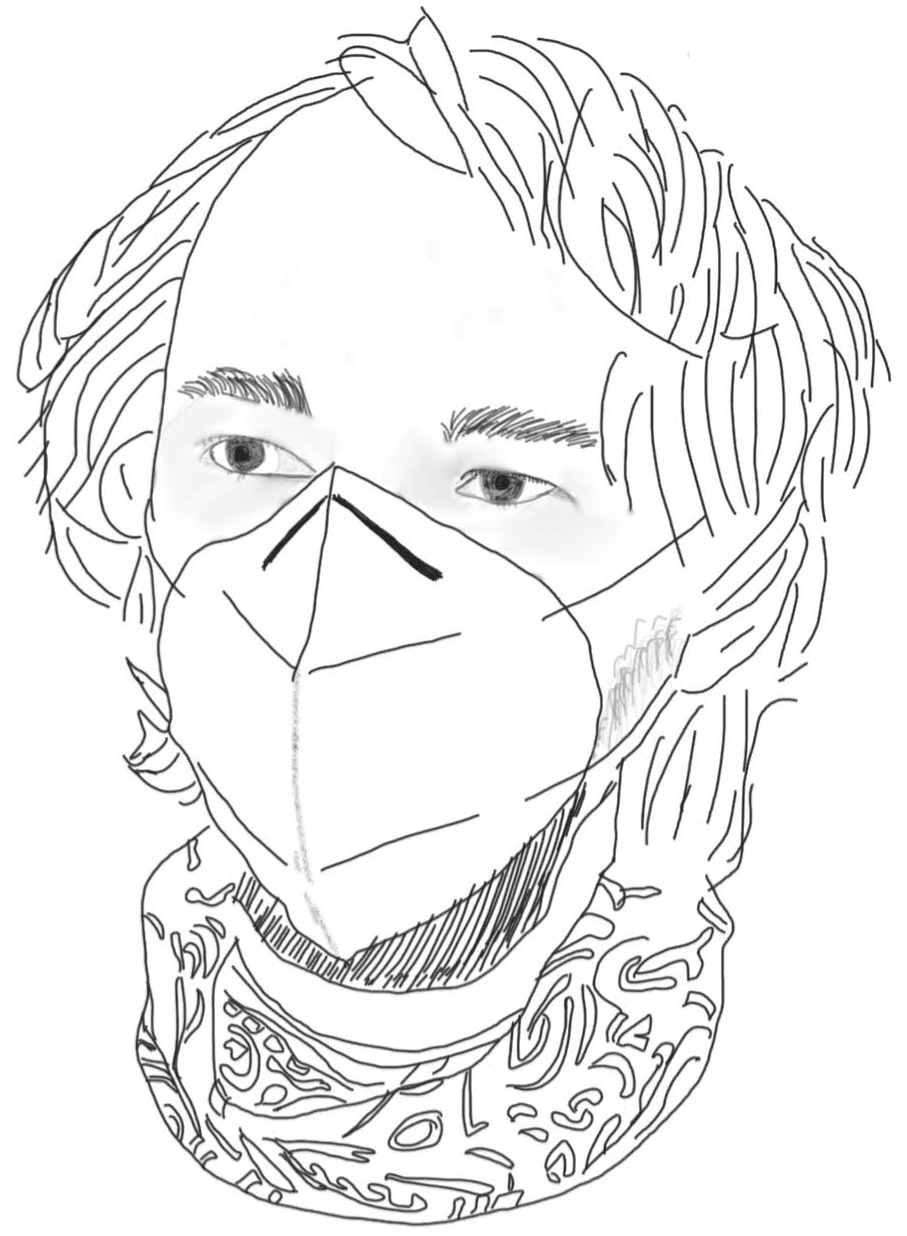
\includegraphics[height=2.5cm]{images/maskavatar-trimmed.jpg}
  \end{minipage}

  \vspace{5mm}
  \noindent
  
\includegraphics[height=1.8cm]{images/payments/qr-btc.pdf}\hspace{0.5cm}%
  
\includegraphics[height=1.8cm]{images/payments/qr-eth.pdf}\hspace{0.5cm}%
  \href{https://paypal.me/ralienpp}{
\includegraphics[height=1.8cm]{images/payments/qr-paypal.pdf}}%
  \hfill
  \href{https://creativecommons.org/licenses/by-sa/4.0/}{\includegraphics[height=0.4cm]{images/cc-by-sa-eps-converted-to.pdf}}
}

\end{document}
"
% ============================================================
%  main-dual.tex — Dual-language edition of
%                  "The Horse, the Dung, and the Car"
%
%  Renders two languages stacked per text block: the PRIMARY language
%  (\booklang) on top, the SECONDARY language (\booklangsecondary) below
%  it in \small\itshape. Body story pages are dual (\dualtr); the cover
%  and the parent-guide prose remain single-language (\tr, primary).
%
%  Languages are configurable. Defaults below: Romanian primary, English
%  secondary. Override from the command line, e.g.:
%    lualatex "\def\booklang{en}\def\booklangsecondary{ro}% !TeX program = lualatex
% !TeX options = -interaction=nonstopmode -halt-on-error "\def\booklang{ro}\def\booklangsecondary{en}\input{main-dual}"
% ============================================================
%  main-dual.tex — Dual-language edition of
%                  "The Horse, the Dung, and the Car"
%
%  Renders two languages stacked per text block: the PRIMARY language
%  (\booklang) on top, the SECONDARY language (\booklangsecondary) below
%  it in \small\itshape. Body story pages are dual (\dualtr); the cover
%  and the parent-guide prose remain single-language (\tr, primary).
%
%  Languages are configurable. Defaults below: Romanian primary, English
%  secondary. Override from the command line, e.g.:
%    lualatex "\def\booklang{en}\def\booklangsecondary{ro}\input{main-dual}"
%
%  Positions differ from main.tex: stacked blocks are taller, so several
%  bottom-anchored text blocks are moved up to keep both languages on the
%  page. main.tex is unchanged.
% ============================================================
\documentclass[17pt]{extarticle}

% --- Language configuration (override before \input to change) ---
\ifdefined\booklang\else\def\booklang{ro}\fi
\ifdefined\booklangsecondary\else\def\booklangsecondary{en}\fi

\def\bookfont{Antykwa Torunska}
%\def\bookfont{OpenDyslexic}
%\def\bookfontpath{fonts/opendyslexic/}
\usepackage[pagenumbers]{picturebook}
\usepackage{multicol}
\usepackage{hyperref}

% Secondary-language styling (optional overrides):
%   \renewcommand{\dualsecstyle}{\small\itshape}
%   \renewcommand{\dualsep}{\par\smallskip}

\begin{document}

% ============================================================
%  COVER (p.1) — modern city   [single language: primary]
% ============================================================
\pagenumbersoff
\singlepage{images/cover.jpeg}{1}{1}{12.8}{%
		\begin{center}
			{\Huge\bfseries \tr{title}}\\[0.5cm]
			{\large \tr{subtitle}}
		\end{center}
}
\block{1}{18}{12.8}{%
	\begin{center}
		{\small \tr{series}}
	\end{center}
}

% ============================================================
%  2x single pp.2–3 — horse tram era
% ============================================================
\pagenumberson
\singlepage{images/modern-city.jpeg}{3.5}{1}{10}{%
	\begin{halo}[color=white, opacity=0.3]
		\dualtr{p01_modern_city}
	\end{halo}
}


\singlepage{images/horse-tram.jpeg}{1}{1}{12.8}{%
	\begin{halo}[color=white, opacity=0.3]
		\dualtr{p02_horse_tram}
	\end{halo}
}

% ============================================================
%  p.4 — growing cities, growing horse population
% ============================================================
\singlepage{images/riders-carriages.jpeg}{1.5}{1}{8}{%
	\begin{halo}[color=white, opacity=0.5]
		\dualtr{p03_growing_cities}
	\end{halo}
}
% moved up (18 -> 15.5) to fit the stacked second language
\block{1}{15.5}{8}{%
	\begin{halo}[color=white, opacity=0.5]
		\dualtr{p03a_more_horses}
	\end{halo}
}

% ============================================================
%  p.5 — New York 1890 statistics
% ============================================================
% moved up (10 -> 8) to fit the stacked subtitle + second language
\singlepage{images/horse-human-pseudotessellation.png}{1}{8}{12.8}{%
	\begin{halo}[color=white, opacity=0.75]
		\dualtr{p04_ny_stats}

		\bigskip
		\dualtr{p04_ny_subtitle}
	\end{halo}
}

% ============================================================
%  SPREAD pp.6–7 — daily horse waste / smell
% ============================================================
\fullspread{images/horse-output.jpeg}%
{1}{1}{12}{% left page
	\begin{halo}[color=white, opacity=0.3]
		\dualtr{p05_manure_stats}

		\bigskip
		\dualtr{p05_subtitle}
	\end{halo}
}%
{2}{1}{10}{% right page — centered question
	\begin{halo}[color=white, opacity=0.3]
		\begin{center}
			{\Large\bfseries \dualtr{p06_smell}}
		\end{center}
	\end{halo}
}

% ============================================================
%  p.8 — alarming situation, people adapting
% ============================================================
\singlepage{images/street-manure.jpeg}{1}{0.5}{12.8}{%
	\begin{halo}[color=white, opacity=0.3]
		\dualtr{p07_alarming}
	\end{halo}
}

% ============================================================
%  p.9 — saved by technology (old car)
% ============================================================
% moved up (18 -> 14.5) — bottom-anchored block grows downward when stacked
\singlepage{images/benz-motorwagen.jpeg}{1}{15}{12.8}{%
	\begin{halo}[color=white, opacity=0.4]
		\dualtr{p08_saved_by_tech}
	\end{halo}
}

% ============================================================
%  SPREAD pp.10–11 — history repeats / growing cars
% ============================================================
\singlepage{images/car-human-pseudotessellation.jpeg}{2}{8}{10}{%
	\begin{halo}[color=yellow, opacity=0.5]
	\begin{center}
		{\Large\bfseries \dualtr{p09_history_repeats}}
	\end{center}
	\end{halo}
}


\singlepage{images/gridlock.jpg}{1}{1}{12}{%
	\begin{halo}[color=white, opacity=0.3]
		\dualtr{p10_cars_growing}
	\end{halo}
}

% ============================================================
%  p.12 — cars produce invisible exhaust
% ============================================================
\singlepage{images/shrouded-in-exhaust-gas-clear.jpeg}{1}{0.8}{12.8}{%
	\begin{halo}[color=white, opacity=0.3]
		\dualtr{p11_exhaust}
	\end{halo}
}

% ============================================================
%  p.13 — can be smelled / detected
% ============================================================
\singlepage{images/shrouded-in-exhaust-gas.jpeg}{1}{0.8}{12.8}{%
	\begin{halo}[color=white, opacity=0.3]
		\dualtr{p12_detect}
	\end{halo}
}

% ============================================================
%  SPREAD pp.14–15 — health effects / piles haven't disappeared
% ============================================================
\fullspread{images/coughing.jpeg}%
{1}{1}{12.8}{% left page
	\begin{halo}[color=white, opacity=0.3]
		\dualtr{p13_health}
	\end{halo}
}%
{2}{1}{10}{% right page — dramatic
	\begin{halo}[color=white, opacity=0.3]
		\begin{center}
			{\Large\bfseries \dualtr{p14_piles_back}}
		\end{center}
	\end{halo}
}

% ============================================================
%  p.16 — what can you do?
% ============================================================
\singlepage{images/what-can-i-do.jpeg}{2}{1}{10}{%
	\begin{halo}[color=white, opacity=0.8]
		\begin{center}
			{\Large\bfseries \dualtr{p15_what_can_you_do}}
		\end{center}
	\end{halo}
}

% ============================================================
%  p.17 — walk, bike, public transport
% ============================================================
\singlepage{images/walk.jpeg}{1}{1}{12.8}{%
		\begin{center}
			\dualtr{p16_walk}
		\end{center}
}


\singlepage{images/cyclists.jpeg}{1}{1}{12.8}{%
		\begin{center}
			\dualtr{p16_bike}
		\end{center}
}

\singlepage{images/train-valley.jpg}{1}{2}{12.8}{%
		\dualtr{p16_public_transport}
}

\singlepage{images/remote-call.jpeg}{1}{1}{12.8}{%
		\begin{center}
			\dualtr{p16_stay}
		\end{center}
}

% ============================================================
%  p.18 — plant a tree
% ============================================================
% moved up (17 -> 15) to fit the stacked second language
\singlepage{images/plant-tree.jpeg}{1}{17}{12.8}{%
		\dualtr{p17_plant_tree}
}

% ============================================================
%  p.19 — use your vote
% ============================================================
\singlepage{images/vote.jpeg}{7}{1}{7}{%
		\dualtr{p18_vote}
}

% ============================================================
%  p.20 — contribute to tech progress
% ============================================================
% moved up (19 -> 16.5) to fit the stacked second language
\singlepage{images/science.jpeg}{1}{16.5}{12.8}{%
	\begin{halo}[color=white, opacity=0.8]
		\dualtr{p19_tech_progress}
	\end{halo}
}


% ============================================================
%  p.21,22 — think about the ecosystem
% ============================================================

\fullspread{images/planet.jpeg}%
{2}{1}{10}{% left page
	\begin{center}
		{\Large\bfseries \dualtr{p20_ecosystem}}
	\end{center}
}%
{2}{1}{10}{% 
	
}

% ============================================================
%  PROSE SECTION — parent guide   [single language: primary]
% ============================================================
\pagenumberson
\pagenumberstyle{center}
\startprose
\section*{\tr{parent_guide_title}}
{\small \tr{parent_guide_body}}

% ============================================================
%  GLOSSARY — vocabulary with IPA and translations
% ============================================================
\ifdefined\bookglossaryoff\else
  \newpage
  \section*{\tr{glossary_title}}

  \printglossary{translations/glossary.csv}{\booklang}{\booklangsecondary}
\fi

% ============================================================
%  BACK COVER
%  Pad to a full saddle-stitch signature (multiple of 4 pages) so
%  the back cover lands on the physical back-cover surface.
% ============================================================
\padbooklet
\backcover{%
  {\noindent\textbf{\tr{other_books_title}}\par\smallskip}
  \begin{bookgrid}
	\book{images/covers/cat-tree.png}{Poetry for kids}
    \book{images/covers/cover-high5.png}{What is software engineering?}
	\book{images/covers/tree-cover.jpeg}{Never give up}
  \end{bookgrid}

  \vfill

  {\noindent\textbf{\tr{about_author_title}}\par\smallskip}
  \noindent
  \begin{minipage}[t]{0.75\textwidth}
    \footnotesize
    \tr{about_author_body}
  \end{minipage}%
  \hfill
  \begin{minipage}[t]{0.2\textwidth}
    \raggedleft
    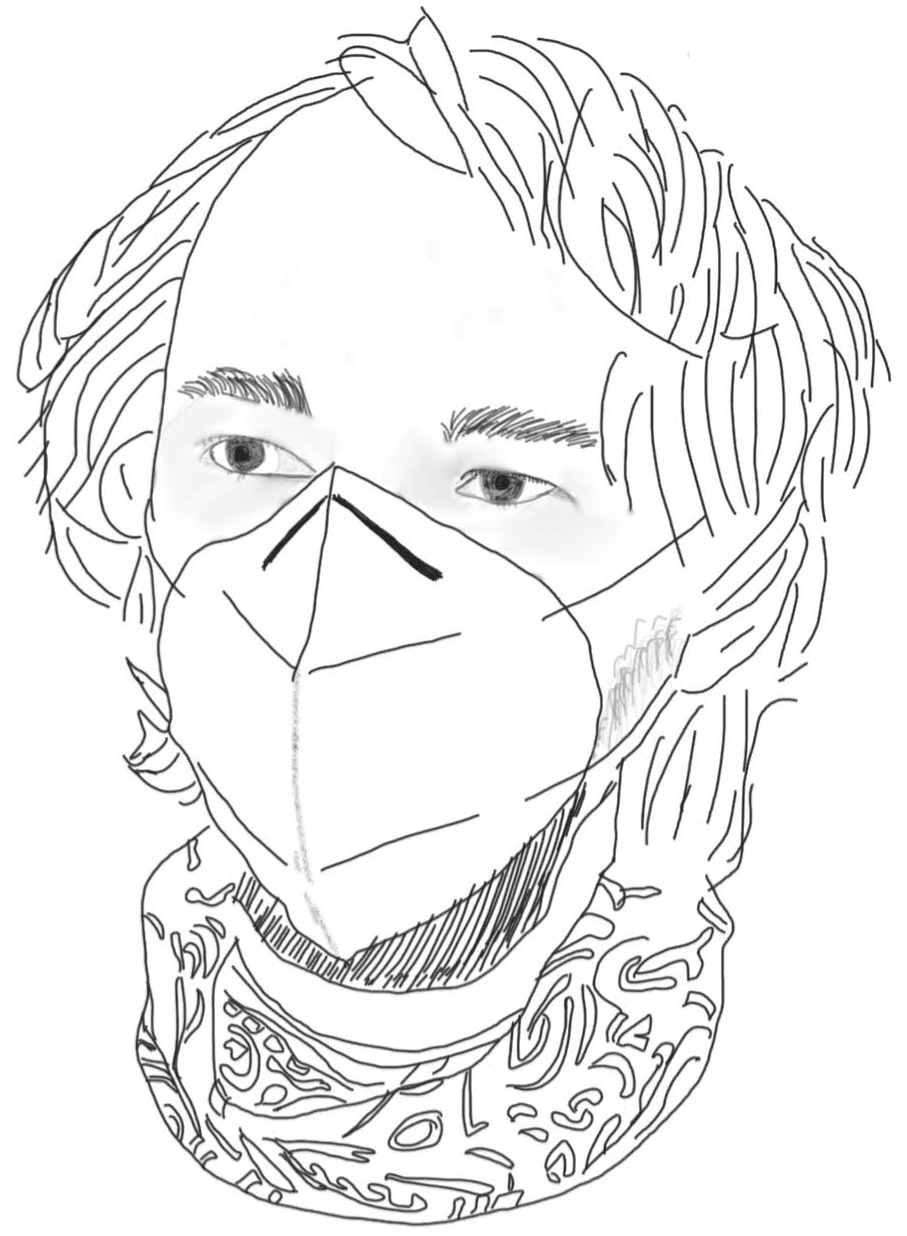
\includegraphics[height=2.5cm]{images/maskavatar-trimmed.jpg}
  \end{minipage}

  \vspace{5mm}
  \noindent
  
\includegraphics[height=1.8cm]{images/payments/qr-btc.pdf}\hspace{0.5cm}%
  
\includegraphics[height=1.8cm]{images/payments/qr-eth.pdf}\hspace{0.5cm}%
  \href{https://paypal.me/ralienpp}{
\includegraphics[height=1.8cm]{images/payments/qr-paypal.pdf}}%
  \hfill
  \href{https://creativecommons.org/licenses/by-sa/4.0/}{\includegraphics[height=0.4cm]{images/cc-by-sa-eps-converted-to.pdf}}
}

\end{document}
"
%
%  Positions differ from main.tex: stacked blocks are taller, so several
%  bottom-anchored text blocks are moved up to keep both languages on the
%  page. main.tex is unchanged.
% ============================================================
\documentclass[17pt]{extarticle}

% --- Language configuration (override before \input to change) ---
\ifdefined\booklang\else\def\booklang{ro}\fi
\ifdefined\booklangsecondary\else\def\booklangsecondary{en}\fi

\def\bookfont{Antykwa Torunska}
%\def\bookfont{OpenDyslexic}
%\def\bookfontpath{fonts/opendyslexic/}
\usepackage[pagenumbers]{picturebook}
\usepackage{multicol}
\usepackage{hyperref}

% Secondary-language styling (optional overrides):
%   \renewcommand{\dualsecstyle}{\small\itshape}
%   \renewcommand{\dualsep}{\par\smallskip}

\begin{document}

% ============================================================
%  COVER (p.1) — modern city   [single language: primary]
% ============================================================
\pagenumbersoff
\singlepage{images/cover.jpeg}{1}{1}{12.8}{%
		\begin{center}
			{\Huge\bfseries \tr{title}}\\[0.5cm]
			{\large \tr{subtitle}}
		\end{center}
}
\block{1}{18}{12.8}{%
	\begin{center}
		{\small \tr{series}}
	\end{center}
}

% ============================================================
%  2x single pp.2–3 — horse tram era
% ============================================================
\pagenumberson
\singlepage{images/modern-city.jpeg}{3.5}{1}{10}{%
	\begin{halo}[color=white, opacity=0.3]
		\dualtr{p01_modern_city}
	\end{halo}
}


\singlepage{images/horse-tram.jpeg}{1}{1}{12.8}{%
	\begin{halo}[color=white, opacity=0.3]
		\dualtr{p02_horse_tram}
	\end{halo}
}

% ============================================================
%  p.4 — growing cities, growing horse population
% ============================================================
\singlepage{images/riders-carriages.jpeg}{1.5}{1}{8}{%
	\begin{halo}[color=white, opacity=0.5]
		\dualtr{p03_growing_cities}
	\end{halo}
}
% moved up (18 -> 15.5) to fit the stacked second language
\block{1}{15.5}{8}{%
	\begin{halo}[color=white, opacity=0.5]
		\dualtr{p03a_more_horses}
	\end{halo}
}

% ============================================================
%  p.5 — New York 1890 statistics
% ============================================================
% moved up (10 -> 8) to fit the stacked subtitle + second language
\singlepage{images/horse-human-pseudotessellation.png}{1}{8}{12.8}{%
	\begin{halo}[color=white, opacity=0.75]
		\dualtr{p04_ny_stats}

		\bigskip
		\dualtr{p04_ny_subtitle}
	\end{halo}
}

% ============================================================
%  SPREAD pp.6–7 — daily horse waste / smell
% ============================================================
\fullspread{images/horse-output.jpeg}%
{1}{1}{12}{% left page
	\begin{halo}[color=white, opacity=0.3]
		\dualtr{p05_manure_stats}

		\bigskip
		\dualtr{p05_subtitle}
	\end{halo}
}%
{2}{1}{10}{% right page — centered question
	\begin{halo}[color=white, opacity=0.3]
		\begin{center}
			{\Large\bfseries \dualtr{p06_smell}}
		\end{center}
	\end{halo}
}

% ============================================================
%  p.8 — alarming situation, people adapting
% ============================================================
\singlepage{images/street-manure.jpeg}{1}{0.5}{12.8}{%
	\begin{halo}[color=white, opacity=0.3]
		\dualtr{p07_alarming}
	\end{halo}
}

% ============================================================
%  p.9 — saved by technology (old car)
% ============================================================
% moved up (18 -> 14.5) — bottom-anchored block grows downward when stacked
\singlepage{images/benz-motorwagen.jpeg}{1}{15}{12.8}{%
	\begin{halo}[color=white, opacity=0.4]
		\dualtr{p08_saved_by_tech}
	\end{halo}
}

% ============================================================
%  SPREAD pp.10–11 — history repeats / growing cars
% ============================================================
\singlepage{images/car-human-pseudotessellation.jpeg}{2}{8}{10}{%
	\begin{halo}[color=yellow, opacity=0.5]
	\begin{center}
		{\Large\bfseries \dualtr{p09_history_repeats}}
	\end{center}
	\end{halo}
}


\singlepage{images/gridlock.jpg}{1}{1}{12}{%
	\begin{halo}[color=white, opacity=0.3]
		\dualtr{p10_cars_growing}
	\end{halo}
}

% ============================================================
%  p.12 — cars produce invisible exhaust
% ============================================================
\singlepage{images/shrouded-in-exhaust-gas-clear.jpeg}{1}{0.8}{12.8}{%
	\begin{halo}[color=white, opacity=0.3]
		\dualtr{p11_exhaust}
	\end{halo}
}

% ============================================================
%  p.13 — can be smelled / detected
% ============================================================
\singlepage{images/shrouded-in-exhaust-gas.jpeg}{1}{0.8}{12.8}{%
	\begin{halo}[color=white, opacity=0.3]
		\dualtr{p12_detect}
	\end{halo}
}

% ============================================================
%  SPREAD pp.14–15 — health effects / piles haven't disappeared
% ============================================================
\fullspread{images/coughing.jpeg}%
{1}{1}{12.8}{% left page
	\begin{halo}[color=white, opacity=0.3]
		\dualtr{p13_health}
	\end{halo}
}%
{2}{1}{10}{% right page — dramatic
	\begin{halo}[color=white, opacity=0.3]
		\begin{center}
			{\Large\bfseries \dualtr{p14_piles_back}}
		\end{center}
	\end{halo}
}

% ============================================================
%  p.16 — what can you do?
% ============================================================
\singlepage{images/what-can-i-do.jpeg}{2}{1}{10}{%
	\begin{halo}[color=white, opacity=0.8]
		\begin{center}
			{\Large\bfseries \dualtr{p15_what_can_you_do}}
		\end{center}
	\end{halo}
}

% ============================================================
%  p.17 — walk, bike, public transport
% ============================================================
\singlepage{images/walk.jpeg}{1}{1}{12.8}{%
		\begin{center}
			\dualtr{p16_walk}
		\end{center}
}


\singlepage{images/cyclists.jpeg}{1}{1}{12.8}{%
		\begin{center}
			\dualtr{p16_bike}
		\end{center}
}

\singlepage{images/train-valley.jpg}{1}{2}{12.8}{%
		\dualtr{p16_public_transport}
}

\singlepage{images/remote-call.jpeg}{1}{1}{12.8}{%
		\begin{center}
			\dualtr{p16_stay}
		\end{center}
}

% ============================================================
%  p.18 — plant a tree
% ============================================================
% moved up (17 -> 15) to fit the stacked second language
\singlepage{images/plant-tree.jpeg}{1}{17}{12.8}{%
		\dualtr{p17_plant_tree}
}

% ============================================================
%  p.19 — use your vote
% ============================================================
\singlepage{images/vote.jpeg}{7}{1}{7}{%
		\dualtr{p18_vote}
}

% ============================================================
%  p.20 — contribute to tech progress
% ============================================================
% moved up (19 -> 16.5) to fit the stacked second language
\singlepage{images/science.jpeg}{1}{16.5}{12.8}{%
	\begin{halo}[color=white, opacity=0.8]
		\dualtr{p19_tech_progress}
	\end{halo}
}


% ============================================================
%  p.21,22 — think about the ecosystem
% ============================================================

\fullspread{images/planet.jpeg}%
{2}{1}{10}{% left page
	\begin{center}
		{\Large\bfseries \dualtr{p20_ecosystem}}
	\end{center}
}%
{2}{1}{10}{% 
	
}

% ============================================================
%  PROSE SECTION — parent guide   [single language: primary]
% ============================================================
\pagenumberson
\pagenumberstyle{center}
\startprose
\section*{\tr{parent_guide_title}}
{\small \tr{parent_guide_body}}

% ============================================================
%  GLOSSARY — vocabulary with IPA and translations
% ============================================================
\ifdefined\bookglossaryoff\else
  \newpage
  \section*{\tr{glossary_title}}

  \printglossary{translations/glossary.csv}{\booklang}{\booklangsecondary}
\fi

% ============================================================
%  BACK COVER
%  Pad to a full saddle-stitch signature (multiple of 4 pages) so
%  the back cover lands on the physical back-cover surface.
% ============================================================
\padbooklet
\backcover{%
  {\noindent\textbf{\tr{other_books_title}}\par\smallskip}
  \begin{bookgrid}
	\book{images/covers/cat-tree.png}{Poetry for kids}
    \book{images/covers/cover-high5.png}{What is software engineering?}
	\book{images/covers/tree-cover.jpeg}{Never give up}
  \end{bookgrid}

  \vfill

  {\noindent\textbf{\tr{about_author_title}}\par\smallskip}
  \noindent
  \begin{minipage}[t]{0.75\textwidth}
    \footnotesize
    \tr{about_author_body}
  \end{minipage}%
  \hfill
  \begin{minipage}[t]{0.2\textwidth}
    \raggedleft
    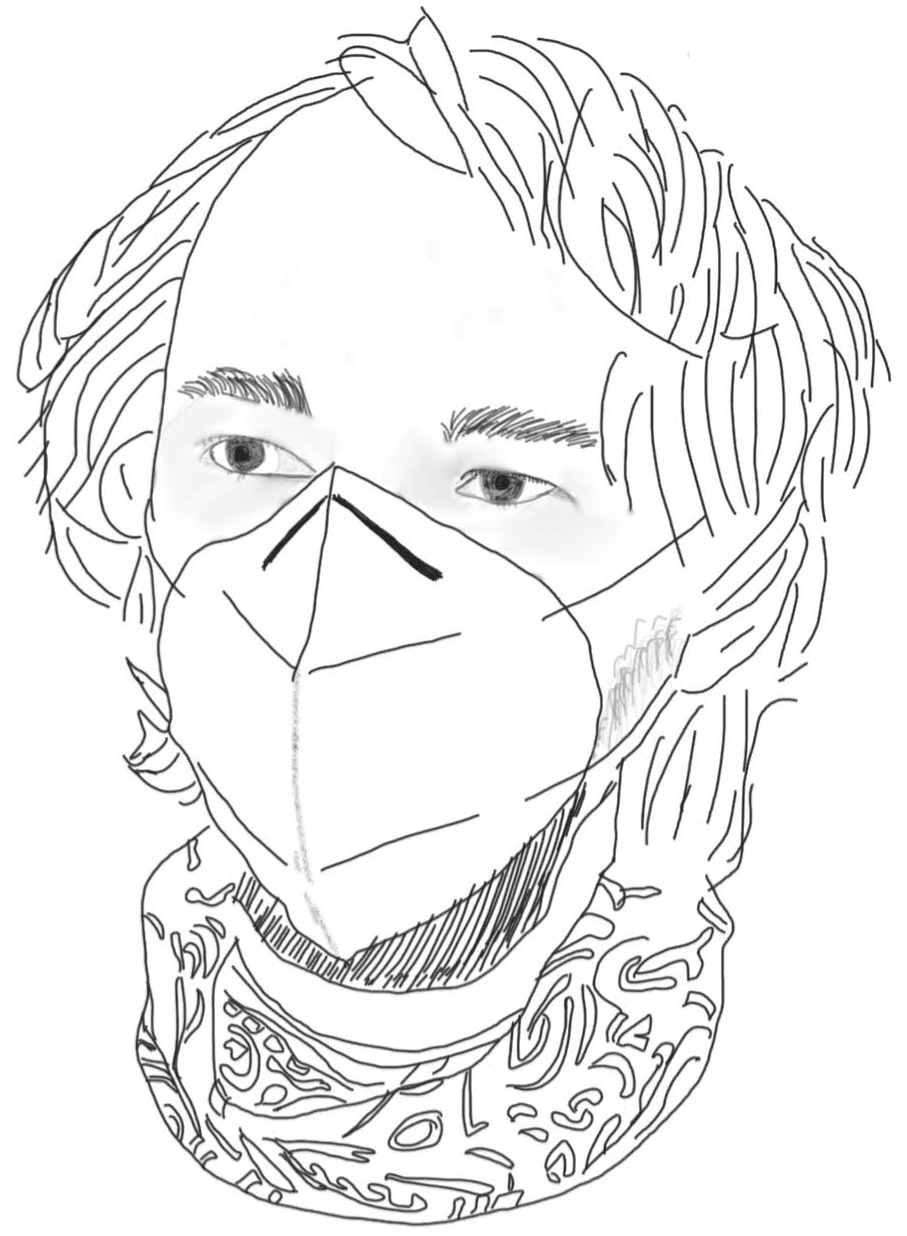
\includegraphics[height=2.5cm]{images/maskavatar-trimmed.jpg}
  \end{minipage}

  \vspace{5mm}
  \noindent
  
\includegraphics[height=1.8cm]{images/payments/qr-btc.pdf}\hspace{0.5cm}%
  
\includegraphics[height=1.8cm]{images/payments/qr-eth.pdf}\hspace{0.5cm}%
  \href{https://paypal.me/ralienpp}{
\includegraphics[height=1.8cm]{images/payments/qr-paypal.pdf}}%
  \hfill
  \href{https://creativecommons.org/licenses/by-sa/4.0/}{\includegraphics[height=0.4cm]{images/cc-by-sa-eps-converted-to.pdf}}
}

\end{document}
"
% ============================================================
%  main-dual.tex — Dual-language edition of
%                  "The Horse, the Dung, and the Car"
%
%  Renders two languages stacked per text block: the PRIMARY language
%  (\booklang) on top, the SECONDARY language (\booklangsecondary) below
%  it in \small\itshape. Body story pages are dual (\dualtr); the cover
%  and the parent-guide prose remain single-language (\tr, primary).
%
%  Languages are configurable. Defaults below: Romanian primary, English
%  secondary. Override from the command line, e.g.:
%    lualatex "\def\booklang{en}\def\booklangsecondary{ro}% !TeX program = lualatex
% !TeX options = -interaction=nonstopmode -halt-on-error "\def\booklang{ro}\def\booklangsecondary{en}% !TeX program = lualatex
% !TeX options = -interaction=nonstopmode -halt-on-error "\def\booklang{ro}\def\booklangsecondary{en}\input{main-dual}"
% ============================================================
%  main-dual.tex — Dual-language edition of
%                  "The Horse, the Dung, and the Car"
%
%  Renders two languages stacked per text block: the PRIMARY language
%  (\booklang) on top, the SECONDARY language (\booklangsecondary) below
%  it in \small\itshape. Body story pages are dual (\dualtr); the cover
%  and the parent-guide prose remain single-language (\tr, primary).
%
%  Languages are configurable. Defaults below: Romanian primary, English
%  secondary. Override from the command line, e.g.:
%    lualatex "\def\booklang{en}\def\booklangsecondary{ro}\input{main-dual}"
%
%  Positions differ from main.tex: stacked blocks are taller, so several
%  bottom-anchored text blocks are moved up to keep both languages on the
%  page. main.tex is unchanged.
% ============================================================
\documentclass[17pt]{extarticle}

% --- Language configuration (override before \input to change) ---
\ifdefined\booklang\else\def\booklang{ro}\fi
\ifdefined\booklangsecondary\else\def\booklangsecondary{en}\fi

\def\bookfont{Antykwa Torunska}
%\def\bookfont{OpenDyslexic}
%\def\bookfontpath{fonts/opendyslexic/}
\usepackage[pagenumbers]{picturebook}
\usepackage{multicol}
\usepackage{hyperref}

% Secondary-language styling (optional overrides):
%   \renewcommand{\dualsecstyle}{\small\itshape}
%   \renewcommand{\dualsep}{\par\smallskip}

\begin{document}

% ============================================================
%  COVER (p.1) — modern city   [single language: primary]
% ============================================================
\pagenumbersoff
\singlepage{images/cover.jpeg}{1}{1}{12.8}{%
		\begin{center}
			{\Huge\bfseries \tr{title}}\\[0.5cm]
			{\large \tr{subtitle}}
		\end{center}
}
\block{1}{18}{12.8}{%
	\begin{center}
		{\small \tr{series}}
	\end{center}
}

% ============================================================
%  2x single pp.2–3 — horse tram era
% ============================================================
\pagenumberson
\singlepage{images/modern-city.jpeg}{3.5}{1}{10}{%
	\begin{halo}[color=white, opacity=0.3]
		\dualtr{p01_modern_city}
	\end{halo}
}


\singlepage{images/horse-tram.jpeg}{1}{1}{12.8}{%
	\begin{halo}[color=white, opacity=0.3]
		\dualtr{p02_horse_tram}
	\end{halo}
}

% ============================================================
%  p.4 — growing cities, growing horse population
% ============================================================
\singlepage{images/riders-carriages.jpeg}{1.5}{1}{8}{%
	\begin{halo}[color=white, opacity=0.5]
		\dualtr{p03_growing_cities}
	\end{halo}
}
% moved up (18 -> 15.5) to fit the stacked second language
\block{1}{15.5}{8}{%
	\begin{halo}[color=white, opacity=0.5]
		\dualtr{p03a_more_horses}
	\end{halo}
}

% ============================================================
%  p.5 — New York 1890 statistics
% ============================================================
% moved up (10 -> 8) to fit the stacked subtitle + second language
\singlepage{images/horse-human-pseudotessellation.png}{1}{8}{12.8}{%
	\begin{halo}[color=white, opacity=0.75]
		\dualtr{p04_ny_stats}

		\bigskip
		\dualtr{p04_ny_subtitle}
	\end{halo}
}

% ============================================================
%  SPREAD pp.6–7 — daily horse waste / smell
% ============================================================
\fullspread{images/horse-output.jpeg}%
{1}{1}{12}{% left page
	\begin{halo}[color=white, opacity=0.3]
		\dualtr{p05_manure_stats}

		\bigskip
		\dualtr{p05_subtitle}
	\end{halo}
}%
{2}{1}{10}{% right page — centered question
	\begin{halo}[color=white, opacity=0.3]
		\begin{center}
			{\Large\bfseries \dualtr{p06_smell}}
		\end{center}
	\end{halo}
}

% ============================================================
%  p.8 — alarming situation, people adapting
% ============================================================
\singlepage{images/street-manure.jpeg}{1}{0.5}{12.8}{%
	\begin{halo}[color=white, opacity=0.3]
		\dualtr{p07_alarming}
	\end{halo}
}

% ============================================================
%  p.9 — saved by technology (old car)
% ============================================================
% moved up (18 -> 14.5) — bottom-anchored block grows downward when stacked
\singlepage{images/benz-motorwagen.jpeg}{1}{15}{12.8}{%
	\begin{halo}[color=white, opacity=0.4]
		\dualtr{p08_saved_by_tech}
	\end{halo}
}

% ============================================================
%  SPREAD pp.10–11 — history repeats / growing cars
% ============================================================
\singlepage{images/car-human-pseudotessellation.jpeg}{2}{8}{10}{%
	\begin{halo}[color=yellow, opacity=0.5]
	\begin{center}
		{\Large\bfseries \dualtr{p09_history_repeats}}
	\end{center}
	\end{halo}
}


\singlepage{images/gridlock.jpg}{1}{1}{12}{%
	\begin{halo}[color=white, opacity=0.3]
		\dualtr{p10_cars_growing}
	\end{halo}
}

% ============================================================
%  p.12 — cars produce invisible exhaust
% ============================================================
\singlepage{images/shrouded-in-exhaust-gas-clear.jpeg}{1}{0.8}{12.8}{%
	\begin{halo}[color=white, opacity=0.3]
		\dualtr{p11_exhaust}
	\end{halo}
}

% ============================================================
%  p.13 — can be smelled / detected
% ============================================================
\singlepage{images/shrouded-in-exhaust-gas.jpeg}{1}{0.8}{12.8}{%
	\begin{halo}[color=white, opacity=0.3]
		\dualtr{p12_detect}
	\end{halo}
}

% ============================================================
%  SPREAD pp.14–15 — health effects / piles haven't disappeared
% ============================================================
\fullspread{images/coughing.jpeg}%
{1}{1}{12.8}{% left page
	\begin{halo}[color=white, opacity=0.3]
		\dualtr{p13_health}
	\end{halo}
}%
{2}{1}{10}{% right page — dramatic
	\begin{halo}[color=white, opacity=0.3]
		\begin{center}
			{\Large\bfseries \dualtr{p14_piles_back}}
		\end{center}
	\end{halo}
}

% ============================================================
%  p.16 — what can you do?
% ============================================================
\singlepage{images/what-can-i-do.jpeg}{2}{1}{10}{%
	\begin{halo}[color=white, opacity=0.8]
		\begin{center}
			{\Large\bfseries \dualtr{p15_what_can_you_do}}
		\end{center}
	\end{halo}
}

% ============================================================
%  p.17 — walk, bike, public transport
% ============================================================
\singlepage{images/walk.jpeg}{1}{1}{12.8}{%
		\begin{center}
			\dualtr{p16_walk}
		\end{center}
}


\singlepage{images/cyclists.jpeg}{1}{1}{12.8}{%
		\begin{center}
			\dualtr{p16_bike}
		\end{center}
}

\singlepage{images/train-valley.jpg}{1}{2}{12.8}{%
		\dualtr{p16_public_transport}
}

\singlepage{images/remote-call.jpeg}{1}{1}{12.8}{%
		\begin{center}
			\dualtr{p16_stay}
		\end{center}
}

% ============================================================
%  p.18 — plant a tree
% ============================================================
% moved up (17 -> 15) to fit the stacked second language
\singlepage{images/plant-tree.jpeg}{1}{17}{12.8}{%
		\dualtr{p17_plant_tree}
}

% ============================================================
%  p.19 — use your vote
% ============================================================
\singlepage{images/vote.jpeg}{7}{1}{7}{%
		\dualtr{p18_vote}
}

% ============================================================
%  p.20 — contribute to tech progress
% ============================================================
% moved up (19 -> 16.5) to fit the stacked second language
\singlepage{images/science.jpeg}{1}{16.5}{12.8}{%
	\begin{halo}[color=white, opacity=0.8]
		\dualtr{p19_tech_progress}
	\end{halo}
}


% ============================================================
%  p.21,22 — think about the ecosystem
% ============================================================

\fullspread{images/planet.jpeg}%
{2}{1}{10}{% left page
	\begin{center}
		{\Large\bfseries \dualtr{p20_ecosystem}}
	\end{center}
}%
{2}{1}{10}{% 
	
}

% ============================================================
%  PROSE SECTION — parent guide   [single language: primary]
% ============================================================
\pagenumberson
\pagenumberstyle{center}
\startprose
\section*{\tr{parent_guide_title}}
{\small \tr{parent_guide_body}}

% ============================================================
%  GLOSSARY — vocabulary with IPA and translations
% ============================================================
\ifdefined\bookglossaryoff\else
  \newpage
  \section*{\tr{glossary_title}}

  \printglossary{translations/glossary.csv}{\booklang}{\booklangsecondary}
\fi

% ============================================================
%  BACK COVER
%  Pad to a full saddle-stitch signature (multiple of 4 pages) so
%  the back cover lands on the physical back-cover surface.
% ============================================================
\padbooklet
\backcover{%
  {\noindent\textbf{\tr{other_books_title}}\par\smallskip}
  \begin{bookgrid}
	\book{images/covers/cat-tree.png}{Poetry for kids}
    \book{images/covers/cover-high5.png}{What is software engineering?}
	\book{images/covers/tree-cover.jpeg}{Never give up}
  \end{bookgrid}

  \vfill

  {\noindent\textbf{\tr{about_author_title}}\par\smallskip}
  \noindent
  \begin{minipage}[t]{0.75\textwidth}
    \footnotesize
    \tr{about_author_body}
  \end{minipage}%
  \hfill
  \begin{minipage}[t]{0.2\textwidth}
    \raggedleft
    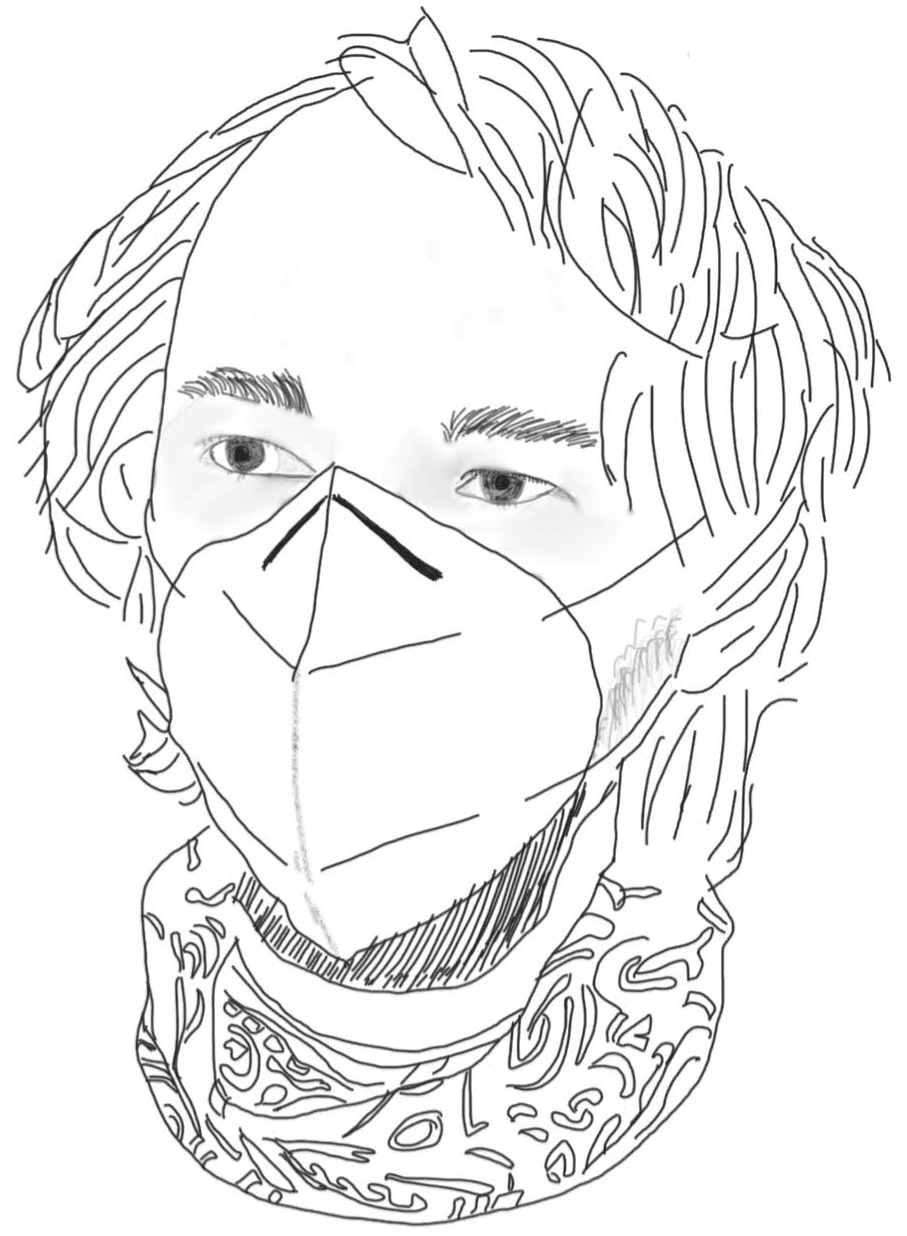
\includegraphics[height=2.5cm]{images/maskavatar-trimmed.jpg}
  \end{minipage}

  \vspace{5mm}
  \noindent
  
\includegraphics[height=1.8cm]{images/payments/qr-btc.pdf}\hspace{0.5cm}%
  
\includegraphics[height=1.8cm]{images/payments/qr-eth.pdf}\hspace{0.5cm}%
  \href{https://paypal.me/ralienpp}{
\includegraphics[height=1.8cm]{images/payments/qr-paypal.pdf}}%
  \hfill
  \href{https://creativecommons.org/licenses/by-sa/4.0/}{\includegraphics[height=0.4cm]{images/cc-by-sa-eps-converted-to.pdf}}
}

\end{document}
"
% ============================================================
%  main-dual.tex — Dual-language edition of
%                  "The Horse, the Dung, and the Car"
%
%  Renders two languages stacked per text block: the PRIMARY language
%  (\booklang) on top, the SECONDARY language (\booklangsecondary) below
%  it in \small\itshape. Body story pages are dual (\dualtr); the cover
%  and the parent-guide prose remain single-language (\tr, primary).
%
%  Languages are configurable. Defaults below: Romanian primary, English
%  secondary. Override from the command line, e.g.:
%    lualatex "\def\booklang{en}\def\booklangsecondary{ro}% !TeX program = lualatex
% !TeX options = -interaction=nonstopmode -halt-on-error "\def\booklang{ro}\def\booklangsecondary{en}\input{main-dual}"
% ============================================================
%  main-dual.tex — Dual-language edition of
%                  "The Horse, the Dung, and the Car"
%
%  Renders two languages stacked per text block: the PRIMARY language
%  (\booklang) on top, the SECONDARY language (\booklangsecondary) below
%  it in \small\itshape. Body story pages are dual (\dualtr); the cover
%  and the parent-guide prose remain single-language (\tr, primary).
%
%  Languages are configurable. Defaults below: Romanian primary, English
%  secondary. Override from the command line, e.g.:
%    lualatex "\def\booklang{en}\def\booklangsecondary{ro}\input{main-dual}"
%
%  Positions differ from main.tex: stacked blocks are taller, so several
%  bottom-anchored text blocks are moved up to keep both languages on the
%  page. main.tex is unchanged.
% ============================================================
\documentclass[17pt]{extarticle}

% --- Language configuration (override before \input to change) ---
\ifdefined\booklang\else\def\booklang{ro}\fi
\ifdefined\booklangsecondary\else\def\booklangsecondary{en}\fi

\def\bookfont{Antykwa Torunska}
%\def\bookfont{OpenDyslexic}
%\def\bookfontpath{fonts/opendyslexic/}
\usepackage[pagenumbers]{picturebook}
\usepackage{multicol}
\usepackage{hyperref}

% Secondary-language styling (optional overrides):
%   \renewcommand{\dualsecstyle}{\small\itshape}
%   \renewcommand{\dualsep}{\par\smallskip}

\begin{document}

% ============================================================
%  COVER (p.1) — modern city   [single language: primary]
% ============================================================
\pagenumbersoff
\singlepage{images/cover.jpeg}{1}{1}{12.8}{%
		\begin{center}
			{\Huge\bfseries \tr{title}}\\[0.5cm]
			{\large \tr{subtitle}}
		\end{center}
}
\block{1}{18}{12.8}{%
	\begin{center}
		{\small \tr{series}}
	\end{center}
}

% ============================================================
%  2x single pp.2–3 — horse tram era
% ============================================================
\pagenumberson
\singlepage{images/modern-city.jpeg}{3.5}{1}{10}{%
	\begin{halo}[color=white, opacity=0.3]
		\dualtr{p01_modern_city}
	\end{halo}
}


\singlepage{images/horse-tram.jpeg}{1}{1}{12.8}{%
	\begin{halo}[color=white, opacity=0.3]
		\dualtr{p02_horse_tram}
	\end{halo}
}

% ============================================================
%  p.4 — growing cities, growing horse population
% ============================================================
\singlepage{images/riders-carriages.jpeg}{1.5}{1}{8}{%
	\begin{halo}[color=white, opacity=0.5]
		\dualtr{p03_growing_cities}
	\end{halo}
}
% moved up (18 -> 15.5) to fit the stacked second language
\block{1}{15.5}{8}{%
	\begin{halo}[color=white, opacity=0.5]
		\dualtr{p03a_more_horses}
	\end{halo}
}

% ============================================================
%  p.5 — New York 1890 statistics
% ============================================================
% moved up (10 -> 8) to fit the stacked subtitle + second language
\singlepage{images/horse-human-pseudotessellation.png}{1}{8}{12.8}{%
	\begin{halo}[color=white, opacity=0.75]
		\dualtr{p04_ny_stats}

		\bigskip
		\dualtr{p04_ny_subtitle}
	\end{halo}
}

% ============================================================
%  SPREAD pp.6–7 — daily horse waste / smell
% ============================================================
\fullspread{images/horse-output.jpeg}%
{1}{1}{12}{% left page
	\begin{halo}[color=white, opacity=0.3]
		\dualtr{p05_manure_stats}

		\bigskip
		\dualtr{p05_subtitle}
	\end{halo}
}%
{2}{1}{10}{% right page — centered question
	\begin{halo}[color=white, opacity=0.3]
		\begin{center}
			{\Large\bfseries \dualtr{p06_smell}}
		\end{center}
	\end{halo}
}

% ============================================================
%  p.8 — alarming situation, people adapting
% ============================================================
\singlepage{images/street-manure.jpeg}{1}{0.5}{12.8}{%
	\begin{halo}[color=white, opacity=0.3]
		\dualtr{p07_alarming}
	\end{halo}
}

% ============================================================
%  p.9 — saved by technology (old car)
% ============================================================
% moved up (18 -> 14.5) — bottom-anchored block grows downward when stacked
\singlepage{images/benz-motorwagen.jpeg}{1}{15}{12.8}{%
	\begin{halo}[color=white, opacity=0.4]
		\dualtr{p08_saved_by_tech}
	\end{halo}
}

% ============================================================
%  SPREAD pp.10–11 — history repeats / growing cars
% ============================================================
\singlepage{images/car-human-pseudotessellation.jpeg}{2}{8}{10}{%
	\begin{halo}[color=yellow, opacity=0.5]
	\begin{center}
		{\Large\bfseries \dualtr{p09_history_repeats}}
	\end{center}
	\end{halo}
}


\singlepage{images/gridlock.jpg}{1}{1}{12}{%
	\begin{halo}[color=white, opacity=0.3]
		\dualtr{p10_cars_growing}
	\end{halo}
}

% ============================================================
%  p.12 — cars produce invisible exhaust
% ============================================================
\singlepage{images/shrouded-in-exhaust-gas-clear.jpeg}{1}{0.8}{12.8}{%
	\begin{halo}[color=white, opacity=0.3]
		\dualtr{p11_exhaust}
	\end{halo}
}

% ============================================================
%  p.13 — can be smelled / detected
% ============================================================
\singlepage{images/shrouded-in-exhaust-gas.jpeg}{1}{0.8}{12.8}{%
	\begin{halo}[color=white, opacity=0.3]
		\dualtr{p12_detect}
	\end{halo}
}

% ============================================================
%  SPREAD pp.14–15 — health effects / piles haven't disappeared
% ============================================================
\fullspread{images/coughing.jpeg}%
{1}{1}{12.8}{% left page
	\begin{halo}[color=white, opacity=0.3]
		\dualtr{p13_health}
	\end{halo}
}%
{2}{1}{10}{% right page — dramatic
	\begin{halo}[color=white, opacity=0.3]
		\begin{center}
			{\Large\bfseries \dualtr{p14_piles_back}}
		\end{center}
	\end{halo}
}

% ============================================================
%  p.16 — what can you do?
% ============================================================
\singlepage{images/what-can-i-do.jpeg}{2}{1}{10}{%
	\begin{halo}[color=white, opacity=0.8]
		\begin{center}
			{\Large\bfseries \dualtr{p15_what_can_you_do}}
		\end{center}
	\end{halo}
}

% ============================================================
%  p.17 — walk, bike, public transport
% ============================================================
\singlepage{images/walk.jpeg}{1}{1}{12.8}{%
		\begin{center}
			\dualtr{p16_walk}
		\end{center}
}


\singlepage{images/cyclists.jpeg}{1}{1}{12.8}{%
		\begin{center}
			\dualtr{p16_bike}
		\end{center}
}

\singlepage{images/train-valley.jpg}{1}{2}{12.8}{%
		\dualtr{p16_public_transport}
}

\singlepage{images/remote-call.jpeg}{1}{1}{12.8}{%
		\begin{center}
			\dualtr{p16_stay}
		\end{center}
}

% ============================================================
%  p.18 — plant a tree
% ============================================================
% moved up (17 -> 15) to fit the stacked second language
\singlepage{images/plant-tree.jpeg}{1}{17}{12.8}{%
		\dualtr{p17_plant_tree}
}

% ============================================================
%  p.19 — use your vote
% ============================================================
\singlepage{images/vote.jpeg}{7}{1}{7}{%
		\dualtr{p18_vote}
}

% ============================================================
%  p.20 — contribute to tech progress
% ============================================================
% moved up (19 -> 16.5) to fit the stacked second language
\singlepage{images/science.jpeg}{1}{16.5}{12.8}{%
	\begin{halo}[color=white, opacity=0.8]
		\dualtr{p19_tech_progress}
	\end{halo}
}


% ============================================================
%  p.21,22 — think about the ecosystem
% ============================================================

\fullspread{images/planet.jpeg}%
{2}{1}{10}{% left page
	\begin{center}
		{\Large\bfseries \dualtr{p20_ecosystem}}
	\end{center}
}%
{2}{1}{10}{% 
	
}

% ============================================================
%  PROSE SECTION — parent guide   [single language: primary]
% ============================================================
\pagenumberson
\pagenumberstyle{center}
\startprose
\section*{\tr{parent_guide_title}}
{\small \tr{parent_guide_body}}

% ============================================================
%  GLOSSARY — vocabulary with IPA and translations
% ============================================================
\ifdefined\bookglossaryoff\else
  \newpage
  \section*{\tr{glossary_title}}

  \printglossary{translations/glossary.csv}{\booklang}{\booklangsecondary}
\fi

% ============================================================
%  BACK COVER
%  Pad to a full saddle-stitch signature (multiple of 4 pages) so
%  the back cover lands on the physical back-cover surface.
% ============================================================
\padbooklet
\backcover{%
  {\noindent\textbf{\tr{other_books_title}}\par\smallskip}
  \begin{bookgrid}
	\book{images/covers/cat-tree.png}{Poetry for kids}
    \book{images/covers/cover-high5.png}{What is software engineering?}
	\book{images/covers/tree-cover.jpeg}{Never give up}
  \end{bookgrid}

  \vfill

  {\noindent\textbf{\tr{about_author_title}}\par\smallskip}
  \noindent
  \begin{minipage}[t]{0.75\textwidth}
    \footnotesize
    \tr{about_author_body}
  \end{minipage}%
  \hfill
  \begin{minipage}[t]{0.2\textwidth}
    \raggedleft
    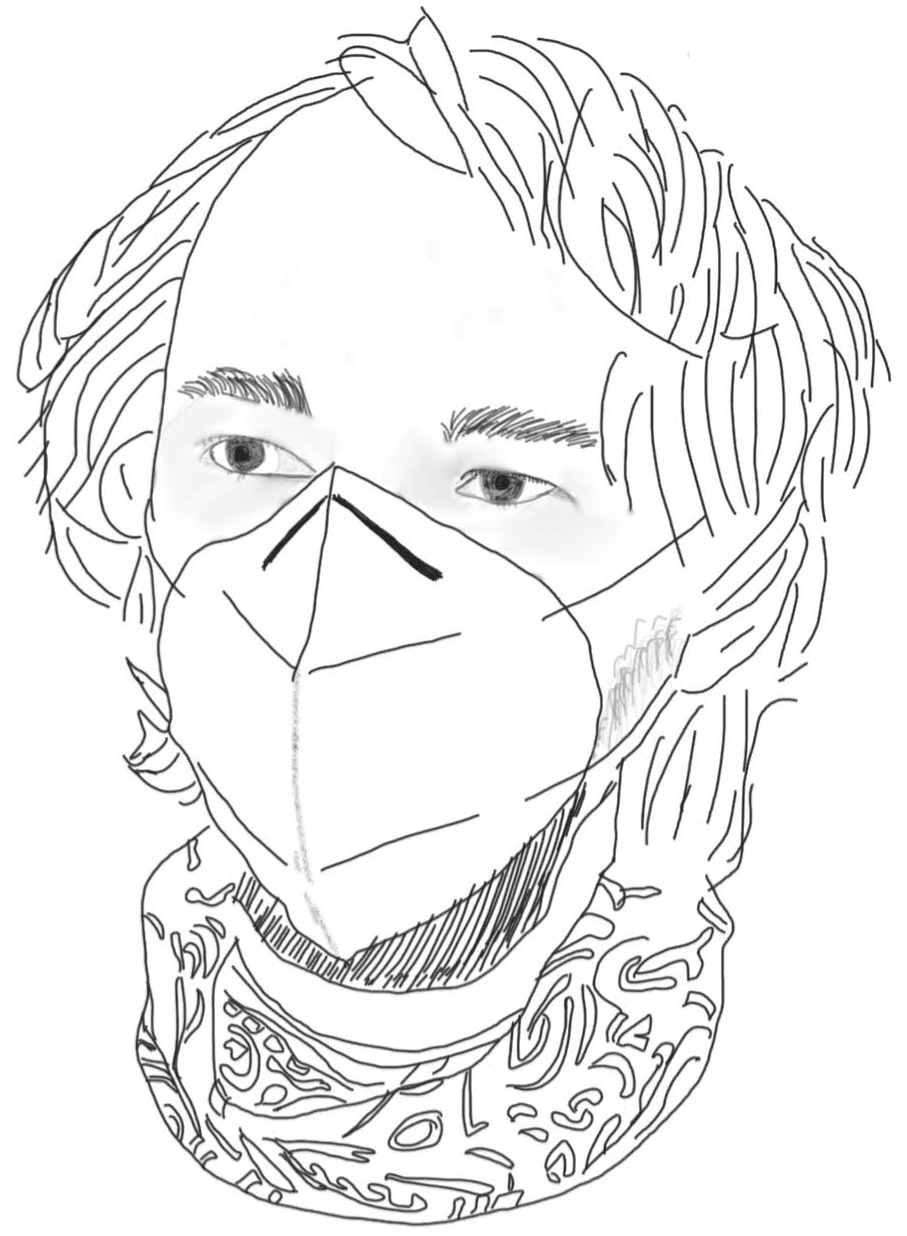
\includegraphics[height=2.5cm]{images/maskavatar-trimmed.jpg}
  \end{minipage}

  \vspace{5mm}
  \noindent
  
\includegraphics[height=1.8cm]{images/payments/qr-btc.pdf}\hspace{0.5cm}%
  
\includegraphics[height=1.8cm]{images/payments/qr-eth.pdf}\hspace{0.5cm}%
  \href{https://paypal.me/ralienpp}{
\includegraphics[height=1.8cm]{images/payments/qr-paypal.pdf}}%
  \hfill
  \href{https://creativecommons.org/licenses/by-sa/4.0/}{\includegraphics[height=0.4cm]{images/cc-by-sa-eps-converted-to.pdf}}
}

\end{document}
"
%
%  Positions differ from main.tex: stacked blocks are taller, so several
%  bottom-anchored text blocks are moved up to keep both languages on the
%  page. main.tex is unchanged.
% ============================================================
\documentclass[17pt]{extarticle}

% --- Language configuration (override before \input to change) ---
\ifdefined\booklang\else\def\booklang{ro}\fi
\ifdefined\booklangsecondary\else\def\booklangsecondary{en}\fi

\def\bookfont{Antykwa Torunska}
%\def\bookfont{OpenDyslexic}
%\def\bookfontpath{fonts/opendyslexic/}
\usepackage[pagenumbers]{picturebook}
\usepackage{multicol}
\usepackage{hyperref}

% Secondary-language styling (optional overrides):
%   \renewcommand{\dualsecstyle}{\small\itshape}
%   \renewcommand{\dualsep}{\par\smallskip}

\begin{document}

% ============================================================
%  COVER (p.1) — modern city   [single language: primary]
% ============================================================
\pagenumbersoff
\singlepage{images/cover.jpeg}{1}{1}{12.8}{%
		\begin{center}
			{\Huge\bfseries \tr{title}}\\[0.5cm]
			{\large \tr{subtitle}}
		\end{center}
}
\block{1}{18}{12.8}{%
	\begin{center}
		{\small \tr{series}}
	\end{center}
}

% ============================================================
%  2x single pp.2–3 — horse tram era
% ============================================================
\pagenumberson
\singlepage{images/modern-city.jpeg}{3.5}{1}{10}{%
	\begin{halo}[color=white, opacity=0.3]
		\dualtr{p01_modern_city}
	\end{halo}
}


\singlepage{images/horse-tram.jpeg}{1}{1}{12.8}{%
	\begin{halo}[color=white, opacity=0.3]
		\dualtr{p02_horse_tram}
	\end{halo}
}

% ============================================================
%  p.4 — growing cities, growing horse population
% ============================================================
\singlepage{images/riders-carriages.jpeg}{1.5}{1}{8}{%
	\begin{halo}[color=white, opacity=0.5]
		\dualtr{p03_growing_cities}
	\end{halo}
}
% moved up (18 -> 15.5) to fit the stacked second language
\block{1}{15.5}{8}{%
	\begin{halo}[color=white, opacity=0.5]
		\dualtr{p03a_more_horses}
	\end{halo}
}

% ============================================================
%  p.5 — New York 1890 statistics
% ============================================================
% moved up (10 -> 8) to fit the stacked subtitle + second language
\singlepage{images/horse-human-pseudotessellation.png}{1}{8}{12.8}{%
	\begin{halo}[color=white, opacity=0.75]
		\dualtr{p04_ny_stats}

		\bigskip
		\dualtr{p04_ny_subtitle}
	\end{halo}
}

% ============================================================
%  SPREAD pp.6–7 — daily horse waste / smell
% ============================================================
\fullspread{images/horse-output.jpeg}%
{1}{1}{12}{% left page
	\begin{halo}[color=white, opacity=0.3]
		\dualtr{p05_manure_stats}

		\bigskip
		\dualtr{p05_subtitle}
	\end{halo}
}%
{2}{1}{10}{% right page — centered question
	\begin{halo}[color=white, opacity=0.3]
		\begin{center}
			{\Large\bfseries \dualtr{p06_smell}}
		\end{center}
	\end{halo}
}

% ============================================================
%  p.8 — alarming situation, people adapting
% ============================================================
\singlepage{images/street-manure.jpeg}{1}{0.5}{12.8}{%
	\begin{halo}[color=white, opacity=0.3]
		\dualtr{p07_alarming}
	\end{halo}
}

% ============================================================
%  p.9 — saved by technology (old car)
% ============================================================
% moved up (18 -> 14.5) — bottom-anchored block grows downward when stacked
\singlepage{images/benz-motorwagen.jpeg}{1}{15}{12.8}{%
	\begin{halo}[color=white, opacity=0.4]
		\dualtr{p08_saved_by_tech}
	\end{halo}
}

% ============================================================
%  SPREAD pp.10–11 — history repeats / growing cars
% ============================================================
\singlepage{images/car-human-pseudotessellation.jpeg}{2}{8}{10}{%
	\begin{halo}[color=yellow, opacity=0.5]
	\begin{center}
		{\Large\bfseries \dualtr{p09_history_repeats}}
	\end{center}
	\end{halo}
}


\singlepage{images/gridlock.jpg}{1}{1}{12}{%
	\begin{halo}[color=white, opacity=0.3]
		\dualtr{p10_cars_growing}
	\end{halo}
}

% ============================================================
%  p.12 — cars produce invisible exhaust
% ============================================================
\singlepage{images/shrouded-in-exhaust-gas-clear.jpeg}{1}{0.8}{12.8}{%
	\begin{halo}[color=white, opacity=0.3]
		\dualtr{p11_exhaust}
	\end{halo}
}

% ============================================================
%  p.13 — can be smelled / detected
% ============================================================
\singlepage{images/shrouded-in-exhaust-gas.jpeg}{1}{0.8}{12.8}{%
	\begin{halo}[color=white, opacity=0.3]
		\dualtr{p12_detect}
	\end{halo}
}

% ============================================================
%  SPREAD pp.14–15 — health effects / piles haven't disappeared
% ============================================================
\fullspread{images/coughing.jpeg}%
{1}{1}{12.8}{% left page
	\begin{halo}[color=white, opacity=0.3]
		\dualtr{p13_health}
	\end{halo}
}%
{2}{1}{10}{% right page — dramatic
	\begin{halo}[color=white, opacity=0.3]
		\begin{center}
			{\Large\bfseries \dualtr{p14_piles_back}}
		\end{center}
	\end{halo}
}

% ============================================================
%  p.16 — what can you do?
% ============================================================
\singlepage{images/what-can-i-do.jpeg}{2}{1}{10}{%
	\begin{halo}[color=white, opacity=0.8]
		\begin{center}
			{\Large\bfseries \dualtr{p15_what_can_you_do}}
		\end{center}
	\end{halo}
}

% ============================================================
%  p.17 — walk, bike, public transport
% ============================================================
\singlepage{images/walk.jpeg}{1}{1}{12.8}{%
		\begin{center}
			\dualtr{p16_walk}
		\end{center}
}


\singlepage{images/cyclists.jpeg}{1}{1}{12.8}{%
		\begin{center}
			\dualtr{p16_bike}
		\end{center}
}

\singlepage{images/train-valley.jpg}{1}{2}{12.8}{%
		\dualtr{p16_public_transport}
}

\singlepage{images/remote-call.jpeg}{1}{1}{12.8}{%
		\begin{center}
			\dualtr{p16_stay}
		\end{center}
}

% ============================================================
%  p.18 — plant a tree
% ============================================================
% moved up (17 -> 15) to fit the stacked second language
\singlepage{images/plant-tree.jpeg}{1}{17}{12.8}{%
		\dualtr{p17_plant_tree}
}

% ============================================================
%  p.19 — use your vote
% ============================================================
\singlepage{images/vote.jpeg}{7}{1}{7}{%
		\dualtr{p18_vote}
}

% ============================================================
%  p.20 — contribute to tech progress
% ============================================================
% moved up (19 -> 16.5) to fit the stacked second language
\singlepage{images/science.jpeg}{1}{16.5}{12.8}{%
	\begin{halo}[color=white, opacity=0.8]
		\dualtr{p19_tech_progress}
	\end{halo}
}


% ============================================================
%  p.21,22 — think about the ecosystem
% ============================================================

\fullspread{images/planet.jpeg}%
{2}{1}{10}{% left page
	\begin{center}
		{\Large\bfseries \dualtr{p20_ecosystem}}
	\end{center}
}%
{2}{1}{10}{% 
	
}

% ============================================================
%  PROSE SECTION — parent guide   [single language: primary]
% ============================================================
\pagenumberson
\pagenumberstyle{center}
\startprose
\section*{\tr{parent_guide_title}}
{\small \tr{parent_guide_body}}

% ============================================================
%  GLOSSARY — vocabulary with IPA and translations
% ============================================================
\ifdefined\bookglossaryoff\else
  \newpage
  \section*{\tr{glossary_title}}

  \printglossary{translations/glossary.csv}{\booklang}{\booklangsecondary}
\fi

% ============================================================
%  BACK COVER
%  Pad to a full saddle-stitch signature (multiple of 4 pages) so
%  the back cover lands on the physical back-cover surface.
% ============================================================
\padbooklet
\backcover{%
  {\noindent\textbf{\tr{other_books_title}}\par\smallskip}
  \begin{bookgrid}
	\book{images/covers/cat-tree.png}{Poetry for kids}
    \book{images/covers/cover-high5.png}{What is software engineering?}
	\book{images/covers/tree-cover.jpeg}{Never give up}
  \end{bookgrid}

  \vfill

  {\noindent\textbf{\tr{about_author_title}}\par\smallskip}
  \noindent
  \begin{minipage}[t]{0.75\textwidth}
    \footnotesize
    \tr{about_author_body}
  \end{minipage}%
  \hfill
  \begin{minipage}[t]{0.2\textwidth}
    \raggedleft
    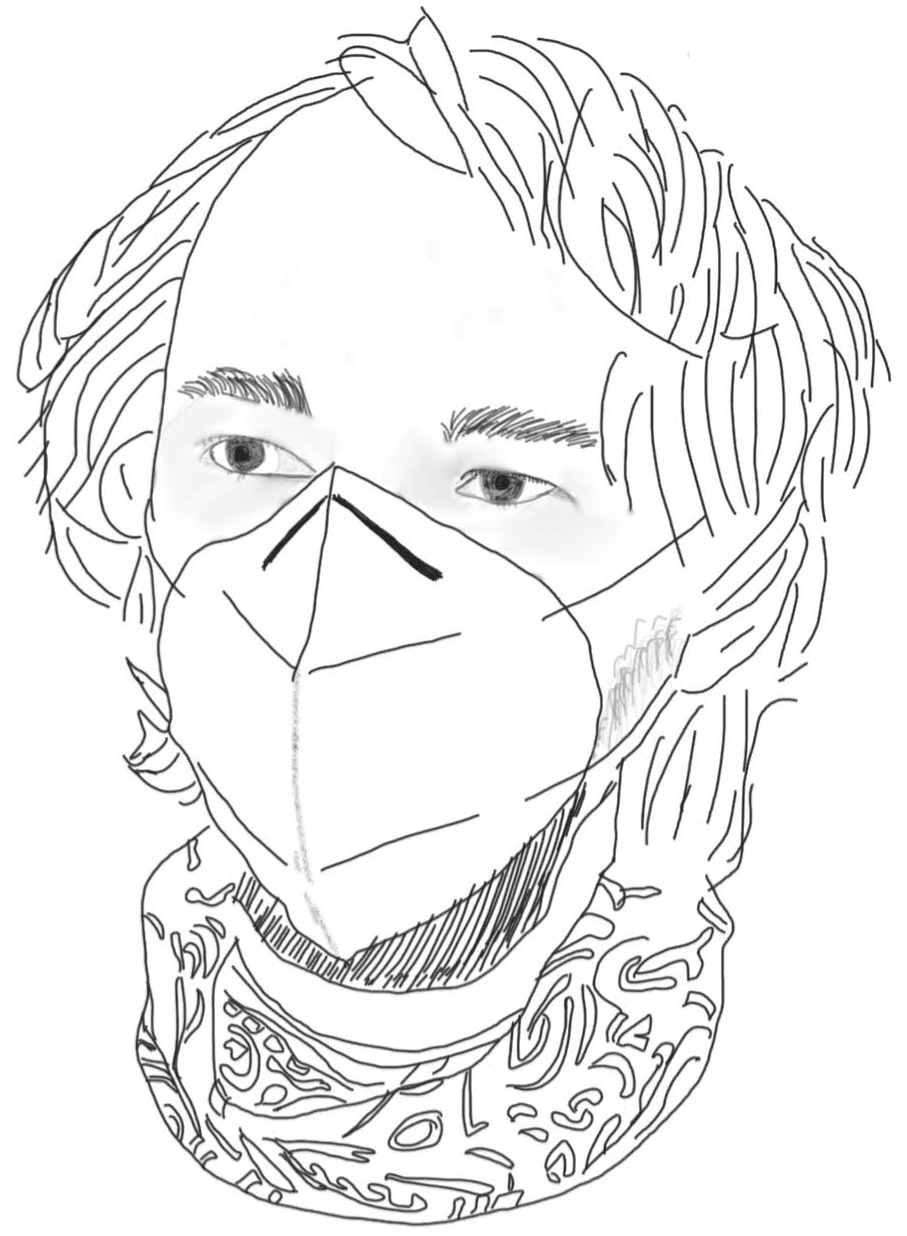
\includegraphics[height=2.5cm]{images/maskavatar-trimmed.jpg}
  \end{minipage}

  \vspace{5mm}
  \noindent
  
\includegraphics[height=1.8cm]{images/payments/qr-btc.pdf}\hspace{0.5cm}%
  
\includegraphics[height=1.8cm]{images/payments/qr-eth.pdf}\hspace{0.5cm}%
  \href{https://paypal.me/ralienpp}{
\includegraphics[height=1.8cm]{images/payments/qr-paypal.pdf}}%
  \hfill
  \href{https://creativecommons.org/licenses/by-sa/4.0/}{\includegraphics[height=0.4cm]{images/cc-by-sa-eps-converted-to.pdf}}
}

\end{document}
"
%
%  Positions differ from main.tex: stacked blocks are taller, so several
%  bottom-anchored text blocks are moved up to keep both languages on the
%  page. main.tex is unchanged.
% ============================================================
\documentclass[17pt]{extarticle}

% --- Language configuration (override before \input to change) ---
\ifdefined\booklang\else\def\booklang{ro}\fi
\ifdefined\booklangsecondary\else\def\booklangsecondary{en}\fi

\def\bookfont{Antykwa Torunska}
%\def\bookfont{OpenDyslexic}
%\def\bookfontpath{fonts/opendyslexic/}
\usepackage[pagenumbers]{picturebook}
\usepackage{multicol}
\usepackage{hyperref}

% Secondary-language styling (optional overrides):
%   \renewcommand{\dualsecstyle}{\small\itshape}
%   \renewcommand{\dualsep}{\par\smallskip}

\begin{document}

% ============================================================
%  COVER (p.1) — modern city   [single language: primary]
% ============================================================
\pagenumbersoff
\singlepage{images/cover.jpeg}{1}{1}{12.8}{%
		\begin{center}
			{\Huge\bfseries \tr{title}}\\[0.5cm]
			{\large \tr{subtitle}}
		\end{center}
}
\block{1}{18}{12.8}{%
	\begin{center}
		{\small \tr{series}}
	\end{center}
}

% ============================================================
%  2x single pp.2–3 — horse tram era
% ============================================================
\pagenumberson
\singlepage{images/modern-city.jpeg}{3.5}{1}{10}{%
	\begin{halo}[color=white, opacity=0.3]
		\dualtr{p01_modern_city}
	\end{halo}
}


\singlepage{images/horse-tram.jpeg}{1}{1}{12.8}{%
	\begin{halo}[color=white, opacity=0.3]
		\dualtr{p02_horse_tram}
	\end{halo}
}

% ============================================================
%  p.4 — growing cities, growing horse population
% ============================================================
\singlepage{images/riders-carriages.jpeg}{1.5}{1}{8}{%
	\begin{halo}[color=white, opacity=0.5]
		\dualtr{p03_growing_cities}
	\end{halo}
}
% moved up (18 -> 15.5) to fit the stacked second language
\block{1}{15.5}{8}{%
	\begin{halo}[color=white, opacity=0.5]
		\dualtr{p03a_more_horses}
	\end{halo}
}

% ============================================================
%  p.5 — New York 1890 statistics
% ============================================================
% moved up (10 -> 8) to fit the stacked subtitle + second language
\singlepage{images/horse-human-pseudotessellation.png}{1}{8}{12.8}{%
	\begin{halo}[color=white, opacity=0.75]
		\dualtr{p04_ny_stats}

		\bigskip
		\dualtr{p04_ny_subtitle}
	\end{halo}
}

% ============================================================
%  SPREAD pp.6–7 — daily horse waste / smell
% ============================================================
\fullspread{images/horse-output.jpeg}%
{1}{1}{12}{% left page
	\begin{halo}[color=white, opacity=0.3]
		\dualtr{p05_manure_stats}

		\bigskip
		\dualtr{p05_subtitle}
	\end{halo}
}%
{2}{1}{10}{% right page — centered question
	\begin{halo}[color=white, opacity=0.3]
		\begin{center}
			{\Large\bfseries \dualtr{p06_smell}}
		\end{center}
	\end{halo}
}

% ============================================================
%  p.8 — alarming situation, people adapting
% ============================================================
\singlepage{images/street-manure.jpeg}{1}{0.5}{12.8}{%
	\begin{halo}[color=white, opacity=0.3]
		\dualtr{p07_alarming}
	\end{halo}
}

% ============================================================
%  p.9 — saved by technology (old car)
% ============================================================
% moved up (18 -> 14.5) — bottom-anchored block grows downward when stacked
\singlepage{images/benz-motorwagen.jpeg}{1}{15}{12.8}{%
	\begin{halo}[color=white, opacity=0.4]
		\dualtr{p08_saved_by_tech}
	\end{halo}
}

% ============================================================
%  SPREAD pp.10–11 — history repeats / growing cars
% ============================================================
\singlepage{images/car-human-pseudotessellation.jpeg}{2}{8}{10}{%
	\begin{halo}[color=yellow, opacity=0.5]
	\begin{center}
		{\Large\bfseries \dualtr{p09_history_repeats}}
	\end{center}
	\end{halo}
}


\singlepage{images/gridlock.jpg}{1}{1}{12}{%
	\begin{halo}[color=white, opacity=0.3]
		\dualtr{p10_cars_growing}
	\end{halo}
}

% ============================================================
%  p.12 — cars produce invisible exhaust
% ============================================================
\singlepage{images/shrouded-in-exhaust-gas-clear.jpeg}{1}{0.8}{12.8}{%
	\begin{halo}[color=white, opacity=0.3]
		\dualtr{p11_exhaust}
	\end{halo}
}

% ============================================================
%  p.13 — can be smelled / detected
% ============================================================
\singlepage{images/shrouded-in-exhaust-gas.jpeg}{1}{0.8}{12.8}{%
	\begin{halo}[color=white, opacity=0.3]
		\dualtr{p12_detect}
	\end{halo}
}

% ============================================================
%  SPREAD pp.14–15 — health effects / piles haven't disappeared
% ============================================================
\fullspread{images/coughing.jpeg}%
{1}{1}{12.8}{% left page
	\begin{halo}[color=white, opacity=0.3]
		\dualtr{p13_health}
	\end{halo}
}%
{2}{1}{10}{% right page — dramatic
	\begin{halo}[color=white, opacity=0.3]
		\begin{center}
			{\Large\bfseries \dualtr{p14_piles_back}}
		\end{center}
	\end{halo}
}

% ============================================================
%  p.16 — what can you do?
% ============================================================
\singlepage{images/what-can-i-do.jpeg}{2}{1}{10}{%
	\begin{halo}[color=white, opacity=0.8]
		\begin{center}
			{\Large\bfseries \dualtr{p15_what_can_you_do}}
		\end{center}
	\end{halo}
}

% ============================================================
%  p.17 — walk, bike, public transport
% ============================================================
\singlepage{images/walk.jpeg}{1}{1}{12.8}{%
		\begin{center}
			\dualtr{p16_walk}
		\end{center}
}


\singlepage{images/cyclists.jpeg}{1}{1}{12.8}{%
		\begin{center}
			\dualtr{p16_bike}
		\end{center}
}

\singlepage{images/train-valley.jpg}{1}{2}{12.8}{%
		\dualtr{p16_public_transport}
}

\singlepage{images/remote-call.jpeg}{1}{1}{12.8}{%
		\begin{center}
			\dualtr{p16_stay}
		\end{center}
}

% ============================================================
%  p.18 — plant a tree
% ============================================================
% moved up (17 -> 15) to fit the stacked second language
\singlepage{images/plant-tree.jpeg}{1}{17}{12.8}{%
		\dualtr{p17_plant_tree}
}

% ============================================================
%  p.19 — use your vote
% ============================================================
\singlepage{images/vote.jpeg}{7}{1}{7}{%
		\dualtr{p18_vote}
}

% ============================================================
%  p.20 — contribute to tech progress
% ============================================================
% moved up (19 -> 16.5) to fit the stacked second language
\singlepage{images/science.jpeg}{1}{16.5}{12.8}{%
	\begin{halo}[color=white, opacity=0.8]
		\dualtr{p19_tech_progress}
	\end{halo}
}


% ============================================================
%  p.21,22 — think about the ecosystem
% ============================================================

\fullspread{images/planet.jpeg}%
{2}{1}{10}{% left page
	\begin{center}
		{\Large\bfseries \dualtr{p20_ecosystem}}
	\end{center}
}%
{2}{1}{10}{% 
	
}

% ============================================================
%  PROSE SECTION — parent guide   [single language: primary]
% ============================================================
\pagenumberson
\pagenumberstyle{center}
\startprose
\section*{\tr{parent_guide_title}}
{\small \tr{parent_guide_body}}

% ============================================================
%  GLOSSARY — vocabulary with IPA and translations
% ============================================================
\ifdefined\bookglossaryoff\else
  \newpage
  \section*{\tr{glossary_title}}

  \printglossary{translations/glossary.csv}{\booklang}{\booklangsecondary}
\fi

% ============================================================
%  BACK COVER
%  Pad to a full saddle-stitch signature (multiple of 4 pages) so
%  the back cover lands on the physical back-cover surface.
% ============================================================
\padbooklet
\backcover{%
  {\noindent\textbf{\tr{other_books_title}}\par\smallskip}
  \begin{bookgrid}
	\book{images/covers/cat-tree.png}{Poetry for kids}
    \book{images/covers/cover-high5.png}{What is software engineering?}
	\book{images/covers/tree-cover.jpeg}{Never give up}
  \end{bookgrid}

  \vfill

  {\noindent\textbf{\tr{about_author_title}}\par\smallskip}
  \noindent
  \begin{minipage}[t]{0.75\textwidth}
    \footnotesize
    \tr{about_author_body}
  \end{minipage}%
  \hfill
  \begin{minipage}[t]{0.2\textwidth}
    \raggedleft
    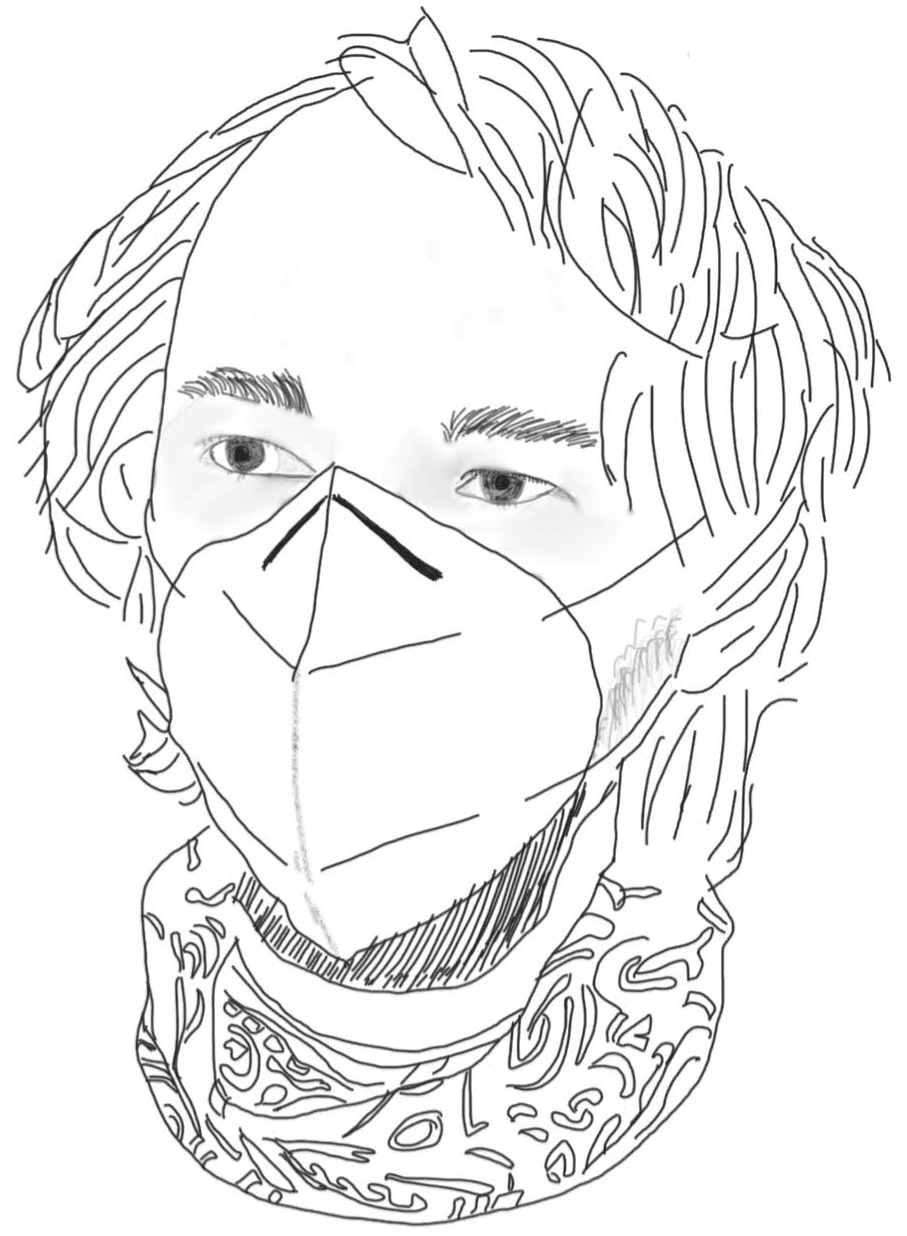
\includegraphics[height=2.5cm]{images/maskavatar-trimmed.jpg}
  \end{minipage}

  \vspace{5mm}
  \noindent
  
\includegraphics[height=1.8cm]{images/payments/qr-btc.pdf}\hspace{0.5cm}%
  
\includegraphics[height=1.8cm]{images/payments/qr-eth.pdf}\hspace{0.5cm}%
  \href{https://paypal.me/ralienpp}{
\includegraphics[height=1.8cm]{images/payments/qr-paypal.pdf}}%
  \hfill
  \href{https://creativecommons.org/licenses/by-sa/4.0/}{\includegraphics[height=0.4cm]{images/cc-by-sa-eps-converted-to.pdf}}
}

\end{document}
"
% ============================================================
%  main-dual.tex — Dual-language edition of
%                  "The Horse, the Dung, and the Car"
%
%  Renders two languages stacked per text block: the PRIMARY language
%  (\booklang) on top, the SECONDARY language (\booklangsecondary) below
%  it in \small\itshape. Body story pages are dual (\dualtr); the cover
%  and the parent-guide prose remain single-language (\tr, primary).
%
%  Languages are configurable. Defaults below: Romanian primary, English
%  secondary. Override from the command line, e.g.:
%    lualatex "\def\booklang{en}\def\booklangsecondary{ro}% !TeX program = lualatex
% !TeX options = -interaction=nonstopmode -halt-on-error "\def\booklang{ro}\def\booklangsecondary{en}% !TeX program = lualatex
% !TeX options = -interaction=nonstopmode -halt-on-error "\def\booklang{ro}\def\booklangsecondary{en}% !TeX program = lualatex
% !TeX options = -interaction=nonstopmode -halt-on-error "\def\booklang{ro}\def\booklangsecondary{en}\input{main-dual}"
% ============================================================
%  main-dual.tex — Dual-language edition of
%                  "The Horse, the Dung, and the Car"
%
%  Renders two languages stacked per text block: the PRIMARY language
%  (\booklang) on top, the SECONDARY language (\booklangsecondary) below
%  it in \small\itshape. Body story pages are dual (\dualtr); the cover
%  and the parent-guide prose remain single-language (\tr, primary).
%
%  Languages are configurable. Defaults below: Romanian primary, English
%  secondary. Override from the command line, e.g.:
%    lualatex "\def\booklang{en}\def\booklangsecondary{ro}\input{main-dual}"
%
%  Positions differ from main.tex: stacked blocks are taller, so several
%  bottom-anchored text blocks are moved up to keep both languages on the
%  page. main.tex is unchanged.
% ============================================================
\documentclass[17pt]{extarticle}

% --- Language configuration (override before \input to change) ---
\ifdefined\booklang\else\def\booklang{ro}\fi
\ifdefined\booklangsecondary\else\def\booklangsecondary{en}\fi

\def\bookfont{Antykwa Torunska}
%\def\bookfont{OpenDyslexic}
%\def\bookfontpath{fonts/opendyslexic/}
\usepackage[pagenumbers]{picturebook}
\usepackage{multicol}
\usepackage{hyperref}

% Secondary-language styling (optional overrides):
%   \renewcommand{\dualsecstyle}{\small\itshape}
%   \renewcommand{\dualsep}{\par\smallskip}

\begin{document}

% ============================================================
%  COVER (p.1) — modern city   [single language: primary]
% ============================================================
\pagenumbersoff
\singlepage{images/cover.jpeg}{1}{1}{12.8}{%
		\begin{center}
			{\Huge\bfseries \tr{title}}\\[0.5cm]
			{\large \tr{subtitle}}
		\end{center}
}
\block{1}{18}{12.8}{%
	\begin{center}
		{\small \tr{series}}
	\end{center}
}

% ============================================================
%  2x single pp.2–3 — horse tram era
% ============================================================
\pagenumberson
\singlepage{images/modern-city.jpeg}{3.5}{1}{10}{%
	\begin{halo}[color=white, opacity=0.3]
		\dualtr{p01_modern_city}
	\end{halo}
}


\singlepage{images/horse-tram.jpeg}{1}{1}{12.8}{%
	\begin{halo}[color=white, opacity=0.3]
		\dualtr{p02_horse_tram}
	\end{halo}
}

% ============================================================
%  p.4 — growing cities, growing horse population
% ============================================================
\singlepage{images/riders-carriages.jpeg}{1.5}{1}{8}{%
	\begin{halo}[color=white, opacity=0.5]
		\dualtr{p03_growing_cities}
	\end{halo}
}
% moved up (18 -> 15.5) to fit the stacked second language
\block{1}{15.5}{8}{%
	\begin{halo}[color=white, opacity=0.5]
		\dualtr{p03a_more_horses}
	\end{halo}
}

% ============================================================
%  p.5 — New York 1890 statistics
% ============================================================
% moved up (10 -> 8) to fit the stacked subtitle + second language
\singlepage{images/horse-human-pseudotessellation.png}{1}{8}{12.8}{%
	\begin{halo}[color=white, opacity=0.75]
		\dualtr{p04_ny_stats}

		\bigskip
		\dualtr{p04_ny_subtitle}
	\end{halo}
}

% ============================================================
%  SPREAD pp.6–7 — daily horse waste / smell
% ============================================================
\fullspread{images/horse-output.jpeg}%
{1}{1}{12}{% left page
	\begin{halo}[color=white, opacity=0.3]
		\dualtr{p05_manure_stats}

		\bigskip
		\dualtr{p05_subtitle}
	\end{halo}
}%
{2}{1}{10}{% right page — centered question
	\begin{halo}[color=white, opacity=0.3]
		\begin{center}
			{\Large\bfseries \dualtr{p06_smell}}
		\end{center}
	\end{halo}
}

% ============================================================
%  p.8 — alarming situation, people adapting
% ============================================================
\singlepage{images/street-manure.jpeg}{1}{0.5}{12.8}{%
	\begin{halo}[color=white, opacity=0.3]
		\dualtr{p07_alarming}
	\end{halo}
}

% ============================================================
%  p.9 — saved by technology (old car)
% ============================================================
% moved up (18 -> 14.5) — bottom-anchored block grows downward when stacked
\singlepage{images/benz-motorwagen.jpeg}{1}{15}{12.8}{%
	\begin{halo}[color=white, opacity=0.4]
		\dualtr{p08_saved_by_tech}
	\end{halo}
}

% ============================================================
%  SPREAD pp.10–11 — history repeats / growing cars
% ============================================================
\singlepage{images/car-human-pseudotessellation.jpeg}{2}{8}{10}{%
	\begin{halo}[color=yellow, opacity=0.5]
	\begin{center}
		{\Large\bfseries \dualtr{p09_history_repeats}}
	\end{center}
	\end{halo}
}


\singlepage{images/gridlock.jpg}{1}{1}{12}{%
	\begin{halo}[color=white, opacity=0.3]
		\dualtr{p10_cars_growing}
	\end{halo}
}

% ============================================================
%  p.12 — cars produce invisible exhaust
% ============================================================
\singlepage{images/shrouded-in-exhaust-gas-clear.jpeg}{1}{0.8}{12.8}{%
	\begin{halo}[color=white, opacity=0.3]
		\dualtr{p11_exhaust}
	\end{halo}
}

% ============================================================
%  p.13 — can be smelled / detected
% ============================================================
\singlepage{images/shrouded-in-exhaust-gas.jpeg}{1}{0.8}{12.8}{%
	\begin{halo}[color=white, opacity=0.3]
		\dualtr{p12_detect}
	\end{halo}
}

% ============================================================
%  SPREAD pp.14–15 — health effects / piles haven't disappeared
% ============================================================
\fullspread{images/coughing.jpeg}%
{1}{1}{12.8}{% left page
	\begin{halo}[color=white, opacity=0.3]
		\dualtr{p13_health}
	\end{halo}
}%
{2}{1}{10}{% right page — dramatic
	\begin{halo}[color=white, opacity=0.3]
		\begin{center}
			{\Large\bfseries \dualtr{p14_piles_back}}
		\end{center}
	\end{halo}
}

% ============================================================
%  p.16 — what can you do?
% ============================================================
\singlepage{images/what-can-i-do.jpeg}{2}{1}{10}{%
	\begin{halo}[color=white, opacity=0.8]
		\begin{center}
			{\Large\bfseries \dualtr{p15_what_can_you_do}}
		\end{center}
	\end{halo}
}

% ============================================================
%  p.17 — walk, bike, public transport
% ============================================================
\singlepage{images/walk.jpeg}{1}{1}{12.8}{%
		\begin{center}
			\dualtr{p16_walk}
		\end{center}
}


\singlepage{images/cyclists.jpeg}{1}{1}{12.8}{%
		\begin{center}
			\dualtr{p16_bike}
		\end{center}
}

\singlepage{images/train-valley.jpg}{1}{2}{12.8}{%
		\dualtr{p16_public_transport}
}

\singlepage{images/remote-call.jpeg}{1}{1}{12.8}{%
		\begin{center}
			\dualtr{p16_stay}
		\end{center}
}

% ============================================================
%  p.18 — plant a tree
% ============================================================
% moved up (17 -> 15) to fit the stacked second language
\singlepage{images/plant-tree.jpeg}{1}{17}{12.8}{%
		\dualtr{p17_plant_tree}
}

% ============================================================
%  p.19 — use your vote
% ============================================================
\singlepage{images/vote.jpeg}{7}{1}{7}{%
		\dualtr{p18_vote}
}

% ============================================================
%  p.20 — contribute to tech progress
% ============================================================
% moved up (19 -> 16.5) to fit the stacked second language
\singlepage{images/science.jpeg}{1}{16.5}{12.8}{%
	\begin{halo}[color=white, opacity=0.8]
		\dualtr{p19_tech_progress}
	\end{halo}
}


% ============================================================
%  p.21,22 — think about the ecosystem
% ============================================================

\fullspread{images/planet.jpeg}%
{2}{1}{10}{% left page
	\begin{center}
		{\Large\bfseries \dualtr{p20_ecosystem}}
	\end{center}
}%
{2}{1}{10}{% 
	
}

% ============================================================
%  PROSE SECTION — parent guide   [single language: primary]
% ============================================================
\pagenumberson
\pagenumberstyle{center}
\startprose
\section*{\tr{parent_guide_title}}
{\small \tr{parent_guide_body}}

% ============================================================
%  GLOSSARY — vocabulary with IPA and translations
% ============================================================
\ifdefined\bookglossaryoff\else
  \newpage
  \section*{\tr{glossary_title}}

  \printglossary{translations/glossary.csv}{\booklang}{\booklangsecondary}
\fi

% ============================================================
%  BACK COVER
%  Pad to a full saddle-stitch signature (multiple of 4 pages) so
%  the back cover lands on the physical back-cover surface.
% ============================================================
\padbooklet
\backcover{%
  {\noindent\textbf{\tr{other_books_title}}\par\smallskip}
  \begin{bookgrid}
	\book{images/covers/cat-tree.png}{Poetry for kids}
    \book{images/covers/cover-high5.png}{What is software engineering?}
	\book{images/covers/tree-cover.jpeg}{Never give up}
  \end{bookgrid}

  \vfill

  {\noindent\textbf{\tr{about_author_title}}\par\smallskip}
  \noindent
  \begin{minipage}[t]{0.75\textwidth}
    \footnotesize
    \tr{about_author_body}
  \end{minipage}%
  \hfill
  \begin{minipage}[t]{0.2\textwidth}
    \raggedleft
    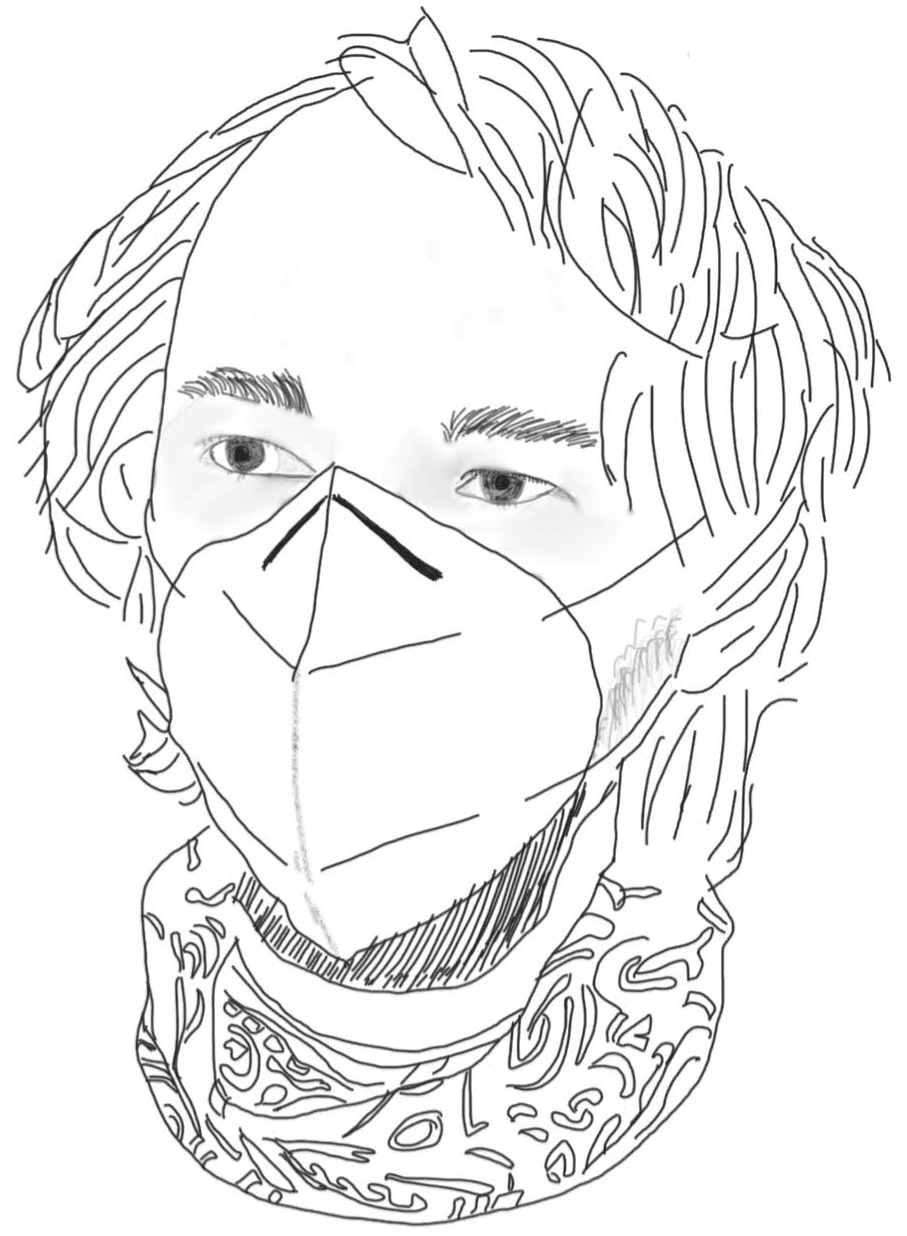
\includegraphics[height=2.5cm]{images/maskavatar-trimmed.jpg}
  \end{minipage}

  \vspace{5mm}
  \noindent
  
\includegraphics[height=1.8cm]{images/payments/qr-btc.pdf}\hspace{0.5cm}%
  
\includegraphics[height=1.8cm]{images/payments/qr-eth.pdf}\hspace{0.5cm}%
  \href{https://paypal.me/ralienpp}{
\includegraphics[height=1.8cm]{images/payments/qr-paypal.pdf}}%
  \hfill
  \href{https://creativecommons.org/licenses/by-sa/4.0/}{\includegraphics[height=0.4cm]{images/cc-by-sa-eps-converted-to.pdf}}
}

\end{document}
"
% ============================================================
%  main-dual.tex — Dual-language edition of
%                  "The Horse, the Dung, and the Car"
%
%  Renders two languages stacked per text block: the PRIMARY language
%  (\booklang) on top, the SECONDARY language (\booklangsecondary) below
%  it in \small\itshape. Body story pages are dual (\dualtr); the cover
%  and the parent-guide prose remain single-language (\tr, primary).
%
%  Languages are configurable. Defaults below: Romanian primary, English
%  secondary. Override from the command line, e.g.:
%    lualatex "\def\booklang{en}\def\booklangsecondary{ro}% !TeX program = lualatex
% !TeX options = -interaction=nonstopmode -halt-on-error "\def\booklang{ro}\def\booklangsecondary{en}\input{main-dual}"
% ============================================================
%  main-dual.tex — Dual-language edition of
%                  "The Horse, the Dung, and the Car"
%
%  Renders two languages stacked per text block: the PRIMARY language
%  (\booklang) on top, the SECONDARY language (\booklangsecondary) below
%  it in \small\itshape. Body story pages are dual (\dualtr); the cover
%  and the parent-guide prose remain single-language (\tr, primary).
%
%  Languages are configurable. Defaults below: Romanian primary, English
%  secondary. Override from the command line, e.g.:
%    lualatex "\def\booklang{en}\def\booklangsecondary{ro}\input{main-dual}"
%
%  Positions differ from main.tex: stacked blocks are taller, so several
%  bottom-anchored text blocks are moved up to keep both languages on the
%  page. main.tex is unchanged.
% ============================================================
\documentclass[17pt]{extarticle}

% --- Language configuration (override before \input to change) ---
\ifdefined\booklang\else\def\booklang{ro}\fi
\ifdefined\booklangsecondary\else\def\booklangsecondary{en}\fi

\def\bookfont{Antykwa Torunska}
%\def\bookfont{OpenDyslexic}
%\def\bookfontpath{fonts/opendyslexic/}
\usepackage[pagenumbers]{picturebook}
\usepackage{multicol}
\usepackage{hyperref}

% Secondary-language styling (optional overrides):
%   \renewcommand{\dualsecstyle}{\small\itshape}
%   \renewcommand{\dualsep}{\par\smallskip}

\begin{document}

% ============================================================
%  COVER (p.1) — modern city   [single language: primary]
% ============================================================
\pagenumbersoff
\singlepage{images/cover.jpeg}{1}{1}{12.8}{%
		\begin{center}
			{\Huge\bfseries \tr{title}}\\[0.5cm]
			{\large \tr{subtitle}}
		\end{center}
}
\block{1}{18}{12.8}{%
	\begin{center}
		{\small \tr{series}}
	\end{center}
}

% ============================================================
%  2x single pp.2–3 — horse tram era
% ============================================================
\pagenumberson
\singlepage{images/modern-city.jpeg}{3.5}{1}{10}{%
	\begin{halo}[color=white, opacity=0.3]
		\dualtr{p01_modern_city}
	\end{halo}
}


\singlepage{images/horse-tram.jpeg}{1}{1}{12.8}{%
	\begin{halo}[color=white, opacity=0.3]
		\dualtr{p02_horse_tram}
	\end{halo}
}

% ============================================================
%  p.4 — growing cities, growing horse population
% ============================================================
\singlepage{images/riders-carriages.jpeg}{1.5}{1}{8}{%
	\begin{halo}[color=white, opacity=0.5]
		\dualtr{p03_growing_cities}
	\end{halo}
}
% moved up (18 -> 15.5) to fit the stacked second language
\block{1}{15.5}{8}{%
	\begin{halo}[color=white, opacity=0.5]
		\dualtr{p03a_more_horses}
	\end{halo}
}

% ============================================================
%  p.5 — New York 1890 statistics
% ============================================================
% moved up (10 -> 8) to fit the stacked subtitle + second language
\singlepage{images/horse-human-pseudotessellation.png}{1}{8}{12.8}{%
	\begin{halo}[color=white, opacity=0.75]
		\dualtr{p04_ny_stats}

		\bigskip
		\dualtr{p04_ny_subtitle}
	\end{halo}
}

% ============================================================
%  SPREAD pp.6–7 — daily horse waste / smell
% ============================================================
\fullspread{images/horse-output.jpeg}%
{1}{1}{12}{% left page
	\begin{halo}[color=white, opacity=0.3]
		\dualtr{p05_manure_stats}

		\bigskip
		\dualtr{p05_subtitle}
	\end{halo}
}%
{2}{1}{10}{% right page — centered question
	\begin{halo}[color=white, opacity=0.3]
		\begin{center}
			{\Large\bfseries \dualtr{p06_smell}}
		\end{center}
	\end{halo}
}

% ============================================================
%  p.8 — alarming situation, people adapting
% ============================================================
\singlepage{images/street-manure.jpeg}{1}{0.5}{12.8}{%
	\begin{halo}[color=white, opacity=0.3]
		\dualtr{p07_alarming}
	\end{halo}
}

% ============================================================
%  p.9 — saved by technology (old car)
% ============================================================
% moved up (18 -> 14.5) — bottom-anchored block grows downward when stacked
\singlepage{images/benz-motorwagen.jpeg}{1}{15}{12.8}{%
	\begin{halo}[color=white, opacity=0.4]
		\dualtr{p08_saved_by_tech}
	\end{halo}
}

% ============================================================
%  SPREAD pp.10–11 — history repeats / growing cars
% ============================================================
\singlepage{images/car-human-pseudotessellation.jpeg}{2}{8}{10}{%
	\begin{halo}[color=yellow, opacity=0.5]
	\begin{center}
		{\Large\bfseries \dualtr{p09_history_repeats}}
	\end{center}
	\end{halo}
}


\singlepage{images/gridlock.jpg}{1}{1}{12}{%
	\begin{halo}[color=white, opacity=0.3]
		\dualtr{p10_cars_growing}
	\end{halo}
}

% ============================================================
%  p.12 — cars produce invisible exhaust
% ============================================================
\singlepage{images/shrouded-in-exhaust-gas-clear.jpeg}{1}{0.8}{12.8}{%
	\begin{halo}[color=white, opacity=0.3]
		\dualtr{p11_exhaust}
	\end{halo}
}

% ============================================================
%  p.13 — can be smelled / detected
% ============================================================
\singlepage{images/shrouded-in-exhaust-gas.jpeg}{1}{0.8}{12.8}{%
	\begin{halo}[color=white, opacity=0.3]
		\dualtr{p12_detect}
	\end{halo}
}

% ============================================================
%  SPREAD pp.14–15 — health effects / piles haven't disappeared
% ============================================================
\fullspread{images/coughing.jpeg}%
{1}{1}{12.8}{% left page
	\begin{halo}[color=white, opacity=0.3]
		\dualtr{p13_health}
	\end{halo}
}%
{2}{1}{10}{% right page — dramatic
	\begin{halo}[color=white, opacity=0.3]
		\begin{center}
			{\Large\bfseries \dualtr{p14_piles_back}}
		\end{center}
	\end{halo}
}

% ============================================================
%  p.16 — what can you do?
% ============================================================
\singlepage{images/what-can-i-do.jpeg}{2}{1}{10}{%
	\begin{halo}[color=white, opacity=0.8]
		\begin{center}
			{\Large\bfseries \dualtr{p15_what_can_you_do}}
		\end{center}
	\end{halo}
}

% ============================================================
%  p.17 — walk, bike, public transport
% ============================================================
\singlepage{images/walk.jpeg}{1}{1}{12.8}{%
		\begin{center}
			\dualtr{p16_walk}
		\end{center}
}


\singlepage{images/cyclists.jpeg}{1}{1}{12.8}{%
		\begin{center}
			\dualtr{p16_bike}
		\end{center}
}

\singlepage{images/train-valley.jpg}{1}{2}{12.8}{%
		\dualtr{p16_public_transport}
}

\singlepage{images/remote-call.jpeg}{1}{1}{12.8}{%
		\begin{center}
			\dualtr{p16_stay}
		\end{center}
}

% ============================================================
%  p.18 — plant a tree
% ============================================================
% moved up (17 -> 15) to fit the stacked second language
\singlepage{images/plant-tree.jpeg}{1}{17}{12.8}{%
		\dualtr{p17_plant_tree}
}

% ============================================================
%  p.19 — use your vote
% ============================================================
\singlepage{images/vote.jpeg}{7}{1}{7}{%
		\dualtr{p18_vote}
}

% ============================================================
%  p.20 — contribute to tech progress
% ============================================================
% moved up (19 -> 16.5) to fit the stacked second language
\singlepage{images/science.jpeg}{1}{16.5}{12.8}{%
	\begin{halo}[color=white, opacity=0.8]
		\dualtr{p19_tech_progress}
	\end{halo}
}


% ============================================================
%  p.21,22 — think about the ecosystem
% ============================================================

\fullspread{images/planet.jpeg}%
{2}{1}{10}{% left page
	\begin{center}
		{\Large\bfseries \dualtr{p20_ecosystem}}
	\end{center}
}%
{2}{1}{10}{% 
	
}

% ============================================================
%  PROSE SECTION — parent guide   [single language: primary]
% ============================================================
\pagenumberson
\pagenumberstyle{center}
\startprose
\section*{\tr{parent_guide_title}}
{\small \tr{parent_guide_body}}

% ============================================================
%  GLOSSARY — vocabulary with IPA and translations
% ============================================================
\ifdefined\bookglossaryoff\else
  \newpage
  \section*{\tr{glossary_title}}

  \printglossary{translations/glossary.csv}{\booklang}{\booklangsecondary}
\fi

% ============================================================
%  BACK COVER
%  Pad to a full saddle-stitch signature (multiple of 4 pages) so
%  the back cover lands on the physical back-cover surface.
% ============================================================
\padbooklet
\backcover{%
  {\noindent\textbf{\tr{other_books_title}}\par\smallskip}
  \begin{bookgrid}
	\book{images/covers/cat-tree.png}{Poetry for kids}
    \book{images/covers/cover-high5.png}{What is software engineering?}
	\book{images/covers/tree-cover.jpeg}{Never give up}
  \end{bookgrid}

  \vfill

  {\noindent\textbf{\tr{about_author_title}}\par\smallskip}
  \noindent
  \begin{minipage}[t]{0.75\textwidth}
    \footnotesize
    \tr{about_author_body}
  \end{minipage}%
  \hfill
  \begin{minipage}[t]{0.2\textwidth}
    \raggedleft
    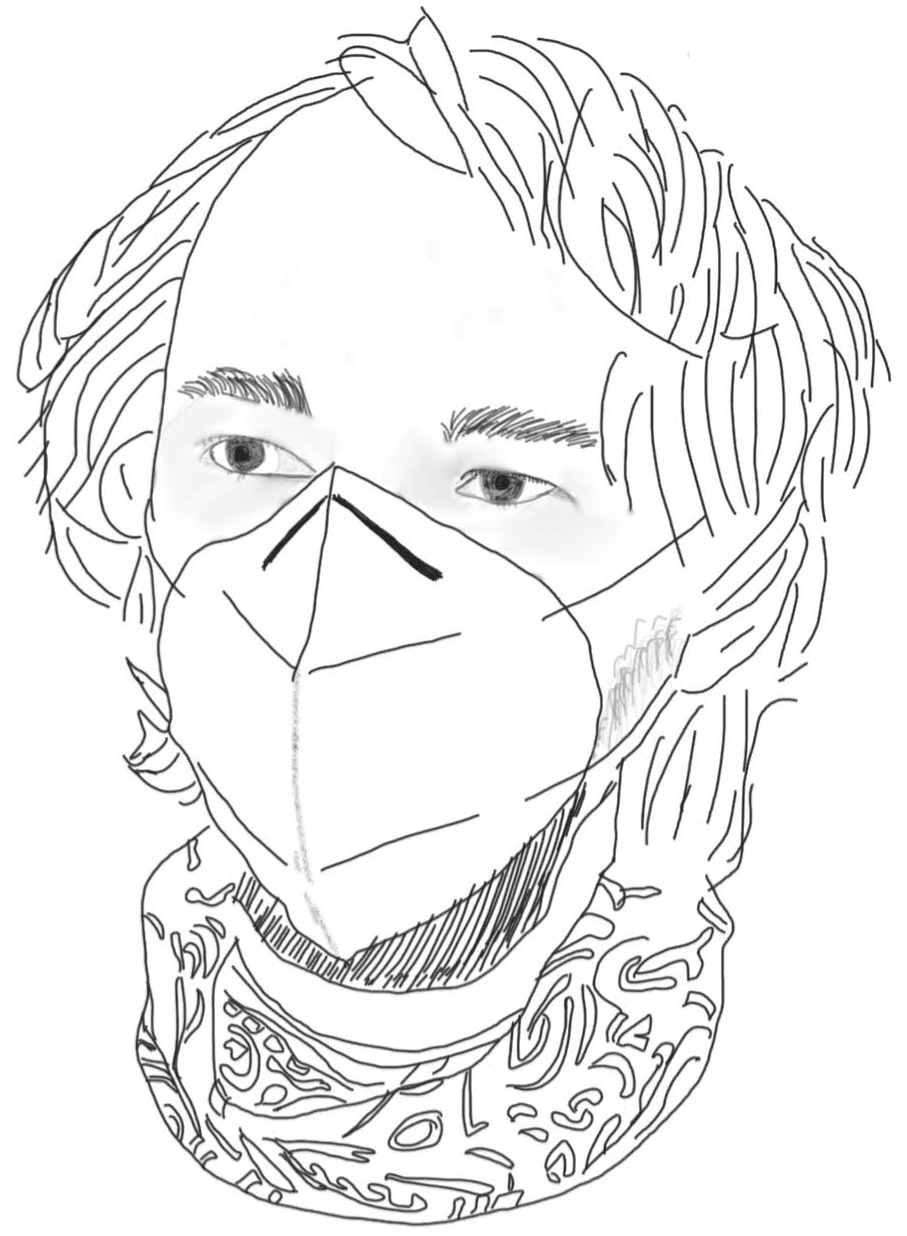
\includegraphics[height=2.5cm]{images/maskavatar-trimmed.jpg}
  \end{minipage}

  \vspace{5mm}
  \noindent
  
\includegraphics[height=1.8cm]{images/payments/qr-btc.pdf}\hspace{0.5cm}%
  
\includegraphics[height=1.8cm]{images/payments/qr-eth.pdf}\hspace{0.5cm}%
  \href{https://paypal.me/ralienpp}{
\includegraphics[height=1.8cm]{images/payments/qr-paypal.pdf}}%
  \hfill
  \href{https://creativecommons.org/licenses/by-sa/4.0/}{\includegraphics[height=0.4cm]{images/cc-by-sa-eps-converted-to.pdf}}
}

\end{document}
"
%
%  Positions differ from main.tex: stacked blocks are taller, so several
%  bottom-anchored text blocks are moved up to keep both languages on the
%  page. main.tex is unchanged.
% ============================================================
\documentclass[17pt]{extarticle}

% --- Language configuration (override before \input to change) ---
\ifdefined\booklang\else\def\booklang{ro}\fi
\ifdefined\booklangsecondary\else\def\booklangsecondary{en}\fi

\def\bookfont{Antykwa Torunska}
%\def\bookfont{OpenDyslexic}
%\def\bookfontpath{fonts/opendyslexic/}
\usepackage[pagenumbers]{picturebook}
\usepackage{multicol}
\usepackage{hyperref}

% Secondary-language styling (optional overrides):
%   \renewcommand{\dualsecstyle}{\small\itshape}
%   \renewcommand{\dualsep}{\par\smallskip}

\begin{document}

% ============================================================
%  COVER (p.1) — modern city   [single language: primary]
% ============================================================
\pagenumbersoff
\singlepage{images/cover.jpeg}{1}{1}{12.8}{%
		\begin{center}
			{\Huge\bfseries \tr{title}}\\[0.5cm]
			{\large \tr{subtitle}}
		\end{center}
}
\block{1}{18}{12.8}{%
	\begin{center}
		{\small \tr{series}}
	\end{center}
}

% ============================================================
%  2x single pp.2–3 — horse tram era
% ============================================================
\pagenumberson
\singlepage{images/modern-city.jpeg}{3.5}{1}{10}{%
	\begin{halo}[color=white, opacity=0.3]
		\dualtr{p01_modern_city}
	\end{halo}
}


\singlepage{images/horse-tram.jpeg}{1}{1}{12.8}{%
	\begin{halo}[color=white, opacity=0.3]
		\dualtr{p02_horse_tram}
	\end{halo}
}

% ============================================================
%  p.4 — growing cities, growing horse population
% ============================================================
\singlepage{images/riders-carriages.jpeg}{1.5}{1}{8}{%
	\begin{halo}[color=white, opacity=0.5]
		\dualtr{p03_growing_cities}
	\end{halo}
}
% moved up (18 -> 15.5) to fit the stacked second language
\block{1}{15.5}{8}{%
	\begin{halo}[color=white, opacity=0.5]
		\dualtr{p03a_more_horses}
	\end{halo}
}

% ============================================================
%  p.5 — New York 1890 statistics
% ============================================================
% moved up (10 -> 8) to fit the stacked subtitle + second language
\singlepage{images/horse-human-pseudotessellation.png}{1}{8}{12.8}{%
	\begin{halo}[color=white, opacity=0.75]
		\dualtr{p04_ny_stats}

		\bigskip
		\dualtr{p04_ny_subtitle}
	\end{halo}
}

% ============================================================
%  SPREAD pp.6–7 — daily horse waste / smell
% ============================================================
\fullspread{images/horse-output.jpeg}%
{1}{1}{12}{% left page
	\begin{halo}[color=white, opacity=0.3]
		\dualtr{p05_manure_stats}

		\bigskip
		\dualtr{p05_subtitle}
	\end{halo}
}%
{2}{1}{10}{% right page — centered question
	\begin{halo}[color=white, opacity=0.3]
		\begin{center}
			{\Large\bfseries \dualtr{p06_smell}}
		\end{center}
	\end{halo}
}

% ============================================================
%  p.8 — alarming situation, people adapting
% ============================================================
\singlepage{images/street-manure.jpeg}{1}{0.5}{12.8}{%
	\begin{halo}[color=white, opacity=0.3]
		\dualtr{p07_alarming}
	\end{halo}
}

% ============================================================
%  p.9 — saved by technology (old car)
% ============================================================
% moved up (18 -> 14.5) — bottom-anchored block grows downward when stacked
\singlepage{images/benz-motorwagen.jpeg}{1}{15}{12.8}{%
	\begin{halo}[color=white, opacity=0.4]
		\dualtr{p08_saved_by_tech}
	\end{halo}
}

% ============================================================
%  SPREAD pp.10–11 — history repeats / growing cars
% ============================================================
\singlepage{images/car-human-pseudotessellation.jpeg}{2}{8}{10}{%
	\begin{halo}[color=yellow, opacity=0.5]
	\begin{center}
		{\Large\bfseries \dualtr{p09_history_repeats}}
	\end{center}
	\end{halo}
}


\singlepage{images/gridlock.jpg}{1}{1}{12}{%
	\begin{halo}[color=white, opacity=0.3]
		\dualtr{p10_cars_growing}
	\end{halo}
}

% ============================================================
%  p.12 — cars produce invisible exhaust
% ============================================================
\singlepage{images/shrouded-in-exhaust-gas-clear.jpeg}{1}{0.8}{12.8}{%
	\begin{halo}[color=white, opacity=0.3]
		\dualtr{p11_exhaust}
	\end{halo}
}

% ============================================================
%  p.13 — can be smelled / detected
% ============================================================
\singlepage{images/shrouded-in-exhaust-gas.jpeg}{1}{0.8}{12.8}{%
	\begin{halo}[color=white, opacity=0.3]
		\dualtr{p12_detect}
	\end{halo}
}

% ============================================================
%  SPREAD pp.14–15 — health effects / piles haven't disappeared
% ============================================================
\fullspread{images/coughing.jpeg}%
{1}{1}{12.8}{% left page
	\begin{halo}[color=white, opacity=0.3]
		\dualtr{p13_health}
	\end{halo}
}%
{2}{1}{10}{% right page — dramatic
	\begin{halo}[color=white, opacity=0.3]
		\begin{center}
			{\Large\bfseries \dualtr{p14_piles_back}}
		\end{center}
	\end{halo}
}

% ============================================================
%  p.16 — what can you do?
% ============================================================
\singlepage{images/what-can-i-do.jpeg}{2}{1}{10}{%
	\begin{halo}[color=white, opacity=0.8]
		\begin{center}
			{\Large\bfseries \dualtr{p15_what_can_you_do}}
		\end{center}
	\end{halo}
}

% ============================================================
%  p.17 — walk, bike, public transport
% ============================================================
\singlepage{images/walk.jpeg}{1}{1}{12.8}{%
		\begin{center}
			\dualtr{p16_walk}
		\end{center}
}


\singlepage{images/cyclists.jpeg}{1}{1}{12.8}{%
		\begin{center}
			\dualtr{p16_bike}
		\end{center}
}

\singlepage{images/train-valley.jpg}{1}{2}{12.8}{%
		\dualtr{p16_public_transport}
}

\singlepage{images/remote-call.jpeg}{1}{1}{12.8}{%
		\begin{center}
			\dualtr{p16_stay}
		\end{center}
}

% ============================================================
%  p.18 — plant a tree
% ============================================================
% moved up (17 -> 15) to fit the stacked second language
\singlepage{images/plant-tree.jpeg}{1}{17}{12.8}{%
		\dualtr{p17_plant_tree}
}

% ============================================================
%  p.19 — use your vote
% ============================================================
\singlepage{images/vote.jpeg}{7}{1}{7}{%
		\dualtr{p18_vote}
}

% ============================================================
%  p.20 — contribute to tech progress
% ============================================================
% moved up (19 -> 16.5) to fit the stacked second language
\singlepage{images/science.jpeg}{1}{16.5}{12.8}{%
	\begin{halo}[color=white, opacity=0.8]
		\dualtr{p19_tech_progress}
	\end{halo}
}


% ============================================================
%  p.21,22 — think about the ecosystem
% ============================================================

\fullspread{images/planet.jpeg}%
{2}{1}{10}{% left page
	\begin{center}
		{\Large\bfseries \dualtr{p20_ecosystem}}
	\end{center}
}%
{2}{1}{10}{% 
	
}

% ============================================================
%  PROSE SECTION — parent guide   [single language: primary]
% ============================================================
\pagenumberson
\pagenumberstyle{center}
\startprose
\section*{\tr{parent_guide_title}}
{\small \tr{parent_guide_body}}

% ============================================================
%  GLOSSARY — vocabulary with IPA and translations
% ============================================================
\ifdefined\bookglossaryoff\else
  \newpage
  \section*{\tr{glossary_title}}

  \printglossary{translations/glossary.csv}{\booklang}{\booklangsecondary}
\fi

% ============================================================
%  BACK COVER
%  Pad to a full saddle-stitch signature (multiple of 4 pages) so
%  the back cover lands on the physical back-cover surface.
% ============================================================
\padbooklet
\backcover{%
  {\noindent\textbf{\tr{other_books_title}}\par\smallskip}
  \begin{bookgrid}
	\book{images/covers/cat-tree.png}{Poetry for kids}
    \book{images/covers/cover-high5.png}{What is software engineering?}
	\book{images/covers/tree-cover.jpeg}{Never give up}
  \end{bookgrid}

  \vfill

  {\noindent\textbf{\tr{about_author_title}}\par\smallskip}
  \noindent
  \begin{minipage}[t]{0.75\textwidth}
    \footnotesize
    \tr{about_author_body}
  \end{minipage}%
  \hfill
  \begin{minipage}[t]{0.2\textwidth}
    \raggedleft
    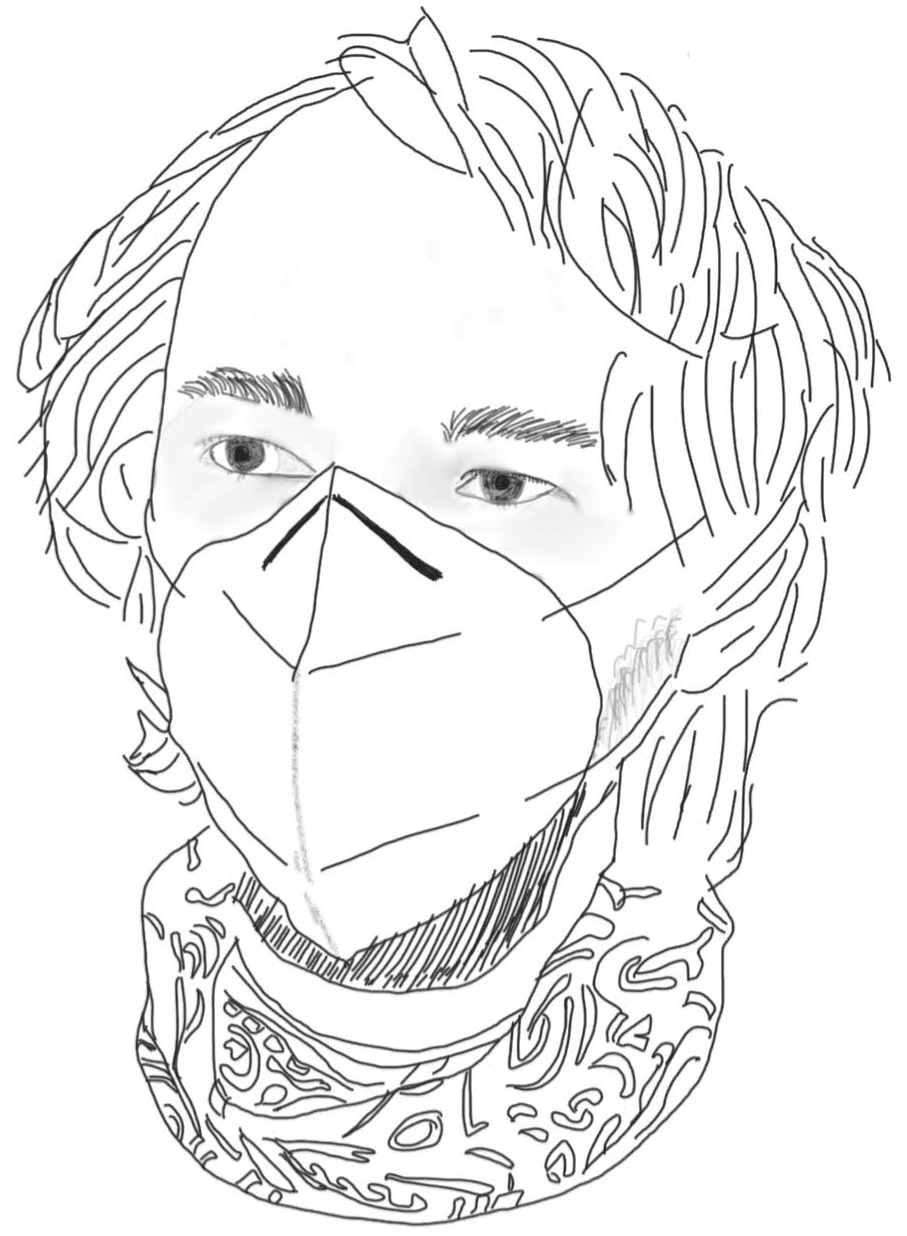
\includegraphics[height=2.5cm]{images/maskavatar-trimmed.jpg}
  \end{minipage}

  \vspace{5mm}
  \noindent
  
\includegraphics[height=1.8cm]{images/payments/qr-btc.pdf}\hspace{0.5cm}%
  
\includegraphics[height=1.8cm]{images/payments/qr-eth.pdf}\hspace{0.5cm}%
  \href{https://paypal.me/ralienpp}{
\includegraphics[height=1.8cm]{images/payments/qr-paypal.pdf}}%
  \hfill
  \href{https://creativecommons.org/licenses/by-sa/4.0/}{\includegraphics[height=0.4cm]{images/cc-by-sa-eps-converted-to.pdf}}
}

\end{document}
"
% ============================================================
%  main-dual.tex — Dual-language edition of
%                  "The Horse, the Dung, and the Car"
%
%  Renders two languages stacked per text block: the PRIMARY language
%  (\booklang) on top, the SECONDARY language (\booklangsecondary) below
%  it in \small\itshape. Body story pages are dual (\dualtr); the cover
%  and the parent-guide prose remain single-language (\tr, primary).
%
%  Languages are configurable. Defaults below: Romanian primary, English
%  secondary. Override from the command line, e.g.:
%    lualatex "\def\booklang{en}\def\booklangsecondary{ro}% !TeX program = lualatex
% !TeX options = -interaction=nonstopmode -halt-on-error "\def\booklang{ro}\def\booklangsecondary{en}% !TeX program = lualatex
% !TeX options = -interaction=nonstopmode -halt-on-error "\def\booklang{ro}\def\booklangsecondary{en}\input{main-dual}"
% ============================================================
%  main-dual.tex — Dual-language edition of
%                  "The Horse, the Dung, and the Car"
%
%  Renders two languages stacked per text block: the PRIMARY language
%  (\booklang) on top, the SECONDARY language (\booklangsecondary) below
%  it in \small\itshape. Body story pages are dual (\dualtr); the cover
%  and the parent-guide prose remain single-language (\tr, primary).
%
%  Languages are configurable. Defaults below: Romanian primary, English
%  secondary. Override from the command line, e.g.:
%    lualatex "\def\booklang{en}\def\booklangsecondary{ro}\input{main-dual}"
%
%  Positions differ from main.tex: stacked blocks are taller, so several
%  bottom-anchored text blocks are moved up to keep both languages on the
%  page. main.tex is unchanged.
% ============================================================
\documentclass[17pt]{extarticle}

% --- Language configuration (override before \input to change) ---
\ifdefined\booklang\else\def\booklang{ro}\fi
\ifdefined\booklangsecondary\else\def\booklangsecondary{en}\fi

\def\bookfont{Antykwa Torunska}
%\def\bookfont{OpenDyslexic}
%\def\bookfontpath{fonts/opendyslexic/}
\usepackage[pagenumbers]{picturebook}
\usepackage{multicol}
\usepackage{hyperref}

% Secondary-language styling (optional overrides):
%   \renewcommand{\dualsecstyle}{\small\itshape}
%   \renewcommand{\dualsep}{\par\smallskip}

\begin{document}

% ============================================================
%  COVER (p.1) — modern city   [single language: primary]
% ============================================================
\pagenumbersoff
\singlepage{images/cover.jpeg}{1}{1}{12.8}{%
		\begin{center}
			{\Huge\bfseries \tr{title}}\\[0.5cm]
			{\large \tr{subtitle}}
		\end{center}
}
\block{1}{18}{12.8}{%
	\begin{center}
		{\small \tr{series}}
	\end{center}
}

% ============================================================
%  2x single pp.2–3 — horse tram era
% ============================================================
\pagenumberson
\singlepage{images/modern-city.jpeg}{3.5}{1}{10}{%
	\begin{halo}[color=white, opacity=0.3]
		\dualtr{p01_modern_city}
	\end{halo}
}


\singlepage{images/horse-tram.jpeg}{1}{1}{12.8}{%
	\begin{halo}[color=white, opacity=0.3]
		\dualtr{p02_horse_tram}
	\end{halo}
}

% ============================================================
%  p.4 — growing cities, growing horse population
% ============================================================
\singlepage{images/riders-carriages.jpeg}{1.5}{1}{8}{%
	\begin{halo}[color=white, opacity=0.5]
		\dualtr{p03_growing_cities}
	\end{halo}
}
% moved up (18 -> 15.5) to fit the stacked second language
\block{1}{15.5}{8}{%
	\begin{halo}[color=white, opacity=0.5]
		\dualtr{p03a_more_horses}
	\end{halo}
}

% ============================================================
%  p.5 — New York 1890 statistics
% ============================================================
% moved up (10 -> 8) to fit the stacked subtitle + second language
\singlepage{images/horse-human-pseudotessellation.png}{1}{8}{12.8}{%
	\begin{halo}[color=white, opacity=0.75]
		\dualtr{p04_ny_stats}

		\bigskip
		\dualtr{p04_ny_subtitle}
	\end{halo}
}

% ============================================================
%  SPREAD pp.6–7 — daily horse waste / smell
% ============================================================
\fullspread{images/horse-output.jpeg}%
{1}{1}{12}{% left page
	\begin{halo}[color=white, opacity=0.3]
		\dualtr{p05_manure_stats}

		\bigskip
		\dualtr{p05_subtitle}
	\end{halo}
}%
{2}{1}{10}{% right page — centered question
	\begin{halo}[color=white, opacity=0.3]
		\begin{center}
			{\Large\bfseries \dualtr{p06_smell}}
		\end{center}
	\end{halo}
}

% ============================================================
%  p.8 — alarming situation, people adapting
% ============================================================
\singlepage{images/street-manure.jpeg}{1}{0.5}{12.8}{%
	\begin{halo}[color=white, opacity=0.3]
		\dualtr{p07_alarming}
	\end{halo}
}

% ============================================================
%  p.9 — saved by technology (old car)
% ============================================================
% moved up (18 -> 14.5) — bottom-anchored block grows downward when stacked
\singlepage{images/benz-motorwagen.jpeg}{1}{15}{12.8}{%
	\begin{halo}[color=white, opacity=0.4]
		\dualtr{p08_saved_by_tech}
	\end{halo}
}

% ============================================================
%  SPREAD pp.10–11 — history repeats / growing cars
% ============================================================
\singlepage{images/car-human-pseudotessellation.jpeg}{2}{8}{10}{%
	\begin{halo}[color=yellow, opacity=0.5]
	\begin{center}
		{\Large\bfseries \dualtr{p09_history_repeats}}
	\end{center}
	\end{halo}
}


\singlepage{images/gridlock.jpg}{1}{1}{12}{%
	\begin{halo}[color=white, opacity=0.3]
		\dualtr{p10_cars_growing}
	\end{halo}
}

% ============================================================
%  p.12 — cars produce invisible exhaust
% ============================================================
\singlepage{images/shrouded-in-exhaust-gas-clear.jpeg}{1}{0.8}{12.8}{%
	\begin{halo}[color=white, opacity=0.3]
		\dualtr{p11_exhaust}
	\end{halo}
}

% ============================================================
%  p.13 — can be smelled / detected
% ============================================================
\singlepage{images/shrouded-in-exhaust-gas.jpeg}{1}{0.8}{12.8}{%
	\begin{halo}[color=white, opacity=0.3]
		\dualtr{p12_detect}
	\end{halo}
}

% ============================================================
%  SPREAD pp.14–15 — health effects / piles haven't disappeared
% ============================================================
\fullspread{images/coughing.jpeg}%
{1}{1}{12.8}{% left page
	\begin{halo}[color=white, opacity=0.3]
		\dualtr{p13_health}
	\end{halo}
}%
{2}{1}{10}{% right page — dramatic
	\begin{halo}[color=white, opacity=0.3]
		\begin{center}
			{\Large\bfseries \dualtr{p14_piles_back}}
		\end{center}
	\end{halo}
}

% ============================================================
%  p.16 — what can you do?
% ============================================================
\singlepage{images/what-can-i-do.jpeg}{2}{1}{10}{%
	\begin{halo}[color=white, opacity=0.8]
		\begin{center}
			{\Large\bfseries \dualtr{p15_what_can_you_do}}
		\end{center}
	\end{halo}
}

% ============================================================
%  p.17 — walk, bike, public transport
% ============================================================
\singlepage{images/walk.jpeg}{1}{1}{12.8}{%
		\begin{center}
			\dualtr{p16_walk}
		\end{center}
}


\singlepage{images/cyclists.jpeg}{1}{1}{12.8}{%
		\begin{center}
			\dualtr{p16_bike}
		\end{center}
}

\singlepage{images/train-valley.jpg}{1}{2}{12.8}{%
		\dualtr{p16_public_transport}
}

\singlepage{images/remote-call.jpeg}{1}{1}{12.8}{%
		\begin{center}
			\dualtr{p16_stay}
		\end{center}
}

% ============================================================
%  p.18 — plant a tree
% ============================================================
% moved up (17 -> 15) to fit the stacked second language
\singlepage{images/plant-tree.jpeg}{1}{17}{12.8}{%
		\dualtr{p17_plant_tree}
}

% ============================================================
%  p.19 — use your vote
% ============================================================
\singlepage{images/vote.jpeg}{7}{1}{7}{%
		\dualtr{p18_vote}
}

% ============================================================
%  p.20 — contribute to tech progress
% ============================================================
% moved up (19 -> 16.5) to fit the stacked second language
\singlepage{images/science.jpeg}{1}{16.5}{12.8}{%
	\begin{halo}[color=white, opacity=0.8]
		\dualtr{p19_tech_progress}
	\end{halo}
}


% ============================================================
%  p.21,22 — think about the ecosystem
% ============================================================

\fullspread{images/planet.jpeg}%
{2}{1}{10}{% left page
	\begin{center}
		{\Large\bfseries \dualtr{p20_ecosystem}}
	\end{center}
}%
{2}{1}{10}{% 
	
}

% ============================================================
%  PROSE SECTION — parent guide   [single language: primary]
% ============================================================
\pagenumberson
\pagenumberstyle{center}
\startprose
\section*{\tr{parent_guide_title}}
{\small \tr{parent_guide_body}}

% ============================================================
%  GLOSSARY — vocabulary with IPA and translations
% ============================================================
\ifdefined\bookglossaryoff\else
  \newpage
  \section*{\tr{glossary_title}}

  \printglossary{translations/glossary.csv}{\booklang}{\booklangsecondary}
\fi

% ============================================================
%  BACK COVER
%  Pad to a full saddle-stitch signature (multiple of 4 pages) so
%  the back cover lands on the physical back-cover surface.
% ============================================================
\padbooklet
\backcover{%
  {\noindent\textbf{\tr{other_books_title}}\par\smallskip}
  \begin{bookgrid}
	\book{images/covers/cat-tree.png}{Poetry for kids}
    \book{images/covers/cover-high5.png}{What is software engineering?}
	\book{images/covers/tree-cover.jpeg}{Never give up}
  \end{bookgrid}

  \vfill

  {\noindent\textbf{\tr{about_author_title}}\par\smallskip}
  \noindent
  \begin{minipage}[t]{0.75\textwidth}
    \footnotesize
    \tr{about_author_body}
  \end{minipage}%
  \hfill
  \begin{minipage}[t]{0.2\textwidth}
    \raggedleft
    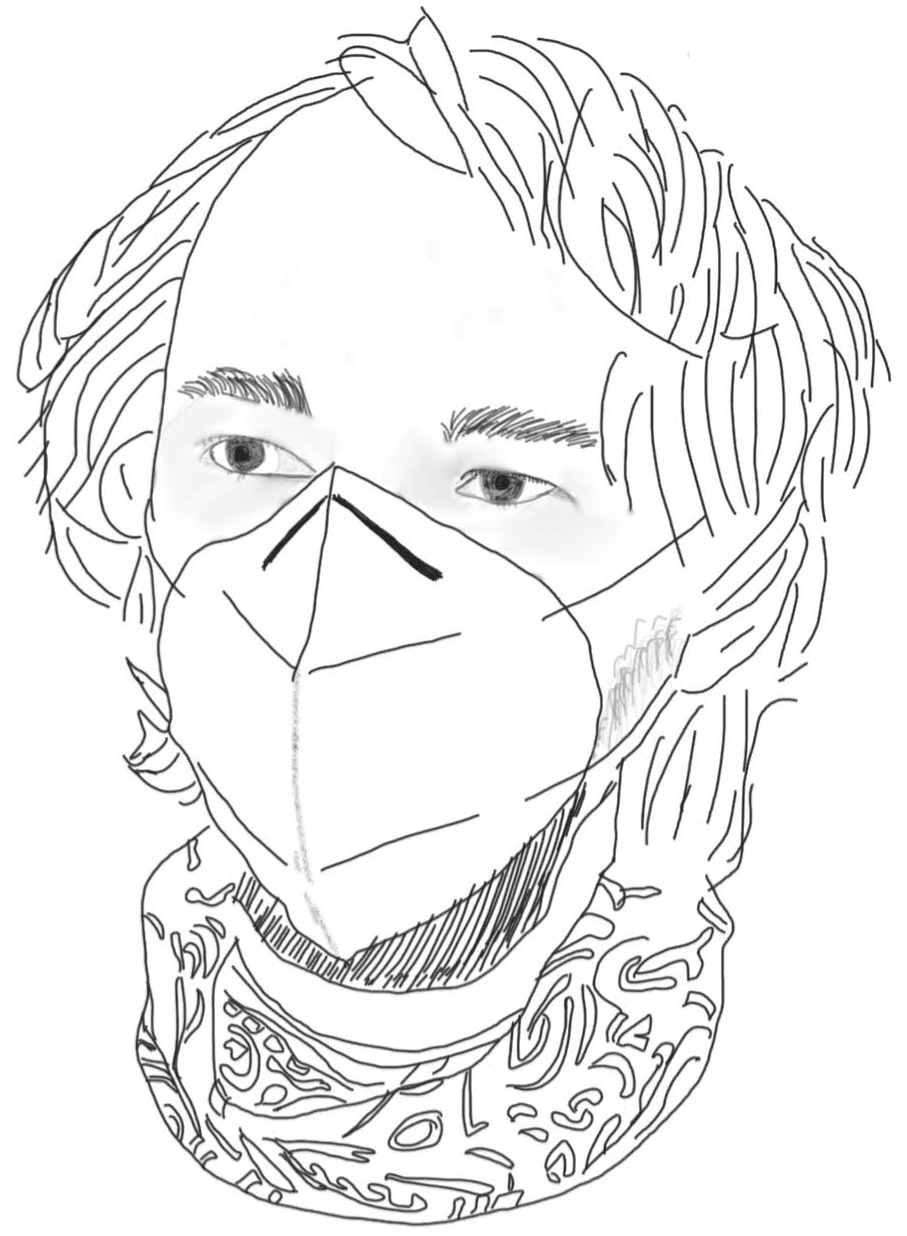
\includegraphics[height=2.5cm]{images/maskavatar-trimmed.jpg}
  \end{minipage}

  \vspace{5mm}
  \noindent
  
\includegraphics[height=1.8cm]{images/payments/qr-btc.pdf}\hspace{0.5cm}%
  
\includegraphics[height=1.8cm]{images/payments/qr-eth.pdf}\hspace{0.5cm}%
  \href{https://paypal.me/ralienpp}{
\includegraphics[height=1.8cm]{images/payments/qr-paypal.pdf}}%
  \hfill
  \href{https://creativecommons.org/licenses/by-sa/4.0/}{\includegraphics[height=0.4cm]{images/cc-by-sa-eps-converted-to.pdf}}
}

\end{document}
"
% ============================================================
%  main-dual.tex — Dual-language edition of
%                  "The Horse, the Dung, and the Car"
%
%  Renders two languages stacked per text block: the PRIMARY language
%  (\booklang) on top, the SECONDARY language (\booklangsecondary) below
%  it in \small\itshape. Body story pages are dual (\dualtr); the cover
%  and the parent-guide prose remain single-language (\tr, primary).
%
%  Languages are configurable. Defaults below: Romanian primary, English
%  secondary. Override from the command line, e.g.:
%    lualatex "\def\booklang{en}\def\booklangsecondary{ro}% !TeX program = lualatex
% !TeX options = -interaction=nonstopmode -halt-on-error "\def\booklang{ro}\def\booklangsecondary{en}\input{main-dual}"
% ============================================================
%  main-dual.tex — Dual-language edition of
%                  "The Horse, the Dung, and the Car"
%
%  Renders two languages stacked per text block: the PRIMARY language
%  (\booklang) on top, the SECONDARY language (\booklangsecondary) below
%  it in \small\itshape. Body story pages are dual (\dualtr); the cover
%  and the parent-guide prose remain single-language (\tr, primary).
%
%  Languages are configurable. Defaults below: Romanian primary, English
%  secondary. Override from the command line, e.g.:
%    lualatex "\def\booklang{en}\def\booklangsecondary{ro}\input{main-dual}"
%
%  Positions differ from main.tex: stacked blocks are taller, so several
%  bottom-anchored text blocks are moved up to keep both languages on the
%  page. main.tex is unchanged.
% ============================================================
\documentclass[17pt]{extarticle}

% --- Language configuration (override before \input to change) ---
\ifdefined\booklang\else\def\booklang{ro}\fi
\ifdefined\booklangsecondary\else\def\booklangsecondary{en}\fi

\def\bookfont{Antykwa Torunska}
%\def\bookfont{OpenDyslexic}
%\def\bookfontpath{fonts/opendyslexic/}
\usepackage[pagenumbers]{picturebook}
\usepackage{multicol}
\usepackage{hyperref}

% Secondary-language styling (optional overrides):
%   \renewcommand{\dualsecstyle}{\small\itshape}
%   \renewcommand{\dualsep}{\par\smallskip}

\begin{document}

% ============================================================
%  COVER (p.1) — modern city   [single language: primary]
% ============================================================
\pagenumbersoff
\singlepage{images/cover.jpeg}{1}{1}{12.8}{%
		\begin{center}
			{\Huge\bfseries \tr{title}}\\[0.5cm]
			{\large \tr{subtitle}}
		\end{center}
}
\block{1}{18}{12.8}{%
	\begin{center}
		{\small \tr{series}}
	\end{center}
}

% ============================================================
%  2x single pp.2–3 — horse tram era
% ============================================================
\pagenumberson
\singlepage{images/modern-city.jpeg}{3.5}{1}{10}{%
	\begin{halo}[color=white, opacity=0.3]
		\dualtr{p01_modern_city}
	\end{halo}
}


\singlepage{images/horse-tram.jpeg}{1}{1}{12.8}{%
	\begin{halo}[color=white, opacity=0.3]
		\dualtr{p02_horse_tram}
	\end{halo}
}

% ============================================================
%  p.4 — growing cities, growing horse population
% ============================================================
\singlepage{images/riders-carriages.jpeg}{1.5}{1}{8}{%
	\begin{halo}[color=white, opacity=0.5]
		\dualtr{p03_growing_cities}
	\end{halo}
}
% moved up (18 -> 15.5) to fit the stacked second language
\block{1}{15.5}{8}{%
	\begin{halo}[color=white, opacity=0.5]
		\dualtr{p03a_more_horses}
	\end{halo}
}

% ============================================================
%  p.5 — New York 1890 statistics
% ============================================================
% moved up (10 -> 8) to fit the stacked subtitle + second language
\singlepage{images/horse-human-pseudotessellation.png}{1}{8}{12.8}{%
	\begin{halo}[color=white, opacity=0.75]
		\dualtr{p04_ny_stats}

		\bigskip
		\dualtr{p04_ny_subtitle}
	\end{halo}
}

% ============================================================
%  SPREAD pp.6–7 — daily horse waste / smell
% ============================================================
\fullspread{images/horse-output.jpeg}%
{1}{1}{12}{% left page
	\begin{halo}[color=white, opacity=0.3]
		\dualtr{p05_manure_stats}

		\bigskip
		\dualtr{p05_subtitle}
	\end{halo}
}%
{2}{1}{10}{% right page — centered question
	\begin{halo}[color=white, opacity=0.3]
		\begin{center}
			{\Large\bfseries \dualtr{p06_smell}}
		\end{center}
	\end{halo}
}

% ============================================================
%  p.8 — alarming situation, people adapting
% ============================================================
\singlepage{images/street-manure.jpeg}{1}{0.5}{12.8}{%
	\begin{halo}[color=white, opacity=0.3]
		\dualtr{p07_alarming}
	\end{halo}
}

% ============================================================
%  p.9 — saved by technology (old car)
% ============================================================
% moved up (18 -> 14.5) — bottom-anchored block grows downward when stacked
\singlepage{images/benz-motorwagen.jpeg}{1}{15}{12.8}{%
	\begin{halo}[color=white, opacity=0.4]
		\dualtr{p08_saved_by_tech}
	\end{halo}
}

% ============================================================
%  SPREAD pp.10–11 — history repeats / growing cars
% ============================================================
\singlepage{images/car-human-pseudotessellation.jpeg}{2}{8}{10}{%
	\begin{halo}[color=yellow, opacity=0.5]
	\begin{center}
		{\Large\bfseries \dualtr{p09_history_repeats}}
	\end{center}
	\end{halo}
}


\singlepage{images/gridlock.jpg}{1}{1}{12}{%
	\begin{halo}[color=white, opacity=0.3]
		\dualtr{p10_cars_growing}
	\end{halo}
}

% ============================================================
%  p.12 — cars produce invisible exhaust
% ============================================================
\singlepage{images/shrouded-in-exhaust-gas-clear.jpeg}{1}{0.8}{12.8}{%
	\begin{halo}[color=white, opacity=0.3]
		\dualtr{p11_exhaust}
	\end{halo}
}

% ============================================================
%  p.13 — can be smelled / detected
% ============================================================
\singlepage{images/shrouded-in-exhaust-gas.jpeg}{1}{0.8}{12.8}{%
	\begin{halo}[color=white, opacity=0.3]
		\dualtr{p12_detect}
	\end{halo}
}

% ============================================================
%  SPREAD pp.14–15 — health effects / piles haven't disappeared
% ============================================================
\fullspread{images/coughing.jpeg}%
{1}{1}{12.8}{% left page
	\begin{halo}[color=white, opacity=0.3]
		\dualtr{p13_health}
	\end{halo}
}%
{2}{1}{10}{% right page — dramatic
	\begin{halo}[color=white, opacity=0.3]
		\begin{center}
			{\Large\bfseries \dualtr{p14_piles_back}}
		\end{center}
	\end{halo}
}

% ============================================================
%  p.16 — what can you do?
% ============================================================
\singlepage{images/what-can-i-do.jpeg}{2}{1}{10}{%
	\begin{halo}[color=white, opacity=0.8]
		\begin{center}
			{\Large\bfseries \dualtr{p15_what_can_you_do}}
		\end{center}
	\end{halo}
}

% ============================================================
%  p.17 — walk, bike, public transport
% ============================================================
\singlepage{images/walk.jpeg}{1}{1}{12.8}{%
		\begin{center}
			\dualtr{p16_walk}
		\end{center}
}


\singlepage{images/cyclists.jpeg}{1}{1}{12.8}{%
		\begin{center}
			\dualtr{p16_bike}
		\end{center}
}

\singlepage{images/train-valley.jpg}{1}{2}{12.8}{%
		\dualtr{p16_public_transport}
}

\singlepage{images/remote-call.jpeg}{1}{1}{12.8}{%
		\begin{center}
			\dualtr{p16_stay}
		\end{center}
}

% ============================================================
%  p.18 — plant a tree
% ============================================================
% moved up (17 -> 15) to fit the stacked second language
\singlepage{images/plant-tree.jpeg}{1}{17}{12.8}{%
		\dualtr{p17_plant_tree}
}

% ============================================================
%  p.19 — use your vote
% ============================================================
\singlepage{images/vote.jpeg}{7}{1}{7}{%
		\dualtr{p18_vote}
}

% ============================================================
%  p.20 — contribute to tech progress
% ============================================================
% moved up (19 -> 16.5) to fit the stacked second language
\singlepage{images/science.jpeg}{1}{16.5}{12.8}{%
	\begin{halo}[color=white, opacity=0.8]
		\dualtr{p19_tech_progress}
	\end{halo}
}


% ============================================================
%  p.21,22 — think about the ecosystem
% ============================================================

\fullspread{images/planet.jpeg}%
{2}{1}{10}{% left page
	\begin{center}
		{\Large\bfseries \dualtr{p20_ecosystem}}
	\end{center}
}%
{2}{1}{10}{% 
	
}

% ============================================================
%  PROSE SECTION — parent guide   [single language: primary]
% ============================================================
\pagenumberson
\pagenumberstyle{center}
\startprose
\section*{\tr{parent_guide_title}}
{\small \tr{parent_guide_body}}

% ============================================================
%  GLOSSARY — vocabulary with IPA and translations
% ============================================================
\ifdefined\bookglossaryoff\else
  \newpage
  \section*{\tr{glossary_title}}

  \printglossary{translations/glossary.csv}{\booklang}{\booklangsecondary}
\fi

% ============================================================
%  BACK COVER
%  Pad to a full saddle-stitch signature (multiple of 4 pages) so
%  the back cover lands on the physical back-cover surface.
% ============================================================
\padbooklet
\backcover{%
  {\noindent\textbf{\tr{other_books_title}}\par\smallskip}
  \begin{bookgrid}
	\book{images/covers/cat-tree.png}{Poetry for kids}
    \book{images/covers/cover-high5.png}{What is software engineering?}
	\book{images/covers/tree-cover.jpeg}{Never give up}
  \end{bookgrid}

  \vfill

  {\noindent\textbf{\tr{about_author_title}}\par\smallskip}
  \noindent
  \begin{minipage}[t]{0.75\textwidth}
    \footnotesize
    \tr{about_author_body}
  \end{minipage}%
  \hfill
  \begin{minipage}[t]{0.2\textwidth}
    \raggedleft
    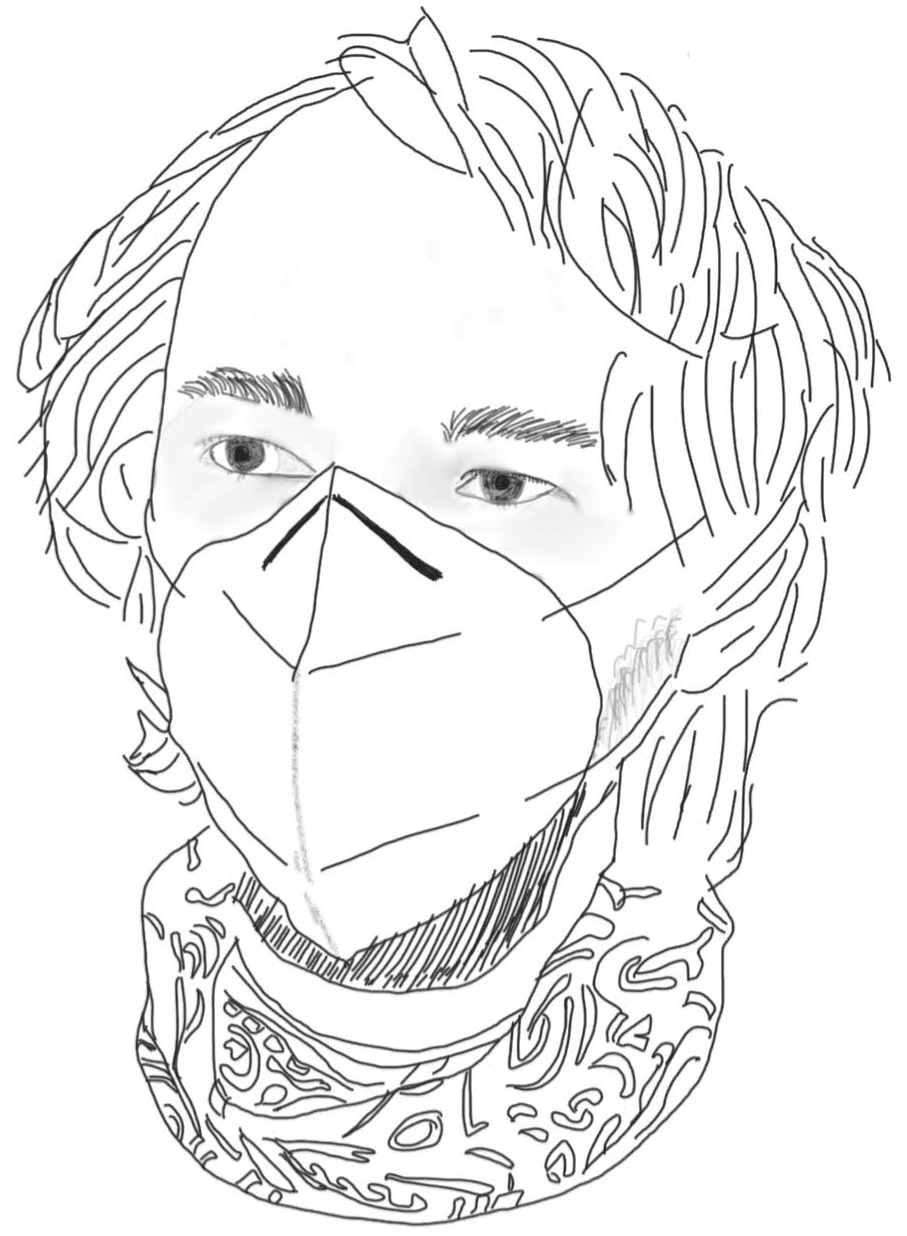
\includegraphics[height=2.5cm]{images/maskavatar-trimmed.jpg}
  \end{minipage}

  \vspace{5mm}
  \noindent
  
\includegraphics[height=1.8cm]{images/payments/qr-btc.pdf}\hspace{0.5cm}%
  
\includegraphics[height=1.8cm]{images/payments/qr-eth.pdf}\hspace{0.5cm}%
  \href{https://paypal.me/ralienpp}{
\includegraphics[height=1.8cm]{images/payments/qr-paypal.pdf}}%
  \hfill
  \href{https://creativecommons.org/licenses/by-sa/4.0/}{\includegraphics[height=0.4cm]{images/cc-by-sa-eps-converted-to.pdf}}
}

\end{document}
"
%
%  Positions differ from main.tex: stacked blocks are taller, so several
%  bottom-anchored text blocks are moved up to keep both languages on the
%  page. main.tex is unchanged.
% ============================================================
\documentclass[17pt]{extarticle}

% --- Language configuration (override before \input to change) ---
\ifdefined\booklang\else\def\booklang{ro}\fi
\ifdefined\booklangsecondary\else\def\booklangsecondary{en}\fi

\def\bookfont{Antykwa Torunska}
%\def\bookfont{OpenDyslexic}
%\def\bookfontpath{fonts/opendyslexic/}
\usepackage[pagenumbers]{picturebook}
\usepackage{multicol}
\usepackage{hyperref}

% Secondary-language styling (optional overrides):
%   \renewcommand{\dualsecstyle}{\small\itshape}
%   \renewcommand{\dualsep}{\par\smallskip}

\begin{document}

% ============================================================
%  COVER (p.1) — modern city   [single language: primary]
% ============================================================
\pagenumbersoff
\singlepage{images/cover.jpeg}{1}{1}{12.8}{%
		\begin{center}
			{\Huge\bfseries \tr{title}}\\[0.5cm]
			{\large \tr{subtitle}}
		\end{center}
}
\block{1}{18}{12.8}{%
	\begin{center}
		{\small \tr{series}}
	\end{center}
}

% ============================================================
%  2x single pp.2–3 — horse tram era
% ============================================================
\pagenumberson
\singlepage{images/modern-city.jpeg}{3.5}{1}{10}{%
	\begin{halo}[color=white, opacity=0.3]
		\dualtr{p01_modern_city}
	\end{halo}
}


\singlepage{images/horse-tram.jpeg}{1}{1}{12.8}{%
	\begin{halo}[color=white, opacity=0.3]
		\dualtr{p02_horse_tram}
	\end{halo}
}

% ============================================================
%  p.4 — growing cities, growing horse population
% ============================================================
\singlepage{images/riders-carriages.jpeg}{1.5}{1}{8}{%
	\begin{halo}[color=white, opacity=0.5]
		\dualtr{p03_growing_cities}
	\end{halo}
}
% moved up (18 -> 15.5) to fit the stacked second language
\block{1}{15.5}{8}{%
	\begin{halo}[color=white, opacity=0.5]
		\dualtr{p03a_more_horses}
	\end{halo}
}

% ============================================================
%  p.5 — New York 1890 statistics
% ============================================================
% moved up (10 -> 8) to fit the stacked subtitle + second language
\singlepage{images/horse-human-pseudotessellation.png}{1}{8}{12.8}{%
	\begin{halo}[color=white, opacity=0.75]
		\dualtr{p04_ny_stats}

		\bigskip
		\dualtr{p04_ny_subtitle}
	\end{halo}
}

% ============================================================
%  SPREAD pp.6–7 — daily horse waste / smell
% ============================================================
\fullspread{images/horse-output.jpeg}%
{1}{1}{12}{% left page
	\begin{halo}[color=white, opacity=0.3]
		\dualtr{p05_manure_stats}

		\bigskip
		\dualtr{p05_subtitle}
	\end{halo}
}%
{2}{1}{10}{% right page — centered question
	\begin{halo}[color=white, opacity=0.3]
		\begin{center}
			{\Large\bfseries \dualtr{p06_smell}}
		\end{center}
	\end{halo}
}

% ============================================================
%  p.8 — alarming situation, people adapting
% ============================================================
\singlepage{images/street-manure.jpeg}{1}{0.5}{12.8}{%
	\begin{halo}[color=white, opacity=0.3]
		\dualtr{p07_alarming}
	\end{halo}
}

% ============================================================
%  p.9 — saved by technology (old car)
% ============================================================
% moved up (18 -> 14.5) — bottom-anchored block grows downward when stacked
\singlepage{images/benz-motorwagen.jpeg}{1}{15}{12.8}{%
	\begin{halo}[color=white, opacity=0.4]
		\dualtr{p08_saved_by_tech}
	\end{halo}
}

% ============================================================
%  SPREAD pp.10–11 — history repeats / growing cars
% ============================================================
\singlepage{images/car-human-pseudotessellation.jpeg}{2}{8}{10}{%
	\begin{halo}[color=yellow, opacity=0.5]
	\begin{center}
		{\Large\bfseries \dualtr{p09_history_repeats}}
	\end{center}
	\end{halo}
}


\singlepage{images/gridlock.jpg}{1}{1}{12}{%
	\begin{halo}[color=white, opacity=0.3]
		\dualtr{p10_cars_growing}
	\end{halo}
}

% ============================================================
%  p.12 — cars produce invisible exhaust
% ============================================================
\singlepage{images/shrouded-in-exhaust-gas-clear.jpeg}{1}{0.8}{12.8}{%
	\begin{halo}[color=white, opacity=0.3]
		\dualtr{p11_exhaust}
	\end{halo}
}

% ============================================================
%  p.13 — can be smelled / detected
% ============================================================
\singlepage{images/shrouded-in-exhaust-gas.jpeg}{1}{0.8}{12.8}{%
	\begin{halo}[color=white, opacity=0.3]
		\dualtr{p12_detect}
	\end{halo}
}

% ============================================================
%  SPREAD pp.14–15 — health effects / piles haven't disappeared
% ============================================================
\fullspread{images/coughing.jpeg}%
{1}{1}{12.8}{% left page
	\begin{halo}[color=white, opacity=0.3]
		\dualtr{p13_health}
	\end{halo}
}%
{2}{1}{10}{% right page — dramatic
	\begin{halo}[color=white, opacity=0.3]
		\begin{center}
			{\Large\bfseries \dualtr{p14_piles_back}}
		\end{center}
	\end{halo}
}

% ============================================================
%  p.16 — what can you do?
% ============================================================
\singlepage{images/what-can-i-do.jpeg}{2}{1}{10}{%
	\begin{halo}[color=white, opacity=0.8]
		\begin{center}
			{\Large\bfseries \dualtr{p15_what_can_you_do}}
		\end{center}
	\end{halo}
}

% ============================================================
%  p.17 — walk, bike, public transport
% ============================================================
\singlepage{images/walk.jpeg}{1}{1}{12.8}{%
		\begin{center}
			\dualtr{p16_walk}
		\end{center}
}


\singlepage{images/cyclists.jpeg}{1}{1}{12.8}{%
		\begin{center}
			\dualtr{p16_bike}
		\end{center}
}

\singlepage{images/train-valley.jpg}{1}{2}{12.8}{%
		\dualtr{p16_public_transport}
}

\singlepage{images/remote-call.jpeg}{1}{1}{12.8}{%
		\begin{center}
			\dualtr{p16_stay}
		\end{center}
}

% ============================================================
%  p.18 — plant a tree
% ============================================================
% moved up (17 -> 15) to fit the stacked second language
\singlepage{images/plant-tree.jpeg}{1}{17}{12.8}{%
		\dualtr{p17_plant_tree}
}

% ============================================================
%  p.19 — use your vote
% ============================================================
\singlepage{images/vote.jpeg}{7}{1}{7}{%
		\dualtr{p18_vote}
}

% ============================================================
%  p.20 — contribute to tech progress
% ============================================================
% moved up (19 -> 16.5) to fit the stacked second language
\singlepage{images/science.jpeg}{1}{16.5}{12.8}{%
	\begin{halo}[color=white, opacity=0.8]
		\dualtr{p19_tech_progress}
	\end{halo}
}


% ============================================================
%  p.21,22 — think about the ecosystem
% ============================================================

\fullspread{images/planet.jpeg}%
{2}{1}{10}{% left page
	\begin{center}
		{\Large\bfseries \dualtr{p20_ecosystem}}
	\end{center}
}%
{2}{1}{10}{% 
	
}

% ============================================================
%  PROSE SECTION — parent guide   [single language: primary]
% ============================================================
\pagenumberson
\pagenumberstyle{center}
\startprose
\section*{\tr{parent_guide_title}}
{\small \tr{parent_guide_body}}

% ============================================================
%  GLOSSARY — vocabulary with IPA and translations
% ============================================================
\ifdefined\bookglossaryoff\else
  \newpage
  \section*{\tr{glossary_title}}

  \printglossary{translations/glossary.csv}{\booklang}{\booklangsecondary}
\fi

% ============================================================
%  BACK COVER
%  Pad to a full saddle-stitch signature (multiple of 4 pages) so
%  the back cover lands on the physical back-cover surface.
% ============================================================
\padbooklet
\backcover{%
  {\noindent\textbf{\tr{other_books_title}}\par\smallskip}
  \begin{bookgrid}
	\book{images/covers/cat-tree.png}{Poetry for kids}
    \book{images/covers/cover-high5.png}{What is software engineering?}
	\book{images/covers/tree-cover.jpeg}{Never give up}
  \end{bookgrid}

  \vfill

  {\noindent\textbf{\tr{about_author_title}}\par\smallskip}
  \noindent
  \begin{minipage}[t]{0.75\textwidth}
    \footnotesize
    \tr{about_author_body}
  \end{minipage}%
  \hfill
  \begin{minipage}[t]{0.2\textwidth}
    \raggedleft
    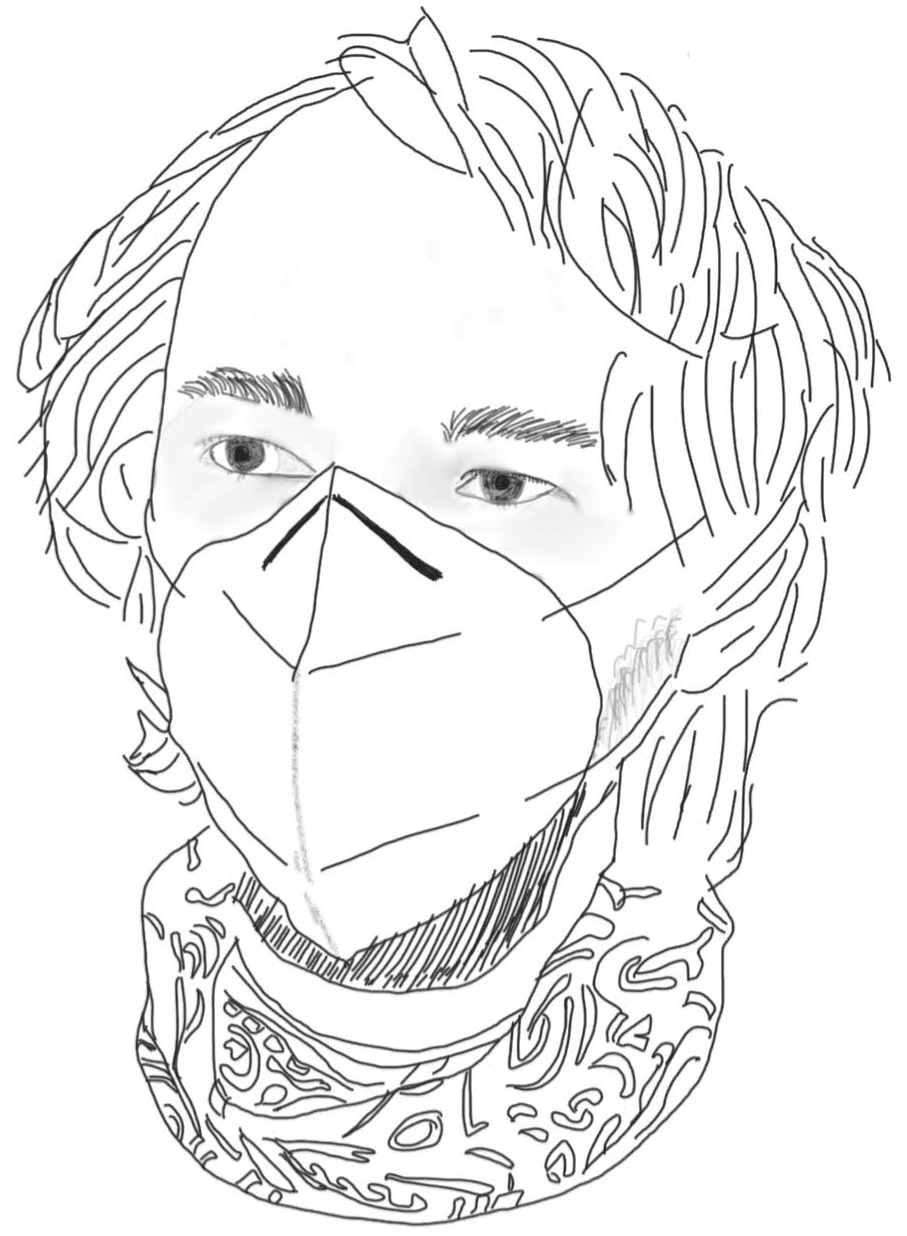
\includegraphics[height=2.5cm]{images/maskavatar-trimmed.jpg}
  \end{minipage}

  \vspace{5mm}
  \noindent
  
\includegraphics[height=1.8cm]{images/payments/qr-btc.pdf}\hspace{0.5cm}%
  
\includegraphics[height=1.8cm]{images/payments/qr-eth.pdf}\hspace{0.5cm}%
  \href{https://paypal.me/ralienpp}{
\includegraphics[height=1.8cm]{images/payments/qr-paypal.pdf}}%
  \hfill
  \href{https://creativecommons.org/licenses/by-sa/4.0/}{\includegraphics[height=0.4cm]{images/cc-by-sa-eps-converted-to.pdf}}
}

\end{document}
"
%
%  Positions differ from main.tex: stacked blocks are taller, so several
%  bottom-anchored text blocks are moved up to keep both languages on the
%  page. main.tex is unchanged.
% ============================================================
\documentclass[17pt]{extarticle}

% --- Language configuration (override before \input to change) ---
\ifdefined\booklang\else\def\booklang{ro}\fi
\ifdefined\booklangsecondary\else\def\booklangsecondary{en}\fi

\def\bookfont{Antykwa Torunska}
%\def\bookfont{OpenDyslexic}
%\def\bookfontpath{fonts/opendyslexic/}
\usepackage[pagenumbers]{picturebook}
\usepackage{multicol}
\usepackage{hyperref}

% Secondary-language styling (optional overrides):
%   \renewcommand{\dualsecstyle}{\small\itshape}
%   \renewcommand{\dualsep}{\par\smallskip}

\begin{document}

% ============================================================
%  COVER (p.1) — modern city   [single language: primary]
% ============================================================
\pagenumbersoff
\singlepage{images/cover.jpeg}{1}{1}{12.8}{%
		\begin{center}
			{\Huge\bfseries \tr{title}}\\[0.5cm]
			{\large \tr{subtitle}}
		\end{center}
}
\block{1}{18}{12.8}{%
	\begin{center}
		{\small \tr{series}}
	\end{center}
}

% ============================================================
%  2x single pp.2–3 — horse tram era
% ============================================================
\pagenumberson
\singlepage{images/modern-city.jpeg}{3.5}{1}{10}{%
	\begin{halo}[color=white, opacity=0.3]
		\dualtr{p01_modern_city}
	\end{halo}
}


\singlepage{images/horse-tram.jpeg}{1}{1}{12.8}{%
	\begin{halo}[color=white, opacity=0.3]
		\dualtr{p02_horse_tram}
	\end{halo}
}

% ============================================================
%  p.4 — growing cities, growing horse population
% ============================================================
\singlepage{images/riders-carriages.jpeg}{1.5}{1}{8}{%
	\begin{halo}[color=white, opacity=0.5]
		\dualtr{p03_growing_cities}
	\end{halo}
}
% moved up (18 -> 15.5) to fit the stacked second language
\block{1}{15.5}{8}{%
	\begin{halo}[color=white, opacity=0.5]
		\dualtr{p03a_more_horses}
	\end{halo}
}

% ============================================================
%  p.5 — New York 1890 statistics
% ============================================================
% moved up (10 -> 8) to fit the stacked subtitle + second language
\singlepage{images/horse-human-pseudotessellation.png}{1}{8}{12.8}{%
	\begin{halo}[color=white, opacity=0.75]
		\dualtr{p04_ny_stats}

		\bigskip
		\dualtr{p04_ny_subtitle}
	\end{halo}
}

% ============================================================
%  SPREAD pp.6–7 — daily horse waste / smell
% ============================================================
\fullspread{images/horse-output.jpeg}%
{1}{1}{12}{% left page
	\begin{halo}[color=white, opacity=0.3]
		\dualtr{p05_manure_stats}

		\bigskip
		\dualtr{p05_subtitle}
	\end{halo}
}%
{2}{1}{10}{% right page — centered question
	\begin{halo}[color=white, opacity=0.3]
		\begin{center}
			{\Large\bfseries \dualtr{p06_smell}}
		\end{center}
	\end{halo}
}

% ============================================================
%  p.8 — alarming situation, people adapting
% ============================================================
\singlepage{images/street-manure.jpeg}{1}{0.5}{12.8}{%
	\begin{halo}[color=white, opacity=0.3]
		\dualtr{p07_alarming}
	\end{halo}
}

% ============================================================
%  p.9 — saved by technology (old car)
% ============================================================
% moved up (18 -> 14.5) — bottom-anchored block grows downward when stacked
\singlepage{images/benz-motorwagen.jpeg}{1}{15}{12.8}{%
	\begin{halo}[color=white, opacity=0.4]
		\dualtr{p08_saved_by_tech}
	\end{halo}
}

% ============================================================
%  SPREAD pp.10–11 — history repeats / growing cars
% ============================================================
\singlepage{images/car-human-pseudotessellation.jpeg}{2}{8}{10}{%
	\begin{halo}[color=yellow, opacity=0.5]
	\begin{center}
		{\Large\bfseries \dualtr{p09_history_repeats}}
	\end{center}
	\end{halo}
}


\singlepage{images/gridlock.jpg}{1}{1}{12}{%
	\begin{halo}[color=white, opacity=0.3]
		\dualtr{p10_cars_growing}
	\end{halo}
}

% ============================================================
%  p.12 — cars produce invisible exhaust
% ============================================================
\singlepage{images/shrouded-in-exhaust-gas-clear.jpeg}{1}{0.8}{12.8}{%
	\begin{halo}[color=white, opacity=0.3]
		\dualtr{p11_exhaust}
	\end{halo}
}

% ============================================================
%  p.13 — can be smelled / detected
% ============================================================
\singlepage{images/shrouded-in-exhaust-gas.jpeg}{1}{0.8}{12.8}{%
	\begin{halo}[color=white, opacity=0.3]
		\dualtr{p12_detect}
	\end{halo}
}

% ============================================================
%  SPREAD pp.14–15 — health effects / piles haven't disappeared
% ============================================================
\fullspread{images/coughing.jpeg}%
{1}{1}{12.8}{% left page
	\begin{halo}[color=white, opacity=0.3]
		\dualtr{p13_health}
	\end{halo}
}%
{2}{1}{10}{% right page — dramatic
	\begin{halo}[color=white, opacity=0.3]
		\begin{center}
			{\Large\bfseries \dualtr{p14_piles_back}}
		\end{center}
	\end{halo}
}

% ============================================================
%  p.16 — what can you do?
% ============================================================
\singlepage{images/what-can-i-do.jpeg}{2}{1}{10}{%
	\begin{halo}[color=white, opacity=0.8]
		\begin{center}
			{\Large\bfseries \dualtr{p15_what_can_you_do}}
		\end{center}
	\end{halo}
}

% ============================================================
%  p.17 — walk, bike, public transport
% ============================================================
\singlepage{images/walk.jpeg}{1}{1}{12.8}{%
		\begin{center}
			\dualtr{p16_walk}
		\end{center}
}


\singlepage{images/cyclists.jpeg}{1}{1}{12.8}{%
		\begin{center}
			\dualtr{p16_bike}
		\end{center}
}

\singlepage{images/train-valley.jpg}{1}{2}{12.8}{%
		\dualtr{p16_public_transport}
}

\singlepage{images/remote-call.jpeg}{1}{1}{12.8}{%
		\begin{center}
			\dualtr{p16_stay}
		\end{center}
}

% ============================================================
%  p.18 — plant a tree
% ============================================================
% moved up (17 -> 15) to fit the stacked second language
\singlepage{images/plant-tree.jpeg}{1}{17}{12.8}{%
		\dualtr{p17_plant_tree}
}

% ============================================================
%  p.19 — use your vote
% ============================================================
\singlepage{images/vote.jpeg}{7}{1}{7}{%
		\dualtr{p18_vote}
}

% ============================================================
%  p.20 — contribute to tech progress
% ============================================================
% moved up (19 -> 16.5) to fit the stacked second language
\singlepage{images/science.jpeg}{1}{16.5}{12.8}{%
	\begin{halo}[color=white, opacity=0.8]
		\dualtr{p19_tech_progress}
	\end{halo}
}


% ============================================================
%  p.21,22 — think about the ecosystem
% ============================================================

\fullspread{images/planet.jpeg}%
{2}{1}{10}{% left page
	\begin{center}
		{\Large\bfseries \dualtr{p20_ecosystem}}
	\end{center}
}%
{2}{1}{10}{% 
	
}

% ============================================================
%  PROSE SECTION — parent guide   [single language: primary]
% ============================================================
\pagenumberson
\pagenumberstyle{center}
\startprose
\section*{\tr{parent_guide_title}}
{\small \tr{parent_guide_body}}

% ============================================================
%  GLOSSARY — vocabulary with IPA and translations
% ============================================================
\ifdefined\bookglossaryoff\else
  \newpage
  \section*{\tr{glossary_title}}

  \printglossary{translations/glossary.csv}{\booklang}{\booklangsecondary}
\fi

% ============================================================
%  BACK COVER
%  Pad to a full saddle-stitch signature (multiple of 4 pages) so
%  the back cover lands on the physical back-cover surface.
% ============================================================
\padbooklet
\backcover{%
  {\noindent\textbf{\tr{other_books_title}}\par\smallskip}
  \begin{bookgrid}
	\book{images/covers/cat-tree.png}{Poetry for kids}
    \book{images/covers/cover-high5.png}{What is software engineering?}
	\book{images/covers/tree-cover.jpeg}{Never give up}
  \end{bookgrid}

  \vfill

  {\noindent\textbf{\tr{about_author_title}}\par\smallskip}
  \noindent
  \begin{minipage}[t]{0.75\textwidth}
    \footnotesize
    \tr{about_author_body}
  \end{minipage}%
  \hfill
  \begin{minipage}[t]{0.2\textwidth}
    \raggedleft
    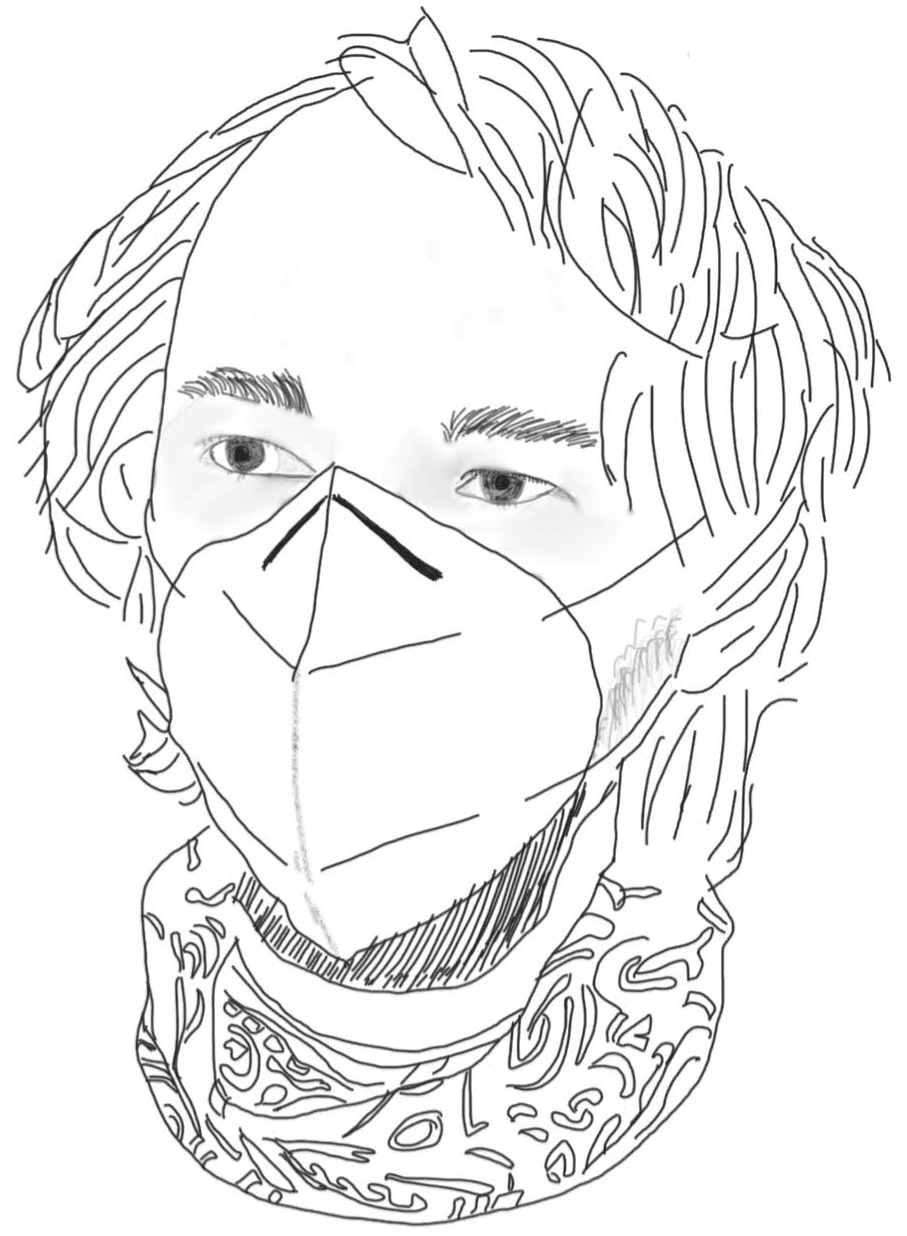
\includegraphics[height=2.5cm]{images/maskavatar-trimmed.jpg}
  \end{minipage}

  \vspace{5mm}
  \noindent
  
\includegraphics[height=1.8cm]{images/payments/qr-btc.pdf}\hspace{0.5cm}%
  
\includegraphics[height=1.8cm]{images/payments/qr-eth.pdf}\hspace{0.5cm}%
  \href{https://paypal.me/ralienpp}{
\includegraphics[height=1.8cm]{images/payments/qr-paypal.pdf}}%
  \hfill
  \href{https://creativecommons.org/licenses/by-sa/4.0/}{\includegraphics[height=0.4cm]{images/cc-by-sa-eps-converted-to.pdf}}
}

\end{document}
"
%
%  Positions differ from main.tex: stacked blocks are taller, so several
%  bottom-anchored text blocks are moved up to keep both languages on the
%  page. main.tex is unchanged.
% ============================================================
\documentclass[17pt]{extarticle}

% --- Language configuration (override before \input to change) ---
\ifdefined\booklang\else\def\booklang{ro}\fi
\ifdefined\booklangsecondary\else\def\booklangsecondary{en}\fi

\def\bookfont{Antykwa Torunska}
%\def\bookfont{OpenDyslexic}
%\def\bookfontpath{fonts/opendyslexic/}
\usepackage[pagenumbers]{picturebook}
\usepackage{multicol}
\usepackage{hyperref}

% Secondary-language styling (optional overrides):
%   \renewcommand{\dualsecstyle}{\small\itshape}
%   \renewcommand{\dualsep}{\par\smallskip}

\begin{document}

% ============================================================
%  COVER (p.1) — modern city   [single language: primary]
% ============================================================
\pagenumbersoff
\singlepage{images/cover.jpeg}{1}{1}{12.8}{%
		\begin{center}
			{\Huge\bfseries \tr{title}}\\[0.5cm]
			{\large \tr{subtitle}}
		\end{center}
}
\block{1}{18}{12.8}{%
	\begin{center}
		{\small \tr{series}}
	\end{center}
}

% ============================================================
%  2x single pp.2–3 — horse tram era
% ============================================================
\pagenumberson
\singlepage{images/modern-city.jpeg}{3.5}{1}{10}{%
	\begin{halo}[color=white, opacity=0.3]
		\dualtr{p01_modern_city}
	\end{halo}
}


\singlepage{images/horse-tram.jpeg}{1}{1}{12.8}{%
	\begin{halo}[color=white, opacity=0.3]
		\dualtr{p02_horse_tram}
	\end{halo}
}

% ============================================================
%  p.4 — growing cities, growing horse population
% ============================================================
\singlepage{images/riders-carriages.jpeg}{1.5}{1}{8}{%
	\begin{halo}[color=white, opacity=0.5]
		\dualtr{p03_growing_cities}
	\end{halo}
}
% moved up (18 -> 15.5) to fit the stacked second language
\block{1}{15.5}{8}{%
	\begin{halo}[color=white, opacity=0.5]
		\dualtr{p03a_more_horses}
	\end{halo}
}

% ============================================================
%  p.5 — New York 1890 statistics
% ============================================================
% moved up (10 -> 8) to fit the stacked subtitle + second language
\singlepage{images/horse-human-pseudotessellation.png}{1}{8}{12.8}{%
	\begin{halo}[color=white, opacity=0.75]
		\dualtr{p04_ny_stats}

		\bigskip
		\dualtr{p04_ny_subtitle}
	\end{halo}
}

% ============================================================
%  SPREAD pp.6–7 — daily horse waste / smell
% ============================================================
\fullspread{images/horse-output.jpeg}%
{1}{1}{12}{% left page
	\begin{halo}[color=white, opacity=0.3]
		\dualtr{p05_manure_stats}

		\bigskip
		\dualtr{p05_subtitle}
	\end{halo}
}%
{2}{1}{10}{% right page — centered question
	\begin{halo}[color=white, opacity=0.3]
		\begin{center}
			{\Large\bfseries \dualtr{p06_smell}}
		\end{center}
	\end{halo}
}

% ============================================================
%  p.8 — alarming situation, people adapting
% ============================================================
\singlepage{images/street-manure.jpeg}{1}{0.5}{12.8}{%
	\begin{halo}[color=white, opacity=0.3]
		\dualtr{p07_alarming}
	\end{halo}
}

% ============================================================
%  p.9 — saved by technology (old car)
% ============================================================
% moved up (18 -> 14.5) — bottom-anchored block grows downward when stacked
\singlepage{images/benz-motorwagen.jpeg}{1}{15}{12.8}{%
	\begin{halo}[color=white, opacity=0.4]
		\dualtr{p08_saved_by_tech}
	\end{halo}
}

% ============================================================
%  SPREAD pp.10–11 — history repeats / growing cars
% ============================================================
\singlepage{images/car-human-pseudotessellation.jpeg}{2}{8}{10}{%
	\begin{halo}[color=yellow, opacity=0.5]
	\begin{center}
		{\Large\bfseries \dualtr{p09_history_repeats}}
	\end{center}
	\end{halo}
}


\singlepage{images/gridlock.jpg}{1}{1}{12}{%
	\begin{halo}[color=white, opacity=0.3]
		\dualtr{p10_cars_growing}
	\end{halo}
}

% ============================================================
%  p.12 — cars produce invisible exhaust
% ============================================================
\singlepage{images/shrouded-in-exhaust-gas-clear.jpeg}{1}{0.8}{12.8}{%
	\begin{halo}[color=white, opacity=0.3]
		\dualtr{p11_exhaust}
	\end{halo}
}

% ============================================================
%  p.13 — can be smelled / detected
% ============================================================
\singlepage{images/shrouded-in-exhaust-gas.jpeg}{1}{0.8}{12.8}{%
	\begin{halo}[color=white, opacity=0.3]
		\dualtr{p12_detect}
	\end{halo}
}

% ============================================================
%  SPREAD pp.14–15 — health effects / piles haven't disappeared
% ============================================================
\fullspread{images/coughing.jpeg}%
{1}{1}{12.8}{% left page
	\begin{halo}[color=white, opacity=0.3]
		\dualtr{p13_health}
	\end{halo}
}%
{2}{1}{10}{% right page — dramatic
	\begin{halo}[color=white, opacity=0.3]
		\begin{center}
			{\Large\bfseries \dualtr{p14_piles_back}}
		\end{center}
	\end{halo}
}

% ============================================================
%  p.16 — what can you do?
% ============================================================
\singlepage{images/what-can-i-do.jpeg}{2}{1}{10}{%
	\begin{halo}[color=white, opacity=0.8]
		\begin{center}
			{\Large\bfseries \dualtr{p15_what_can_you_do}}
		\end{center}
	\end{halo}
}

% ============================================================
%  p.17 — walk, bike, public transport
% ============================================================
\singlepage{images/walk.jpeg}{1}{1}{12.8}{%
		\begin{center}
			\dualtr{p16_walk}
		\end{center}
}


\singlepage{images/cyclists.jpeg}{1}{1}{12.8}{%
		\begin{center}
			\dualtr{p16_bike}
		\end{center}
}

\singlepage{images/train-valley.jpg}{1}{2}{12.8}{%
		\dualtr{p16_public_transport}
}

\singlepage{images/remote-call.jpeg}{1}{1}{12.8}{%
		\begin{center}
			\dualtr{p16_stay}
		\end{center}
}

% ============================================================
%  p.18 — plant a tree
% ============================================================
% moved up (17 -> 15) to fit the stacked second language
\singlepage{images/plant-tree.jpeg}{1}{17}{12.8}{%
		\dualtr{p17_plant_tree}
}

% ============================================================
%  p.19 — use your vote
% ============================================================
\singlepage{images/vote.jpeg}{7}{1}{7}{%
		\dualtr{p18_vote}
}

% ============================================================
%  p.20 — contribute to tech progress
% ============================================================
% moved up (19 -> 16.5) to fit the stacked second language
\singlepage{images/science.jpeg}{1}{16.5}{12.8}{%
	\begin{halo}[color=white, opacity=0.8]
		\dualtr{p19_tech_progress}
	\end{halo}
}


% ============================================================
%  p.21,22 — think about the ecosystem
% ============================================================

\fullspread{images/planet.jpeg}%
{2}{1}{10}{% left page
	\begin{center}
		{\Large\bfseries \dualtr{p20_ecosystem}}
	\end{center}
}%
{2}{1}{10}{% 
	
}

% ============================================================
%  PROSE SECTION — parent guide   [single language: primary]
% ============================================================
\pagenumberson
\pagenumberstyle{center}
\startprose
\section*{\tr{parent_guide_title}}
{\small \tr{parent_guide_body}}

% ============================================================
%  GLOSSARY — vocabulary with IPA and translations
% ============================================================
\ifdefined\bookglossaryoff\else
  \newpage
  \section*{\tr{glossary_title}}

  \printglossary{translations/glossary.csv}{\booklang}{\booklangsecondary}
\fi

% ============================================================
%  BACK COVER
%  Pad to a full saddle-stitch signature (multiple of 4 pages) so
%  the back cover lands on the physical back-cover surface.
% ============================================================
\padbooklet
\backcover{%
  {\noindent\textbf{\tr{other_books_title}}\par\smallskip}
  \begin{bookgrid}
	\book{images/covers/cat-tree.png}{Poetry for kids}
    \book{images/covers/cover-high5.png}{What is software engineering?}
	\book{images/covers/tree-cover.jpeg}{Never give up}
  \end{bookgrid}

  \vfill

  {\noindent\textbf{\tr{about_author_title}}\par\smallskip}
  \noindent
  \begin{minipage}[t]{0.75\textwidth}
    \footnotesize
    \tr{about_author_body}
  \end{minipage}%
  \hfill
  \begin{minipage}[t]{0.2\textwidth}
    \raggedleft
    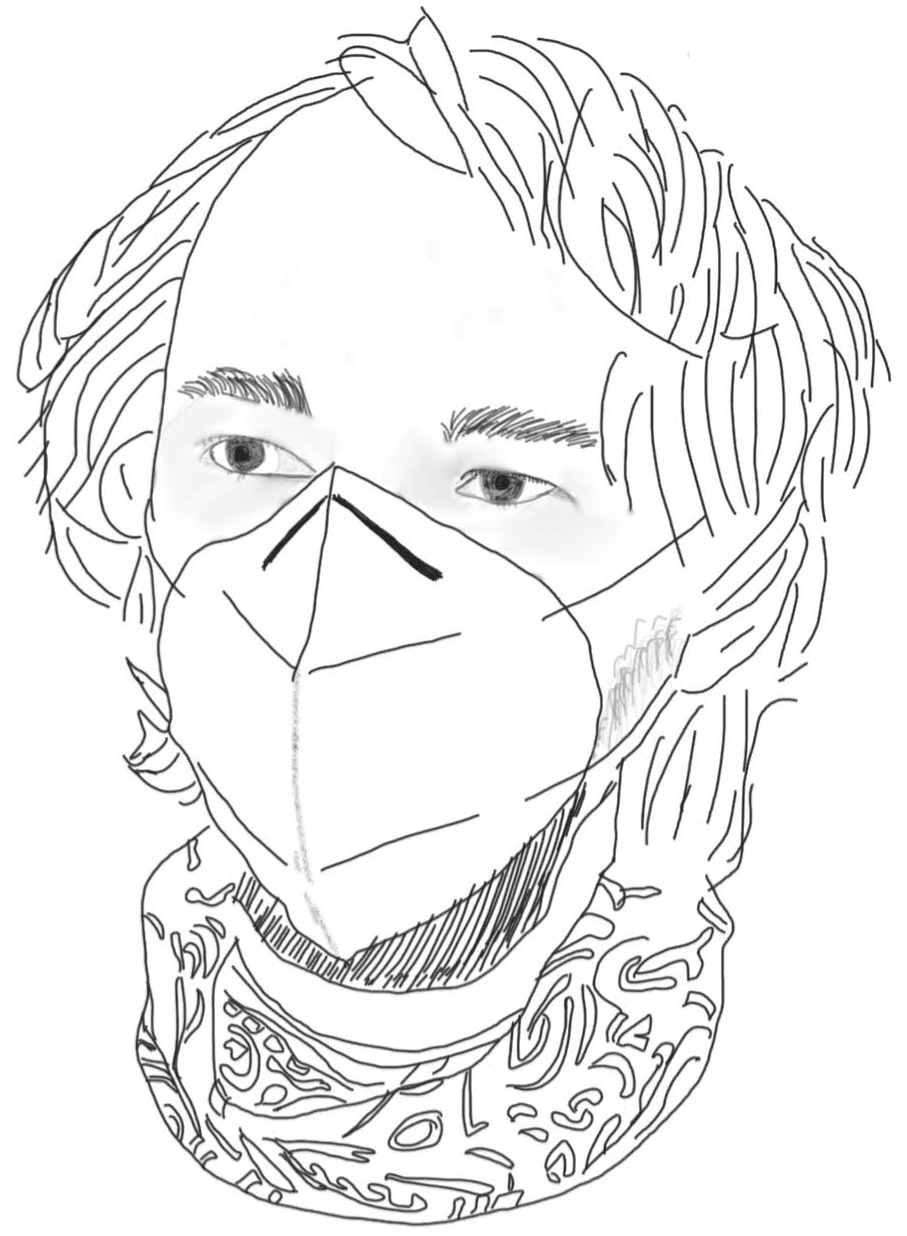
\includegraphics[height=2.5cm]{images/maskavatar-trimmed.jpg}
  \end{minipage}

  \vspace{5mm}
  \noindent
  
\includegraphics[height=1.8cm]{images/payments/qr-btc.pdf}\hspace{0.5cm}%
  
\includegraphics[height=1.8cm]{images/payments/qr-eth.pdf}\hspace{0.5cm}%
  \href{https://paypal.me/ralienpp}{
\includegraphics[height=1.8cm]{images/payments/qr-paypal.pdf}}%
  \hfill
  \href{https://creativecommons.org/licenses/by-sa/4.0/}{\includegraphics[height=0.4cm]{images/cc-by-sa-eps-converted-to.pdf}}
}

\end{document}
